% Phd Thesis

% Packages
\documentclass[a4paper]{book}
\usepackage{graphicx} % Required for inserting images
\usepackage{pdfpages} % Required for inserting PDFs
\usepackage[hidelinks]{hyperref} % Required for phantom sections
\usepackage[Sonny]{fncychap} % Required for chapter themes
\usepackage{longtable} % for tables
\usepackage{xurl} % For wrapping URLs
\usepackage{pdflscape}   % For rotating the page
\usepackage{array} % For better column formatting
\usepackage{booktabs} % For table formatting
\usepackage{fontspec} % Required to set fonts
\usepackage{setspace} % Required to set line spacing
\usepackage{fancyhdr} % Required for header and footer
\usepackage[backend=biber, style=vancouver]{biblatex} % for overleaf referencing
\AtEveryBibitem{%
  \ifentrytype{article}{%
    \clearfield{issn}%
    \clearfield{doi}%
    \clearfield{url}%
    \clearfield{urldate}%
    \clearfield{note}%
  }{}%
}
\addbibresource{refs/ch-1.bib} % Zotero ref library ch1
\addbibresource{refs/ch-6.bib} % Zotero ref library ch6
\addbibresource{refs/ch-9.bib} % Zotero ref library ch9
\addbibresource{refs/ch-ten.bib} % Zotero ref library ch10
\raggedbottom % make sure line spacing is the same on all pages, means text doesn't always end at bottom of page

% Ensure chapter titles are single spaced
\makeatletter
\let\old@makechapterhead\@makechapterhead
\renewcommand{\@makechapterhead}[1]{%
  {\singlespacing
   \old@makechapterhead{#1}}}
\makeatother

% Define reference syle for written chapters
\defbibheading{subbibliography}[\refname]{%
  \section{#1}%
}

% Document information
\title{Methods to Include Environmental Impacts in Health Technology Assessments}
\author{Jake Thomas Warton Williams}
\date{2025}

% Basic formatting---------------------------
\setmainfont{Times New Roman} % Font
\doublespacing % double line spacing
\pagestyle{plain}

%---------------------------------------------

\begin{document}

\frontmatter % Front matter
%\begin{singlespace}
    %\maketitle
    \begin{titlepage}
   \begin{center}

        \vspace*{2cm}
        
       \begin{Large}
       \textbf{Methods to include environmental impacts in health technology assessments}\par
       \end{Large}
            
       \vfill

       Jake Thomas Warton Williams BSc MPH

       \vfill
            
       A thesis submitted to fulfil the requirements of the degree of\\Doctor of Philosophy  
       
       \vfill
     
       %
\includegraphics[width=0.6\textwidth]{front-matter/university.jpeg}

       %\vfill
            
       School of Public Health\\
       Faculty of Medicine and Health\\
       University of Sydney

        \vfill

       2026
       
       \vspace*{2cm}

   \end{center}
\end{titlepage}
%\end{singlespace}
\chapter{Originality}
This is to certify that the content of this thesis is my own work. This thesis has not been submitted for any other degree or purpose. I certify that the intellectual content of this thesis is the product of my own work, and that all assistance received in preparing this thesis and all sources have been acknowledged.

\vspace{1cm}

% \includegraphics[height=2cm]{front-matter/williams_sig.png}

Jake T W Williams \hspace{2cm} 19 December 2025
\chapter{Abstract}
In the Australian health system, Government reimbursement decisions are often made on the basis of opportunity costs. The methods used to inform these decisions are health economic evaluation and health technology assessment. These consider the costs and consequences of alternative courses of action and have not traditionally considered environmental impacts. 

There is interest in Australia and elsewhere in understanding methods to include environmental impacts in health technology assessment in the pursuit of minimising the environmental and climate change impact of health technologies. 

The aim of this thesis was to evaluate methods to include environmental impacts in health economic evaluations and health technology assessments in the Australian reimbursement decision-making context. 

Chapter 1 introduces the research and frames the aims and objectives of the thesis.

Chapter 2 outlines the methods and structure of the thesis.

Chapter 3 shows environmental impacts can be estimated alongside costs in a cost analysis and demonstrates this using the same economic methods that identify, measure, and value resources.

Chapter 4 identifies at least four approaches and ten methods to include environmental impacts in health economic evaluations, many of which have not been demonstrated with empirical evidence. 

Chapter 5 estimates the health system costs and carbon emissions of diagnostic imaging by patients treated for stage III melanoma on different PET/CT surveillance schedules. 

Chapter 6 estimates the carbon footprint of full skin examination, total body photography, and the excision of a lesion suspicious for melanoma using process-based life cycle assessment methods.  

Chapter 7 demonstrated parallel and integrated methods to include carbon emissions in a cost-effectiveness analysis of 12-monthly PET/CT imaging for patients treated for stage III melanoma.

Chapter 8 describes items to include in a health economic analysis plan (HEAP) to describe the planned economic evaluation of a randomised controlled trial. 

Chapter 9 discusses methods to include environmental impacts in health technology assessment in the Australian policy context and proposes a simple decision matrix for the cost-minimisation analysis pathway.

Chapter 10 discusses the findings of the thesis.

The thesis found that economic evaluation frameworks are a useful way to estimate and present the environmental impact of health technologies. Further work is needed to understand how these can most usefully be implemented to inform HTA decisions in Australia and globally. 
\chapter{Acknowledgements}

It is a daunting task to acknowledge all the people who made this thesis possible. When I started my candidature almost four years ago, sitting at the same desk in the Edward Ford Building that I am sitting at now, I had no idea how important these people would be. I remember thinking at some point in my second year that I'd managed to avoid the stress of the stereotypical PhD candidate. I wasn't working weekends, I had used all my annual leave, and my caffeine addiction was about as bad as it had been before I started. But when that inevitably changed and the weight of this work fell heavily on my shoulders, this work was only possible because of the people who supported me.

First, to my supervisors. Professor Rachael Morton, for calmly guiding me through the final year of my candidature, and Dr Mbathio Dieng, for supporting me at the start of this journey when everything was new and uncertain. Professor Katy Bell, for opening the doors of academia and always making time for me. Dr Scott McAlister, for providing consistent technical expertise. It has been a pleasure working with you all and I offer you my deepest thanks.

To my colleagues and supervisors outside my PhD. The MEL-SELF team, Professor Paul Beggs, Professor Ying Zhang, and everyone at the Lancet Countdown Oceania and the Heat and Health Research Centre. Thank you for inspiring me and giving me opportunities to learn and grow.

Second, to my friends and family. You won’t find them listed as authors of any of the chapters presented in this thesis, but know that it does not exist without them. Because they loved me, fed me, made me laugh, watched movies with me, and were always proud of me. Even if they couldn't tell you with much certainty what this thesis is actually about. 

To my family. My parents Kathy and Richard, brother Dylan, and partner Luke. Thank you for raising me, for loving me, and for knowing exactly what to say and when to say it.

To my friends at work. Thank you for making this experience unforgettable. To Amber, Katie, and Phil, for being my first PhD friends and reminding me that work should be fun. To Amber (again), for never letting me call myself a fake health economist. To Joe, for teaching me to love R and Newtown Pork Roll. To Philomena, for being my colleague four times (and counting). To Ellie, for being on this journey with me since day one. You each made coming to the office a joy.

To my favourite people. Claudia, Connor, Jaimi, Dan, and Elysse, for growing up with me, loving me, and being with me in all the non-academic parts of this experience. 

This thesis will soon be a memory of the time I spent on it. Despite any venting I may have done, and the stress of these final few months, I have loved this experience and learnt so much from it. More than anything, I realise how much I do not know. I hope that never changes.
\chapter{Author attribution}

I, Jake T W Williams (JW), conducted this research during my candidature for a Doctor of Philosophy between 2021 and 2025 at the University of Sydney School of Public Health. I conducted this research under the guidance of my supervisors Professor Rachael L Morton (RM), Professor Katy J L Bell (KB), Dr Mbathio Dieng (MD), and Dr Scott McAlister (SM). Other contributors to this work were Professor Pascale Guitera (PG), Professor Linda K Martin (LM), Professor Madeleine Skellern (MS), and Associate Professor Rebecca Haddock (RH). The contribution of each person is provided in detail below. This detail is consistent with the contribution statements included with published chapters. No content produced by generative AI tools has been used in the preparation of this thesis.

Chapter 1 of this thesis was written by JW with critical review by RM.

Chapter 2 of this thesis was written by JW with critical review by RM.

Chapter 3 of this thesis was published as `Exploring the integration of environmental impacts in the cost analysis of the pilot-MEL-SELF trial of patient-led melanoma surveillance' in the journal \textit{Applied Health Economics and Health Policy}. Data analysis was conducted by JW under the supervision of MD. The chapter was written by JW with critical review by MD, RM, and KB.

Chapter 4 of this thesis was published as `Methods to include environmental impacts in health economic evaluations and health technology assessments: a scoping review' in the journal \textit{Value in Health}. The concept and design, analysis and interpretation of data, and critical review of the chapter was conducted by JW, KB, RM, and MD. Data was acquired by JW, RM, and MD. The manuscript was drafted by JW, KB, MD. Funding was acquired by JW, KB, and MD. Supervision was provided by KB, RM, MD.

Chapter 5 of this thesis was published as `Healthcare costs and carbon emissions of stage III melanoma surveillance imaging' in the journal \textit{Applied Health Economics and Health Policy}. The chapter was conceptualised, investigated, designed, resourced, and validated by JW, MD, KB, SM, and RM. Data curation, formal analysis, administration, software, visualisation, writing of the original draft was conducted by JW. Funding was acquired by JW, KB, and RM. Supervision was provided by MD, KB, SM, and RM. Critical review of the manuscript was provided by MD, KB, SM, and RM. 

Chapter 6 of this thesis is based on a manuscript titled `The carbon footprint of surgical and non-surgical skin cancer appointments' being reviewed by the journal \textit{Clinical and Experimental Dermatology}. The chapter was conceptualised by JW, KB, RM, and SM. Data curation, data analysis, validation, and visualisation was conducted by JW and SM. Funding acquisition, project administration, and software was conduced by JW. Supervision was provided by KB, RM, and SM. Investigation, methodology, resources, and critical review of the manuscript was provided by JW, KB, RM, PG, LM, and SM.

Chapter 7 of this thesis was published as `Methods to include environmental impacts in a cost-effectiveness analysis: a case study of surveillance imaging after treatment for stage III melanoma' in the journal \textit{Value in Health}. The chapter was conceptualised by JW, RM, KB, and SM. Data analysis was conducted by JW under the supervision of RM. The chapter was written by JW with critical review by RM, KB, and SM. 

Chapter 8 of this thesis was published as `Towards Environmentally Extended Health Economic Analysis Plans: A Case Study for the MEL-SELF Trial' in \textit{Applied Health Economics and Health Policy}. The chapter was conceptualised by JW, KB, SM, and RM. Supervision was provided by KB, SM, and RM. The chapter was written by JW with critical review by KB, SM, and RM.

Chapter 9 of this thesis is based on a manuscript titled `Methods to include environmental impacts in Australia health technology assessment' prepared for journal publication. The chapter was conceptualised by JW, KB, SM, RH, MS, and RM. Supervision was provided by KB, SM, and RM. The chapter was written by JW with critical review by KB, SM, RH, MS, and RM.

Chapter 10 of this thesis was written by JW with critical review by RM. 

\vspace{1cm}

%\includegraphics[height=2cm]{front-matter/williams_sig.png}

Jake T W Williams \hspace{2cm} 19 December 2025

\vspace{1cm}

As lead supervisor for the candidature upon which this thesis is based, I can confirm that the
authorship attribution statements above are correct.

%\includegraphics[height=2cm]{front-matter/morton_sig.jpg}

\vspace{1cm}

Rachael L Morton \hspace{2cm} 19 December 2025


\chapter{Outputs during candidature}
The following works were published or presented during the period of my candidature. The relationship of each work to this thesis is stated in square brackets. 

\section*{First-author journal articles}
\begin{itemize}
    \item \textbf{Williams JTW}, Bell KJL, Morton RL, Dieng M. Exploring the Integration of Environmental Impacts in the Cost Analysis of the Pilot MEL-SELF Trial of Patient-Led Melanoma Surveillance. Appl Health Econ Health Policy. 2023 Jan 1;21(1):23–30. [Included in thesis as Chapter \ref{ch-3}]
    \item \textbf{Williams JTW}, Bell KJL, Morton RL, Dieng M. Correction: Exploring the Integration of Environmental Impacts in the Cost Analysis of the Pilot MEL-SELF Trial of Patient-Led Melanoma Surveillance. Appl Health Econ Health Policy. 2024 Mar 1;22(2):271–2. [Provided in Appendix \ref{ap-a}]
    \item \textbf{Williams JTW}, Bell KJL, Morton RL, Dieng M. Methods to Include Environmental Impacts in Health Economic Evaluations and Health Technology Assessments: A Scoping Review. Value in Health. 2024 June 1;27(6):794–804. [Included in thesis as Chapter \ref{ch-4}]
    \item \textbf{Williams JTW}, Moraga Masson F, McGain F, Stancliffe R, Pilowsky JK, Nguyen N, et al. Interventions to reduce low-value care in intensive care settings: a scoping review of impacts on health, resource use, costs, and the environment. Intensive Care Med. 2024 Dec 1;50(12):2019–30. [Not included in thesis]
    \item Colagiuri P*, \textbf{Williams JTW*}, Beggs PJ, Zhang Y. The Fossil Fuel Non-Proliferation Treaty: what it is, its importance for health, and why Australia should endorse it. Medical Journal of Australia. 2025;222(6):297–9. (*co-first author) [Not included in thesis] 
    \item \textbf{Williams JTW}, Dieng M, Bell K, McAlister S, Morton RL. Healthcare Costs and Carbon Emissions of Stage III Melanoma Surveillance Imaging. Appl Health Econ Health Policy. 2025. [Included in thesis as Chapter \ref{ch-5}]
    \item \textbf{Williams JTW}, Colagiuri P, Beggs PJ, Zhang Y. Disparities in health and climate change research funding: the funders and the funded. The Journal of Climate Change and Health. Accepted, in press. [Not included in thesis]
    \item \textbf{Williams JTW}, Colagiuri P, Beggs PJ, van Daalen KR, Vyas A, Malik A, Zhang Y. The carbon footprint of air travel to UN climate conferences has increased 25-fold over three decades. Communications Sustainability. Accepted, in press. [Not included in thesis]
    \item \textbf{Williams JTW}, Bell KJL, McAlister S, Morton RL. Methods to include environmental impacts in a cost-effectiveness analysis: a case study of PET/CT surveillance imaging after surgical treatment for stage III melanoma. Value in Health. In press. [Included in thesis as Chapter \ref{ch-7}]
    \item \textbf{Williams JTW}, Bell KJL, McAlister S, Morton RL. Towards environmentally extended health economic analysis plans: a case study for the MEL-SELF trial. Applied Health Economics and Health Policy. In press. [Included in thesis as Chapter \ref{ch-8}]
\end{itemize}

In addition, the following first author journal articles were prepared during the period of my candidature and have not yet been published.

\begin{itemize}
    \item \textbf{Williams JTW}, Bell KJL, Morton RL, Guitera P, Martin LK, McAlister S. The carbon footprint of surgical and non-surgical skin cancer appointments. Under review with the Clinical and Experimental Dermatology. [Included in thesis as Chapter \ref{ch-6}]
    \item \textbf{Williams JTW}, Bell KJL, McAlister S, Skellern M, Haddock R, Morton RL. Methods to include environmental impacts in Australian health technology assessments. Being prepared for submission. [Included in thesis as Chapter \ref{ch-9}]
\end{itemize}

\section*{Policy documents}
\begin{itemize}
    \item \textbf{Williams J} and Haddock R. Consideration of environmental impacts in health technology assessment. Australian Healthcare and Hospitals Association Limited, Australia. 2025 Jun 5, Deeble issues brief 58. Available from: \url{https://ahha.asn.au/resource/consideration-of-environmental-impacts-in-health-technology-assessment/} [Included in thesis as Appendix \ref{ap-i}]
    \item Colagiuri P, \textbf{Williams JTW}, Beggs PJ, MacGregor C, Zhang Y. The Lancet Countdown on Health and Climate Change 2025 Climate and Health Policy Brief for Australia. Lancet Countdown on Health and Climate Change Oceania, Australia. Available from: \url{https://lancetcountdown.org/wp-content/uploads/2025/12/The-Lancet-Countdown-Policy-Brief-for-Australia-2025.pdf} [Not included in thesis]
\end{itemize}

\section*{Conference presentations}
\begin{itemize}
    \item Exploring the integration of environmental impacts in the cost analysis of the pilot MEL-SELF trial. ISPOR Student Symposium (Australian Chapter), 2022 (oral). [Related to Chapter \ref{ch-3}]
    \item Exploring the integration of environmental impacts in the cost analysis of the pilot MEL-SELF trial. Population Health Congress, 2022 (oral). [Related to Chapter \ref{ch-3}]
    \item Environmental impacts can be added to other costs in health economic evaluations. Healthy Environments and Lives Conference, 2022 (poster) [Related to Chapter \ref{ch-3}]
    \item Methods to include environmental impacts in health economic evaluations and health technology assessments: a scoping review. U21 Health Sciences Group Doctoral Student Forum, 2023 (oral). [Related to Chapter \ref{ch-4}]
    \item Methods to include environmental impacts in health economic evaluations and health technology assessments: a scoping review. Australian Health Economics Society Conference, 2023 (oral). [Related to Chapter \ref{ch-4}]
    \item The cost and climate change impact of stage III melanoma surveillance imaging. Australian Health Economics Society Conference, 2024 (poster). [Related to Chapter \ref{ch-5}] 
    \item The cost and climate change impact of stage III melanoma surveillance imaging. Health Services Research Conference, 2024 (oral). [Related to Chapter \ref{ch-5}]
    \item Methods to include carbon emissions in a cost-effectiveness analysis: a case study of stage III melanoma surveillance imaging. Preventing Overdiagnosis, 2025 (oral). An abstract for this presentation was published in \textit{BMJ EvidenceBased Medicine}; 2025 Sept 1; 30(Suppl 1):A45-6. [Related to Chapter \ref{ch-5} and \ref{ch-6}]
\end{itemize}

\section*{Protocols}
\begin{itemize}
    \item \textbf{Williams JTW}, Bell K, Morton R, Dieng M. Methods for including environmental impacts in health economic evaluations and health technology assessments: a scoping review. Open Science Framework. 2025. [Included in thesis as Appendix \ref{ap-c}]
    \item \textbf{Williams JTW}, Bell K, Morton RL, Guitera P, Martin L, and McAlister S. The climate change impact of surgical and non-surgical skin cancer appointments: a process-based life cycle assessment. Open Science Framework. 2025. [Included in thesis as Appendix \ref{ap-e}]

\end{itemize}

\section*{Non peer-reviewed publications}
\begin{itemize}
    \item Bell K, Colagiuri P, \textbf{Williams J}. Patient Initiated follow up as a low carbon alternative for cancer surveillance. The Health Advocate. Issue 73, November 2023. [Not included in thesis]
    \item \textbf{Williams JTW}, Bell KJL, Morton RL, Dieng M. Can health technology assessments contribute to environmentally sustainable healthcare? Health Economics Connect. Autumn 2024. [Not included in thesis]
\end{itemize}
\chapter{Financial support}
This research was supported by an Australian Government Research Training Program Fee Offset Scholarship, a University of Sydney Faculty of Medicine and Health Research Centres Stipend Scholarship, and a University of Sydney Faculty of Medicine and Health Completion Scholarship. Additional funds for research and travel were received from the Healthy Environments and Lives (HEAL) National Research Network, which receives funding from the National Health and Medical Research Council (NHMRC) Special Initiative in Human Health and Environmental Change (Grant No. 2008937), the Wiser Healthcare Research Collaboration, and the Australian Healthcare and Hospitals Association Deeble Institute for Health Policy Research.
\begin{singlespace}
    \setcounter{tocdepth}{1}
    \tableofcontents
\end{singlespace}

\mainmatter % Main matter
\chapter{Introduction}
\label{ch-1}
\begin{refsection}[refs/ch-1.bib]
This thesis examines methods to include environmental impacts in health technology assessment (HTA), and this chapter introduces the key concepts underpinning its content. First, it describes how decisions in the healthcare system are made, introducing HTA and health economic evaluation. Second, it outlines the relationship between healthcare decisions and the environment, introducing the health impacts of climate change and healthcare sustainability. Third, it summarises existing work to include environmental impacts in HTA. It concludes with the objectives of the thesis.

\section{Making decisions in the health system}
Decisions about the health system are made daily. Patients must decide when to seek care, clinicians must decide what care to recommend, and those responsible for the funding and delivery of the health system must decide what care is made available for use. Drummond et al. characterise these as decisions of resource allocation—“who should do what to whom, with what healthcare resources, and with what relation to other health services.”\cite{drummond_methods_2015} This thesis focuses on decisions about which services, tests, and treatments receive Federal Government reimbursement to make them affordable at the point of care.

The remainder of this thesis refers to health services, tests, and treatments as \textit{technologies}, being “an intervention developed to prevent, diagnose or treat medical conditions; promote health; provide rehabilitation; or organise health delivery".\cite{orourke_new_2020} The intervention can be a test, device, medicine, vaccine, procedure, program, or system.\cite{orourke_new_2020}

Government reimbursement decisions about health technologies are made based on the \textit{opportunity cost} of those decisions equal to the value of the forgone use of those same resources. Imagine a world where there is no scarcity and the various resources required to deliver healthcare are unlimited. In this world decisions might only concern whether a technology is safe and expected to have health benefits. There would be no concern of resource depletion, as resources could be spent without consideration of their alternative use. However, this is not the world we live in, and the money, people, time, and energy required to deliver healthcare are finite and scarce. Therefore, when decisions are made to spend resources, they are done so at the expense of all other alternative use of those resources—their opportunity cost.

In many countries, including Australia, government healthcare reimbursement decisions are made based on opportunity costs. The methods used to inform decisions about opportunity costs are health economic evaluation and health technology assessment.

\subsection{Health economic evaluation}
\textit{Health economic evaluation} is “the comparative analysis of alternative courses of action in terms of both their costs and consequences”.\cite{drummond_methods_2015} It is principally concerned with evaluating the consequences of providing a healthcare technology relative to the costs required to do so and comparing this with alternative technologies. Figure \ref{fig:ch-1-fig-1}, adapted from Drummond et al., illustrates how comparative health economic evaluations are structured.\cite{drummond_methods_2015}

\begin{figure}
    \centering
    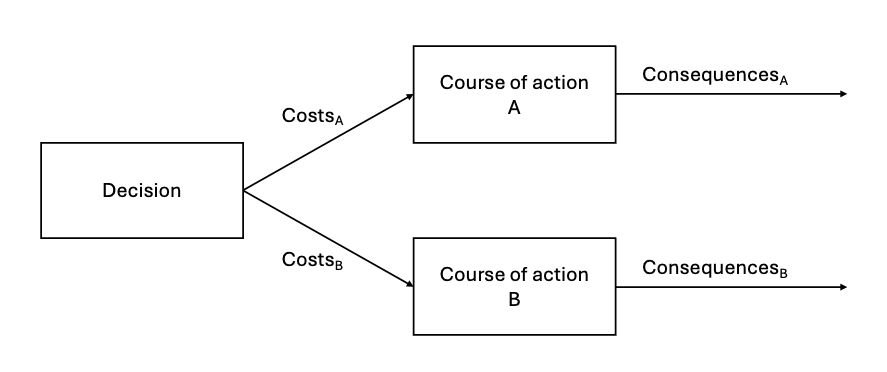
\includegraphics[width=1\linewidth]{core-chapters/figs/ch-1-fig-1.png}
    \caption{Illustration of the structure of health economic evaluations.}
    \label{fig:ch-1-fig-1}
\end{figure}

Study types for health economic evaluations vary based on the type of question they aim to inform, and the way health outcomes are measured. Several types are used in decision-making. These include \textit{cost-utility analysis} (CUA), \textit{cost-effectiveness analysis} (CEA), and \textit{cost-benefit analysis} (CBA). These three methods differ based the how health outcomes are valued, which can be in utility-weighted survival units (for CUA), health units (for CEA), or monetary units (for CBA). Other common types of analysis include \textit{cost-minimisation analysis} (CMA), where consequences are assumed to be equivalent and only costs are considered, and \textit{cost analysis}, a partial evaluation methods that compares costs only.

Debate persists about whether health economic evaluation should be \textit{welfarist} or \textit{extra-welfarist} in its approach.\cite{brouwer_welfarism_2008} Welfarist evaluations are concerned with maximising welfare and value all consequences with equivalent wellbeing equally. These evaluations consider all aspects of society and often take a \textit{societal perspective} in their analysis, including costs and consequences directly related to the individual, the health system, and non-health sectors. Extra-welfarist evaluations are concerned with maximising health outcomes and are typically undertaken from the \textit{health system perspective}, including only the consequences related to an individual’s health and the costs to the health system.

Regardless of the economic method, theoretical framework, or perspective chosen, health economic evaluations evaluate interventions in terms of their value-for-money and answer questions about the costs and consequences of competing alternatives. Historically, they have not included environmental impacts.

\subsection{Health technology assessment}
\textit{Health technology assessment} (HTA) is a process related to health economic evaluation that evaluates technologies in a specific decision context. It is used in many high-income countries with universal healthcare systems to inform decisions about government reimbursement. The International Network of Agencies for Health Technology Assessment (INAHTA) and Health Technology Assessment International (HTAi) define HTA as:
\begin{quote}
    ``a multidisciplinary process that uses explicit methods to determine the value of a health technology at different points in its life cycle. The purpose is to inform decision-making in order to promote an equitable, efficient, and high-quality health system."\cite{orourke_new_2020}
\end{quote}

HTA is used to inform decisions about which technologies are made available under one of the Australia’s universal access schemes: the Pharmaceutical Benefits Scheme (PBS), Medicare Benefits Schedule (MBS), National Immunisation Program (NIM), National Blood Agreement, or Prescribed List (PL), previously known as the prostheses list. HTA for this purpose is undertaken by the Pharmaceutical Benefits Advisory Committee (PBAC),\cite{australian_government_department_of_health_disability_and_ageing_guidelines_2016} Medical Services Advisory Committee (MSAC),\cite{australian_government_department_of_health_disability_and_ageing_guidelines_2021} and the Medical Devices and Human Tissue Advisory Committee (MDHTAC), who evaluate proposals submitted to them from applicants, such as pharmaceutical companies or device manufacturers. These committees advise the Minister for Health on whether, and under what circumstances, a technology should be recommended for reimbursement.\cite{australian_government_department_of_health_disability_and_ageing_guidelines_2016, australian_government_department_of_health_disability_and_ageing_guidelines_2021} The advice is primarily based on the comparative safety, effectiveness, cost-effectiveness (i.e., opportunity cost), and total cost of the technology, a focus that is common in HTA conducted for government reimbursement globally.\cite{world_health_organization_2015_2015}

Information about cost-effectiveness is obtained from within-trial and modelled economic evaluations of the health technology and its comparator. As with economic evaluation, environmental impacts have not traditionally been considered in HTA. However, there is interest in Australia and globally in understanding if this can be done.\cite{australian_government_department_of_health_and_aged_care_health_2024}

\section{Healthcare and climate change}
Health and climate change are connected in two ways. First, climate change has severe impacts on human health, and these are expected to worsen as the impacts of climate change continue. Second, health systems have large environmental impacts and are significant contributors to the greenhouse gas emissions causing climate change.

\subsection{Health impacts of climate change}
\textit{Climate change} is the ongoing increase in the Earth’s average temperature and its related impacts on weather and climate. The current period of climate change is being caused by human activity, primarily from \textit{greenhouse gas} (GHG) \textit{emissions}, such as carbon dioxide ($CO_{2}$), since the Industrial Revolution. The Sixth Report of the Intergovernmental Panel on Climate Change, released in 2023, found that global GHG emissions were the highest on record and that in the last decade average temperatures were 1.1 °C above pre-industrial levels.\cite{lee_climate_2023}

This increase in temperature is having devastating impacts on human health. The 2024 report of the Lancet-Countdown on health and climate change found record-breaking impacts to health and wellbeing.\cite{romanello_2024_2024} This includes direct impacts from heat, extreme weather events, infectious diseases, and food insecurity, and broader indirect economic and societal impacts.\cite{romanello_2024_2024}

Preventing the worst health impacts of climate change requires rapid reductions in GHG emissions to prevent further temperature increases. This is the ambition of the Paris Agreement, in which parties to the United National Framework Convention on Climate Change agreed to limit warming to 1.5 °C or well below 2 °C by achieving net-zero GHG emissions by 2050.

\subsection{Healthcare sustainability}
\textit{Healthcare sustainability} is variably defined and is generally used to describe efforts to reduce the environmental and climate change impact of the health system. It is focused on the demand and supply of healthcare technologies, mitigation and adaptation strategies, and decisions made at individual and system levels.\cite{mortimer_sustainable_2010, macneill_planetary_2021} This thesis is only concerned with matters of \textit{environmental sustainability} and how these relate to health technology assessment and health economic evaluation. We do not consider other types of sustainability that might also be covered by the label of ``healthcare sustainability".

The health sector has large environmental impacts. It accounts for about 5\% of national GHG emissions and in most countries is only exceeded by sectors related to energy, construction, and transport.\cite{pichler_international_2019, lenzen_environmental_2020} This is especially true for high-income countries with large health systems. In Australia, healthcare is responsible for 5\% to 7\% of total emissions.\cite{malik_carbon_2018, de_sain_estimates_2024} Most of this comes from the indirect impact of purchased goods and services required to deliver care, with only 27\% being attributable to direct emissions or energy use.\cite{de_sain_estimates_2024}

In a paper outlining the Campaign for Greener Healthcare in the United Kingdom, Mortimer identified four principles of sustainable clinical practice, as (1) disease prevention and health promotion, (2) patient education and empowerment, (3) lean service delivery, and (4) preferential use of treatment options and medical technologies with lower environmental impacts.\cite{mortimer_sustainable_2010} A recent framework by MacNeil, McGain \& Sherman describes a sustainable health system as one that reduces the demand of health services, matches supply of health services to demand, and reduces emissions from supply of health services.\cite{macneill_planetary_2021} Both of these approaches to sustainable healthcare emphasise decisions about the type of health technologies provided—decisions that can be informed by HTA. 

\section{Healthcare sustainability and health technology assessment}
Mortimer was one of the first to suggest healthcare decisions ought to consider environmental impacts, arguing in 2010 that the “inclusion of sustainability measures in the evaluation of medical technologies will allow service planners, clinicians and patients to choose clinically effective treatments with the best environmental profile and will encourage their further development.”\cite{mortimer_sustainable_2010} Mortimer did not suggest how this could be done, and it was several years before these ideas were developed further.

Between 2016 and 2020, health economists made substantial contributions to the question of whether environmental impacts can be used to inform health technology assessment, justifying several approaches and proposing methods for how it could be achieved. Marsh et al. were the first to argue that including environmental impacts in HTA is feasible from an economic perspective, outlining several methods that could be used to do so.\cite{marsh_expanding_2016} In a separate study, Marsh et al. demonstrated a simple method to include GHG emissions impacts in a modelled CEA, reporting total and incremental GHG emissions.\cite{marsh_incorporating_2016} This was the first empirical study demonstrating a method to include GHG emissions in a health economic evaluation. Later, de Preux and Rizmie demonstrated a similar method into include GHG emissions, but went a step further, valuing them in monetary units and including them as a cost in the incremental cost effectiveness ratio.\cite{de_preux_beyond_2018} In 2020, Hensher expanded on the work by Marsh et al. by also demonstrating the feasibility of valuing GHG emissions in monetary units.\cite{hensher_incorporating_2020}

In recent years there has been a considerable increase in the number of studies addressing the inclusion of environmental impacts in HTA and economic evaluation,\cite{polisena_environmental_2018, pinho-gomes_incorporating_2022, guirado-fuentes_main_2023, desterbecq_inclusion_2023, antonazzo_health_2025} and a detailed review of this literature is provided in Chapter \ref{ch-4} of this thesis. Much of this work is not specific to the Australian healthcare reimbursement decision-making context. 

\subsection{Australian policy context}
In Australia, HTA conducted to inform public reimbursement decisions are submitted by applicants for evaluation to the Medical Services Advisory Committee (MSAC) for medical interventions, the Pharmaceutical Benefits Advisory Committee (PBAC) for pharmaceuticals, and the Medical Devices and Human Tissue Advisory Committee (MDHTAC) for medical devices.

While these HTA focus on clinical and economic concerns, MSAC are currently able to consider other factors, including any relevant \textit{environmental aspects} of the technology.\cite{australian_government_department_of_health_disability_and_ageing_guidelines_2021} Guidelines for submissions to MSAC state, “if there are particular concerns regarding the environmental impact of the proposed health technology, or a key benefit in the way the proposed technology reduces the environmental impact compared with the comparator, these can be outlined”.\cite{australian_government_department_of_health_disability_and_ageing_guidelines_2021} It is therefore possible for MSAC to consider environmental impacts, however there is no evidence that this is being done, and MSAC has no further guidance on the topic. Guidelines for HTAs reviewed by PBAC and MDHTAC are silent on this matter and do not consider environmental aspects in their deliberations.\cite{australian_government_department_of_health_disability_and_ageing_guidelines_2016}

The Health and Climate Strategy, published in 2023, commits the Australian Government to review options to report and consider environmental impacts of health technologies in collaboration and alignment with international counterparts,\cite{australian_government_department_of_health_disability_and_ageing_national_2023} and this commitment was prioritised for implementation in 2024.\cite{australian_government_department_of_health_disability_and_ageing_national_2024} The Health Technology Assessment Policy and Methods Review, published in 2024, recommends the Australian Government investigate reporting environmental impacts during the assessment of cost-effectiveness and the potential to use this information in approval and reimbursement decisions.\cite{australian_government_department_of_health_and_aged_care_health_2024}

Despite these policies, there has been very little work to understand methods to include environmental impacts in HTA for the Australian context. 

\section{Case studies}
Two case studies for assessing environmental impacts were relied on throughout this thesis, both of which relate to the management of patients treated for melanoma of the skin. Australia has the highest incidence of melanoma in the world and this is a significant and growing health burden. After treatment, patients have a high risk of developing new primary melanomas and/or recurrence from their initial melanoma. Recommendations for the management of patients after treatment vary but include routine monitoring of the skin (to detect in-transit metastases or lymph node recurrence and new primary melanomas) and routine diagnostic imaging (to detect nodal or distant recurrence). 

The first case study involves the routine follow up of patients previously diagnosed with American Joint Committee on Cancer (AJCC) stage 0-II melanoma. The MELanoma SELF surveillance (MEL-SELF) randomised controlled trial (RCT) aimed to determine whether patient-led surveillance (smartphone supported skin self-examination, fast-tracked unscheduled visits as needed, usual care) compared with clinician-led surveillance (usual care), increases the proportion of participants diagnosed with a subsequent new primary melanoma at a fast-tracked unscheduled clinic visit.\cite{ackermann_can_2021} A pilot MEL-SELF RCT was previously completed.\cite{ackermann_assessing_2022} 

The second case study involves the routine follow up of patients previously diagnosed with AJCC stage III melanoma. After initial surgical treatment, patients undergo frequent diagnostic imaging tests, including positron emission tomography with computed tomography (PET/CT), to detect recurrent disease. A cohort of patients treated for stage III melanoma at the Melanoma Institute Australia between 2000 and 2014 was investigated.

\section{Objective}
The overall aim of this thesis is to evaluate methods to include environmental impacts in health economic evaluations and health technology assessments in the Australian reimbursement decision-making context.

The primary aims of the substantive parts of this thesis are to:
\begin{itemize}
    \item Describe potential methods to include environmental impacts in health economic evaluations and health technology assessments
    \item Demonstrate and evaluate methods to include environmental impacts in health economic evaluations
    \item Evaluate methods to include environmental impacts in Australian health technology assessment
\end{itemize}

\printbibliography[heading=subbibliography]
\end{refsection}
\chapter{Methods}
\label{ch-2}

This thesis contains ten chapters. The first two chapters introduce the research topic and outline the methods used. The middle seven chapters form the substantive part of the thesis and generate new knowledge. The final chapter discusses the findings of the research and concludes the thesis.

Chapter \ref{ch-3} aimed to describe and demonstrate an approach to include environmental impacts in a cost analysis. It used standard economic methods to understand the feasibility of doing so applied to the pilot MEL-SELF RCT. 

Chapter \ref{ch-4} aimed to review methods to include environmental impacts in health economic evaluations and health technology assessments. It used methods to conduct a scoping review recommended by JBI (formerly an acronym for the Joanna Briggs Institute).

Chapter \ref{ch-5} aimed to estimate the health system costs and associated carbon emissions of diagnostic imaging tests used by patients undergoing different surveillance schedules for Stage III melanoma follow up. It used epidemiological and economic methods to estimate the costs and carbon emissions of a defined patient cohort. The results of this chapter were used in the cost-effectiveness analysis reported in Chapter \ref{ch-7}.

Chapter \ref{ch-6} aimed to estimate the carbon emissions of appointments at a skin cancer clinic related to the identification and excision of lesions suspicious for melanoma and other skin cancer. It used process-based life cycle assessment methods to estimate carbon emissions of each type of appointment. The results of this chapter were used in the cost-effectiveness analysis reported in Chapter \ref{ch-7}.

Chapter \ref{ch-7} aimed to demonstrate methods to include carbon emissions in a cost-effectiveness analysis. It used standard economic methods for the base case analysis. Methods identified in Chapter \ref{ch-4} were used to include environmental impacts, and these were evaluated. 

Chapter \ref{ch-8} aimed to describe items to include in a health economic analysis plan (HEAP) to prespecify methods to include environmental impacts. The HEAP for the cost consequence analysis of the MEL-SELF trial was used as a case study. 

Chapter \ref{ch-9} aimed to outline the current Australian policy context for including environmental impacts in HTA, evaluate potential methods to include environmental impacts for public reimbursement, and detail a potential method for the cost-minimisation pathway. 

Chapter \ref{ch-10} summarises key findings, explores their implications for researchers and policy makers, and concludes the thesis.
\chapter{Exploring the integration of environmental impacts in the cost analysis of the pilot MEL-SELF trial of patient-led melanoma surveillance}
\label{ch-3}

The aim of this chapter was to describe and demonstrate an approach to include environmental impacts in a cost analysis. It was published in \textit{Applied Health Economics and Health Policy}. A correction to the original text was published in the same journal, details of which are provided in Appendix \ref{ap-a}.

\paragraph*{Publication details}
\textit{Williams JTW}, Bell KJL, Morton RL, Dieng M. Exploring the Integration of Environmental Impacts in the Cost Analysis of the Pilot MEL-SELF Trial of Patient-Led Melanoma Surveillance. Appl Health Econ Health Policy. 2023 Jan 1;21(1):23–30. 

% PDF of published paper
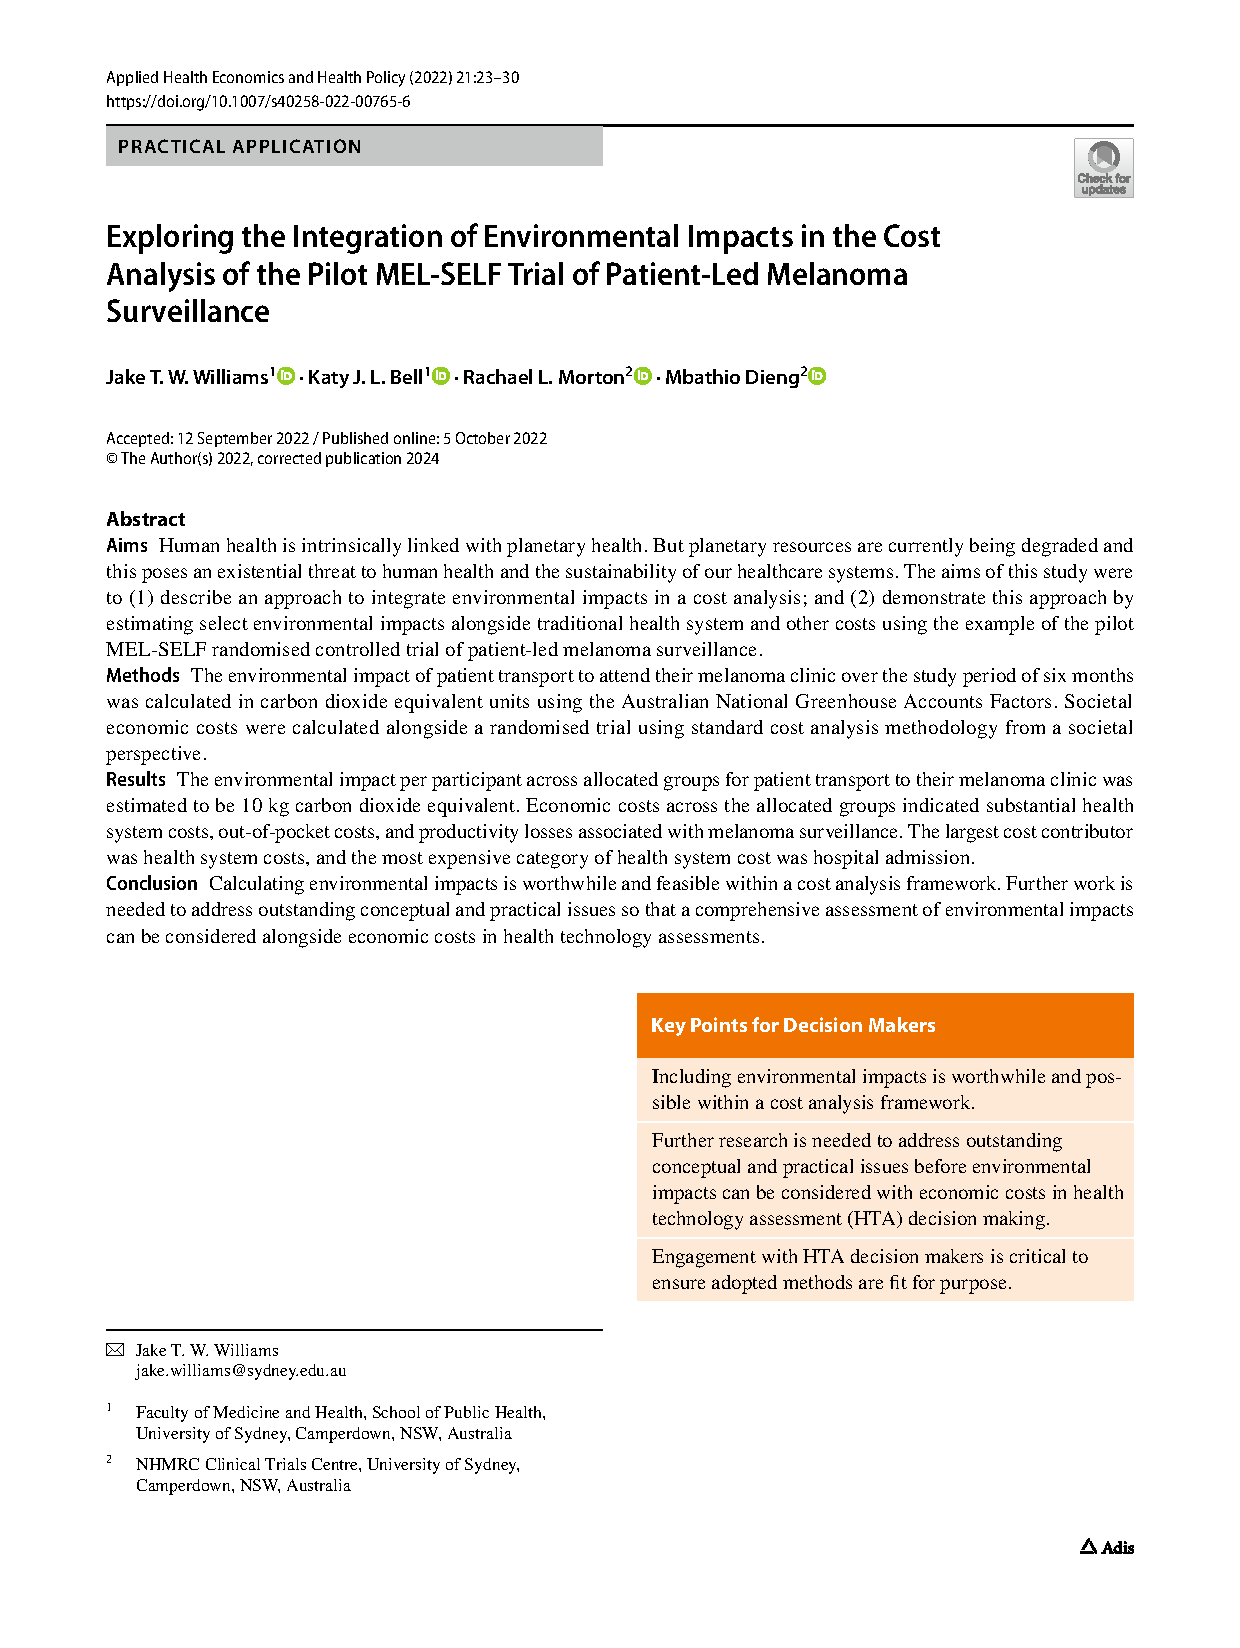
\includepdf[
  pages=1,
  pagecommand={
    \thispagestyle{empty}
    \addcontentsline{toc}{section}{\numberline{3.1}Abstract}
    \addcontentsline{toc}{section}{\numberline{3.2}Key points for decision makers}
  }
]{pdfs/ch-3.pdf}

\includepdf[
  pages=2,
  pagecommand={
    \thispagestyle{empty}
    \addcontentsline{toc}{section}{\numberline{3.3}Introduction}
    \addcontentsline{toc}{section}{\numberline{3.4}Methods}
  }
]{pdfs/ch-3.pdf}

\includepdf[
  pages=3,
]{pdfs/ch-3.pdf}

\includepdf[
  pages=4,
  pagecommand={
    \thispagestyle{empty}
    \addcontentsline{toc}{section}{\numberline{3.5}Results}
  }
]{pdfs/ch-3.pdf}

\includepdf[
  pages=5,
  pagecommand={
    \thispagestyle{empty}
    \addcontentsline{toc}{section}{\numberline{3.6}Discussion}
  }
]{pdfs/ch-3.pdf}

\includepdf[
  pages=6,
]{pdfs/ch-3.pdf}

\includepdf[
  pages=7,
  pagecommand={
    \thispagestyle{empty}
    \addcontentsline{toc}{section}{\numberline{3.7}References}
  }
]{pdfs/ch-3.pdf}

\includepdf[
  pages=8,
]{pdfs/ch-3.pdf}
\chapter{Methods to include environmental impacts in health economic evaluations and health technology assessments: a scoping review}
\label{ch-4}

The aim of this chapter was to summarise existing evidence about methods to include environmental impacts in health economic evaluations and health technology assessments. It was published in \textit{Value in Health}. Supplementary materials are provided in Appendix \ref{ap-b}. A protocol was published on the \textit{Open Science Framework} and is provided in Appendix \ref{ap-c}.

\paragraph*{Publication details}
\textit{Williams JTW}, Bell KJL, Morton RL, Dieng M. Methods to Include Environmental Impacts in Health Economic Evaluations and Health Technology Assessments: A Scoping Review. Value in Health. 2024 June 1;27(6):794–804. 


% PDF of published paper
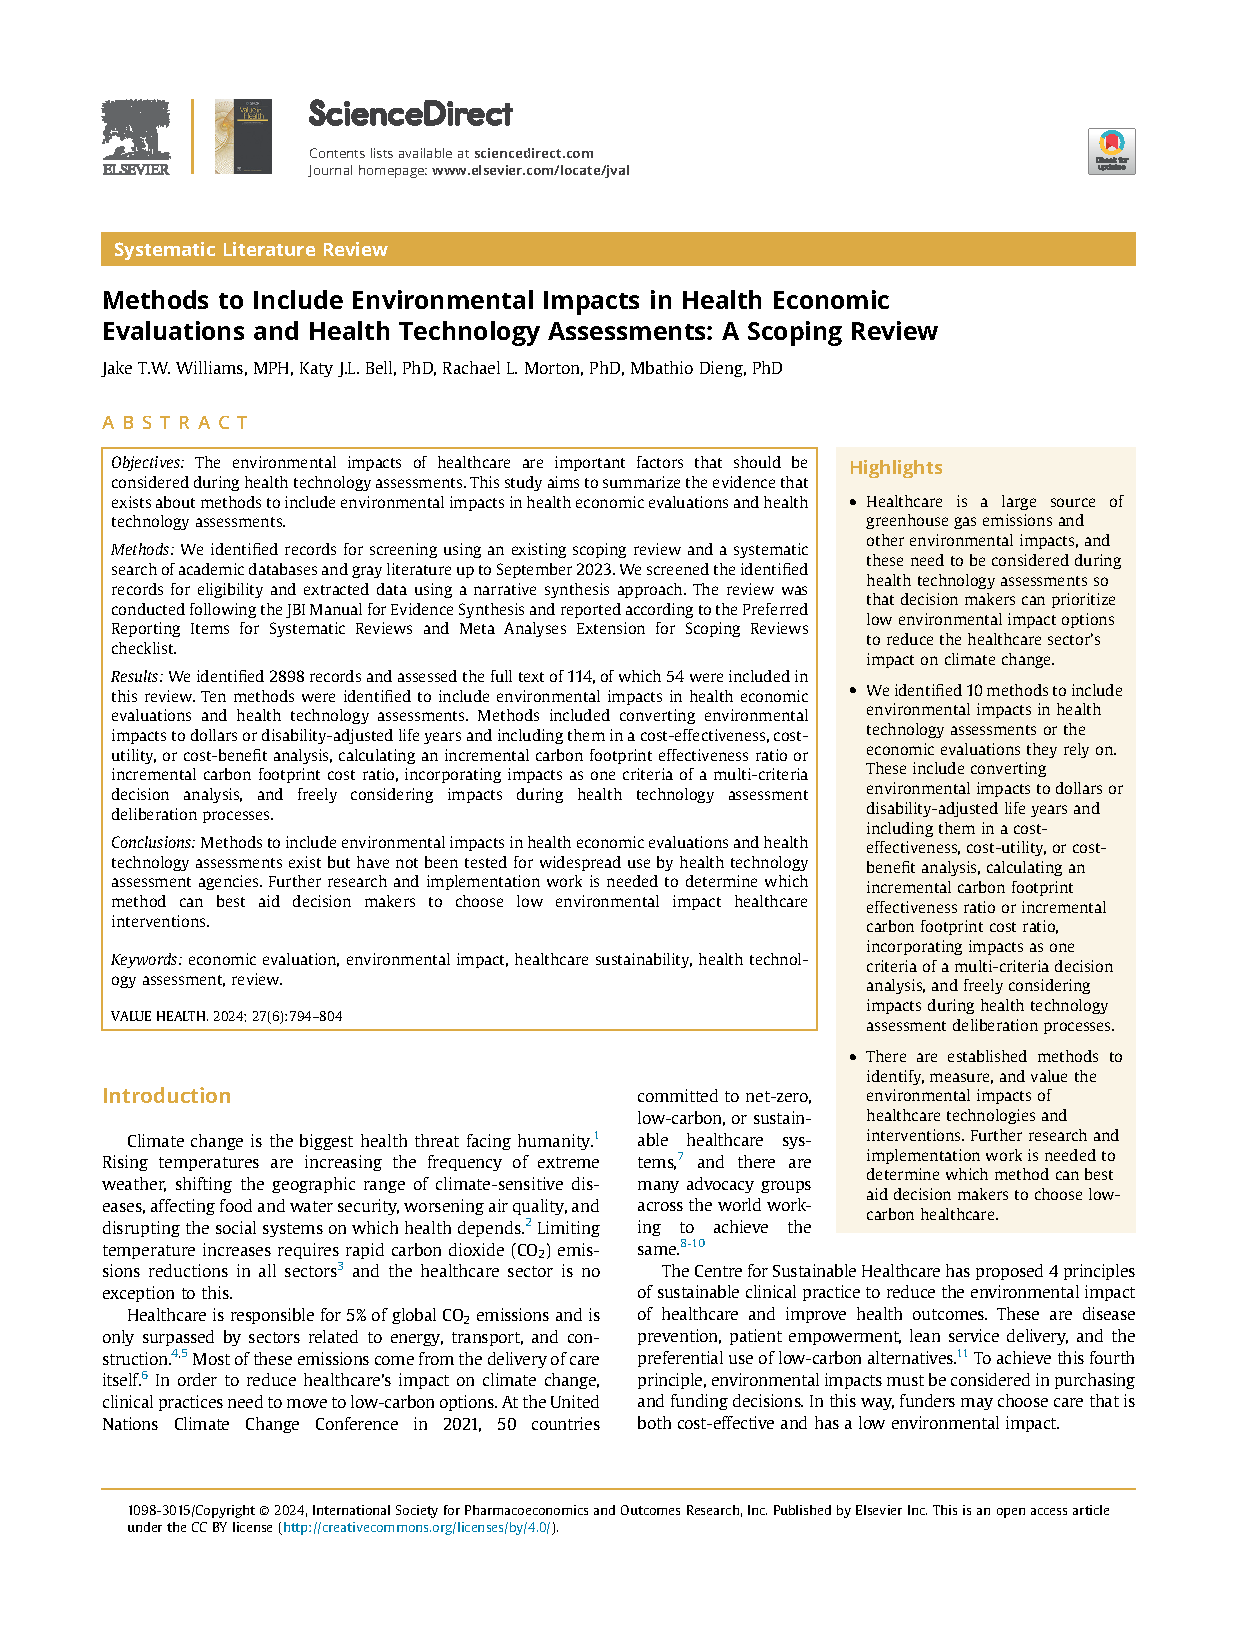
\includepdf[
  pages=1,
  pagecommand={
    \thispagestyle{empty}
    \addcontentsline{toc}{section}{\numberline{4.1}Abstract}
    \addcontentsline{toc}{section}{\numberline{4.2}Highlights}
    \addcontentsline{toc}{section}{\numberline{4.3}Introduction}
  }
]{pdfs/ch-4.pdf}

\includepdf[
  pages=2,
  pagecommand={
    \thispagestyle{empty}
    \addcontentsline{toc}{section}{\numberline{4.4}Methods}
  }
]{pdfs/ch-4.pdf}

\includepdf[
  pages=3,
  pagecommand={
    \thispagestyle{empty}
    \addcontentsline{toc}{section}{\numberline{4.5}Results}
  }
]{pdfs/ch-4.pdf}

\includepdf[
  pages=4,
]{pdfs/ch-4.pdf}

\includepdf[
  pages=5,
]{pdfs/ch-4.pdf}

\includepdf[
  pages=6,
]{pdfs/ch-4.pdf}

\includepdf[
  pages=7,
  pagecommand={
    \thispagestyle{empty}
    \addcontentsline{toc}{section}{\numberline{4.6}Discussion}
  }
]{pdfs/ch-4.pdf}

\includepdf[
  pages=8,
]{pdfs/ch-4.pdf}

\includepdf[
  pages=9,
  pagecommand={
    \thispagestyle{empty}
    \addcontentsline{toc}{section}{\numberline{4.7}References}
  }
]{pdfs/ch-4.pdf}

\includepdf[
  pages=10,
]{pdfs/ch-4.pdf}


\includepdf[
  pages=11,
]{pdfs/ch-4.pdf}

\chapter{Healthcare costs and carbon emissions of stage III melanoma surveillance imaging}
\label{ch-5}

The aim of this chapter was to estimate the health system costs and associated carbon emissions of diagnostic imaging tests used by patients undergoing different surveillance schedules for stage III melanoma follow up. It was published in \textit{Applied Health Economics and Health Policy}. Supplementary materials are provided in Appendix \ref{ap-d}.

\paragraph*{Publication details}
\textit{Williams JTW}, Dieng M, Bell K, McAlister S, Morton RL. Healthcare Costs and Carbon Emissions of Stage III Melanoma Surveillance Imaging. Appl Health Econ Health Policy.


% PDF of published paper
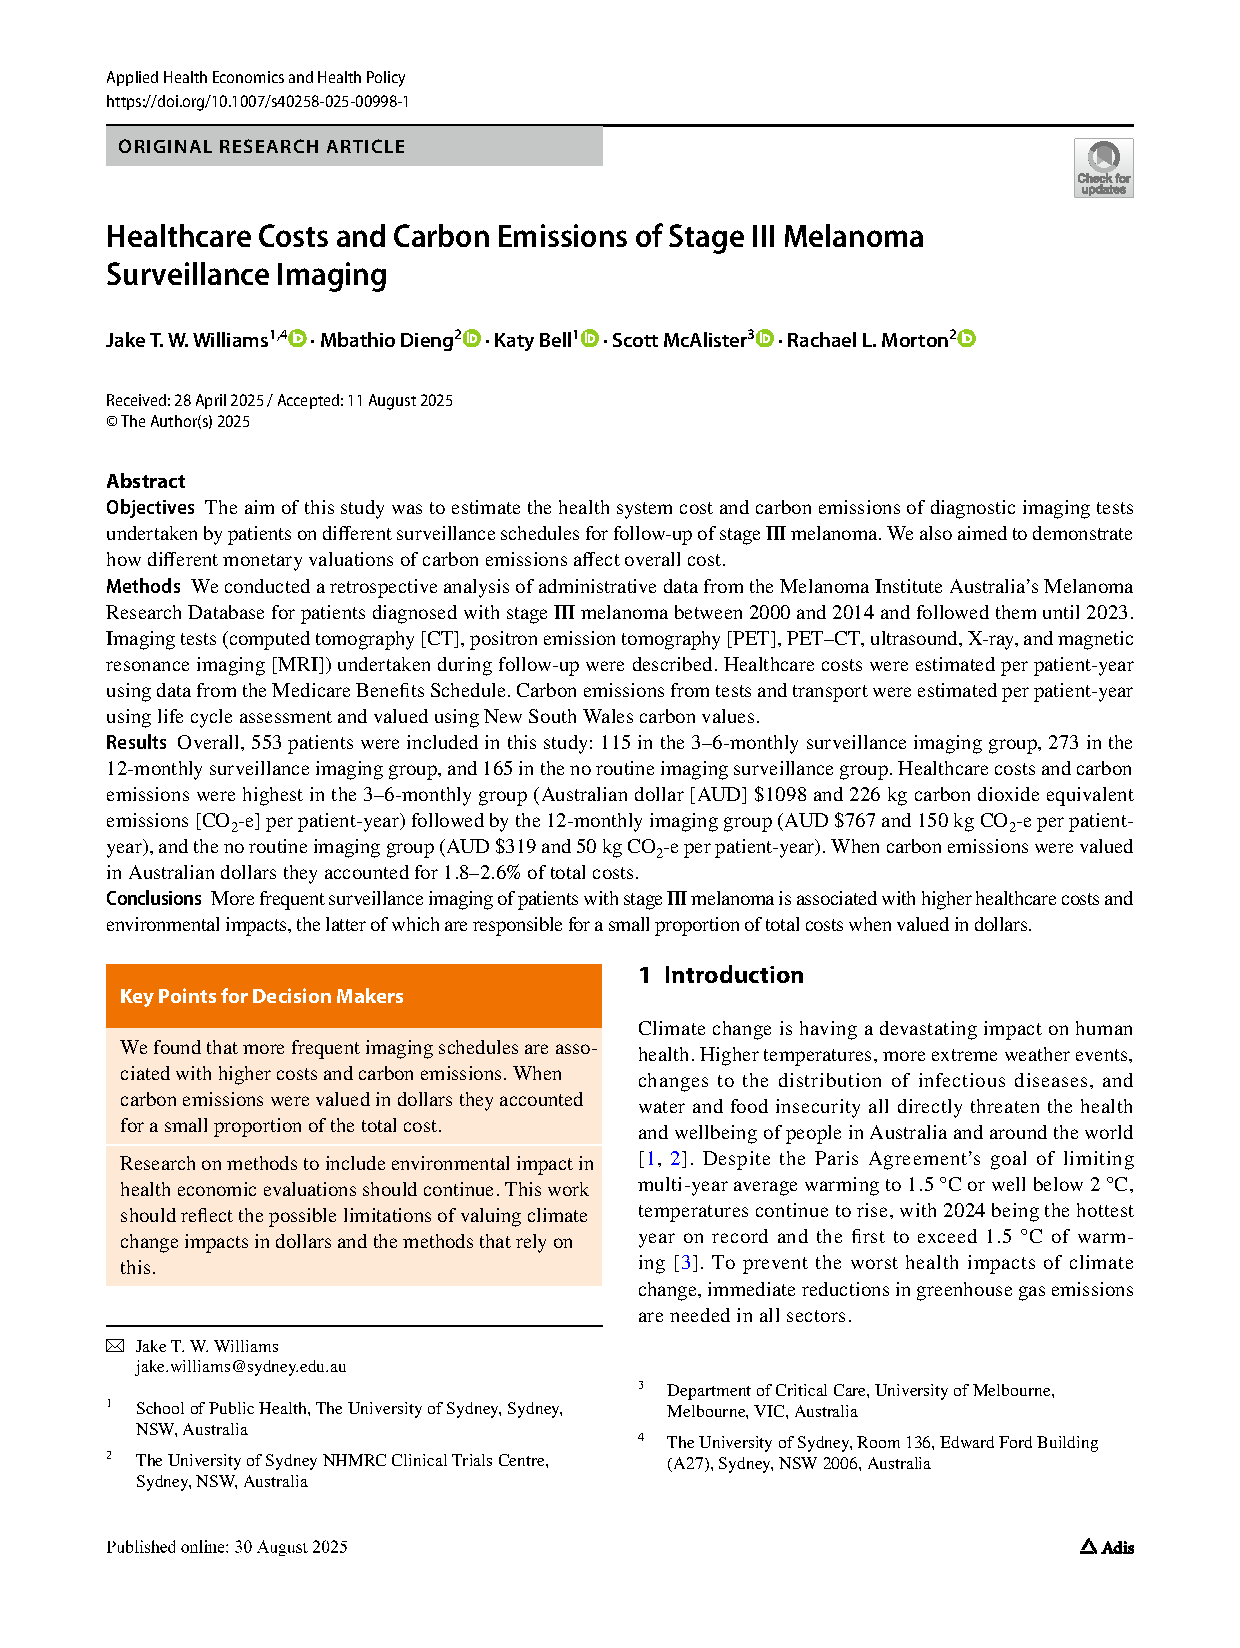
\includepdf[
  pages=1,
  pagecommand={
    \thispagestyle{empty}
    \addcontentsline{toc}{section}{\numberline{5.1}Abstract}
    \addcontentsline{toc}{section}{\numberline{5.2}Key points for decisions makers}
    \addcontentsline{toc}{section}{\numberline{5.3}Introduction}
  }
]{pdfs/ch-5.pdf}

\includepdf[
  pages=2,
  pagecommand={
    \thispagestyle{empty}
    \addcontentsline{toc}{section}{\numberline{5.4}Methods}
  }
]{pdfs/ch-5.pdf}

\includepdf[
  pages=3,
]{pdfs/ch-5.pdf}

\includepdf[
  pages=4,
  pagecommand={
    \thispagestyle{empty}
    \addcontentsline{toc}{section}{\numberline{5.5}Results}
  }
]{pdfs/ch-5.pdf}

\includepdf[
  pages=5,
  pagecommand={
    \thispagestyle{empty}
    \addcontentsline{toc}{section}{\numberline{5.6}Discussion}
  }
]{pdfs/ch-5.pdf}

\includepdf[
  pages=6,
]{pdfs/ch-5.pdf}

\includepdf[
  pages=7,
]{pdfs/ch-5.pdf}

\includepdf[
  pages=8,
]{pdfs/ch-5.pdf}

\includepdf[
  pages=9,
  pagecommand={
    \thispagestyle{empty}
    \addcontentsline{toc}{section}{\numberline{5.7}Conclusions}
  }
]{pdfs/ch-5.pdf}

\includepdf[
  pages=10,
  pagecommand={
    \thispagestyle{empty}
    \addcontentsline{toc}{section}{\numberline{5.8}References}
  }
]{pdfs/ch-5.pdf}

\includepdf[
  pages=11,
]{pdfs/ch-5.pdf}
\chapter{The carbon footprint of surgical and non-surgical skin cancer appointments}
\label{ch-6}
\begin{refsection}[refs/ch-6.bib]

The aim of this chapter was to estimate the carbon emissions of an appointment for dermoscopy guided full skin examination, total body photography, and the excision of a lesion suspicious for melanoma or other skin cancers for patients attending specialist dermatology clinics in Sydney, Australia. This chapter contains the same text as a manuscript currently being reviewed by \textit{Clinical and Experimental Dermatology}. Supplementary material are provided in Appendix \ref{ap-e}. A protocol was published on the \textit{Open Science Framework} and is provided in Appendix \ref{ap-f}.

\paragraph*{Publication details}
Manuscript authored by Jake T W Williams, Katy J L Bell, Rachael Morton, Pascale Guitera, Linda K Martin, and Scott McAlister. It was submitted to \textit{Clinical and Experimental Dermatology} and is currently under review.

\clearpage

\section{Abstract}

\subsection{Background}
The carbon emissions of the healthcare sector are large and there is a growing literature dedicated to estimating the carbon footprint of healthcare activities. The carbon footprint of dermatology services is of particular interest in Australia due to the high burden of melanoma and non-melanoma skin cancer and the geographically dispersed population.

\subsection{Objectives}
The goal of this study was to estimate the carbon emissions of an appointment for dermoscopy guided full skin examination, total body photography, and the excision of a lesion suspicious for melanoma or other skin cancers for patients attending specialist dermatology clinics in Sydney, Australia. 

\subsection{Methods}
The carbon footprint of each appointment type was estimated in kilograms carbon dioxide equivalent (CO2-e) using process-based life cycle assessment. We included patient transport, single-use equipment, reusable equipment requiring treatment, and energy. Each appointment type was investigated as a mutually exclusive event. 

\subsection{Results}
Total carbon emissions were 11.11 kg CO2-e (95\% CI 1.93 – 55.53) for a full skin examination, 10.75 kg CO2-e (95\% CI 1.60 – 54.54) for total body photography, and 12.21 kg CO2-e (95\% CI 2.92 – 61.58) for the excision of a lesion suspicious for melanoma. Patient transport was responsible for 10.72 kg CO2-e for each appointment type. 

\subsection{Conclusions}
Carbon emissions associated with dermoscopy guided full skin examination, total body photography, and the excision of a lesion suspicious for melanoma or other skin cancers were similar and largely driven by patient transport. Efforts to reduce emissions related to skin cancer care should focus on reducing the need for patients to attend the clinic, where it is clinically safe to do so. 

\section{Introduction}
Climate change is having devastating health impacts, including from the direct impact of heat and extreme weather events, and from the indirect impact of economic and societal changes.\cite{romanello_2024_2024} Climate change is caused by the increase of greenhouse gasses (GHG) in the atmosphere. The health sector is responsible for about 5\% of GHG emissions globally and between 5\% and 7\% of national emissions in Australia.\cite{lenzen_environmental_2020, malik_carbon_2018} Sustainable health systems have been endorsed in many countries,\cite{wise_cop26_2021} and there is increasing recognition of the need to reduce the GHG emissions of healthcare sectors.\cite{macneill_planetary_2021}

Life cycle assessment (LCA) is a method used to quantify the environmental impact of products and services, and it is increasingly being used to estimate the environmental impact of healthcare technologies and medical interventions.\cite{rasmussen_environmentally_2025, drew_healthcarelca_2025} Process-based LCA is a specific type of LCA that uses a bottom-up approach and granular information about material mass, energy use, transport, and other components of an intervention to model environmental impact. The alternative method, known as environmentally-extended input output analysis, uses financial data as its basis for estimation and is less accurate for LCAs of individual healthcare items and procedures.\cite{mcalister_how_2024}

The environmental impact of dermatology appointments is of particular interest in Australia given the high burden of melanoma and non-melanoma skin cancer and sometimes large geographical distances between where patients live and the nearest skin cancer clinic (dermatology clinic or skin-cancer trained GP clinic). Patients may attend clinics for different purposes related to skin cancer, for example for: melanoma and keratinocyte cancer surveillance, diagnostic processes, and surgical and non-surgical treatments. 

Full skin examinations typically involve physical examination and dermoscopy, a non-invasive technique using a dermatoscope (illuminated magnifying glass) to visualise features of the skin not visible to the naked eye. Sequential dermoscopic digital imaging describes digital (dermoscopic) photographs of lesions taken during these examinations to compare changes over time.\cite{adler_methods_2019} Total body photography is a related health service where images of the entire body are taken to act as a baseline and help detect changes to the skin.\cite{adler_methods_2019} Skin excisions are undertaken to remove lesions suspicious for skin cancer and common types include excisional biopsy, punch biopsy, or shave biopsy, performed according to suspected clinical diagnosis, lesion size, and body part. 

The goal of this study was to estimate the carbon emissions of an appointment for dermoscopy guided full skin examination, total body photography, and the excision of a lesion suspicious for melanoma or keratinocytic cancer. 

\section{Methods}

\subsection{Overview of methodology}

Life cycle assessment (LCA) is defined by international standards as the “compilation and evaluation of the inputs, outputs, and the potential environmental impacts of a product system throughout its life cycle”.\cite{international_organization_for_standardization_iso_2006} It is commonly used to estimate greenhouse gas emissions associated with the entire life cycle of a product system, from raw material extraction to final waste disposal. This study uses the methodology of an attributional process-based LCA to estimate the greenhouse gas emissions associated with different kinds of appointments to a skin cancer specialist dermatology clinic. It follows International Organisation for Standardisation (ISO) standards 14040:2016 and 14044:2016.\cite{international_organization_for_standardization_iso_2006, international_organization_for_standardization_iso_2006-1} The study’s aims and methods were pre-specified in a protocol registered on the Open Science Framework prior to any analysis being undertaken.\cite{williams_climate_2025}

\subsection{Study setting}

This study was conducted based on healthcare activities observed at two skin cancer focused subspeciality dermatology clinics in metropolitan Sydney, New South Wales, Australia: Sydney Melanoma Diagnostic Centre (SMDC) and Melanoma Dermatology (MD). SMDC is based at Royal Prince Alfred Hospital in Camperdown and MD is part of the Melanoma Institute Australia at the Poche Centre in Wollstonecraft. Ethical approval was not sought for the collection of data on healthcare activities. Data from the MELanoma SELF surveillance (MEL-SELF) trial was used to estimate emissions from patient transport. The MEL-SELF trial was approved by the Sydney Local Health District (RPAH zone) Ethics Review Committee (2019/ETH13612). Details of the trial are available elsewhere.\cite{ackermann_can_2021} 

\subsection{Study design}

This attributional process-based carbon footprint investigated three functional units related to the surveillance, and surgical excision of melanoma and keratinocytic cancers. The scheduled appointment of one patient for either: (1) a dermoscopy-guided full skin examination, (2) two-dimensional total body photography (excluding full skin examination), or (3) an excision of one or more lesions suspicious for melanoma or other skin cancers. 

The system boundary, which specifies the processes included in or excluded from the analysis, is provided in Figure \ref{fig:ch-6-fig-1}. This study included single-use disposable equipment, reusable equipment requiring sterilisation or washing between uses, patient travel, and general electricity use. It excluded reusable equipment that did not require any sterilisation or washing between uses, capital infrastructure, and pharmaceuticals on the basis that their greenhouse gas emissions per dermatology appointment were expected to be less than 1\% of the total emissions for that functional unit. Staff transport was excluded because it was not considered part of the functional units investigated in this study. For the excision functional unit, we only included processes that took place within the dermatology clinic and did not include the histopathological review of the lesion. 

\begin{figure}[p]
    \centering
    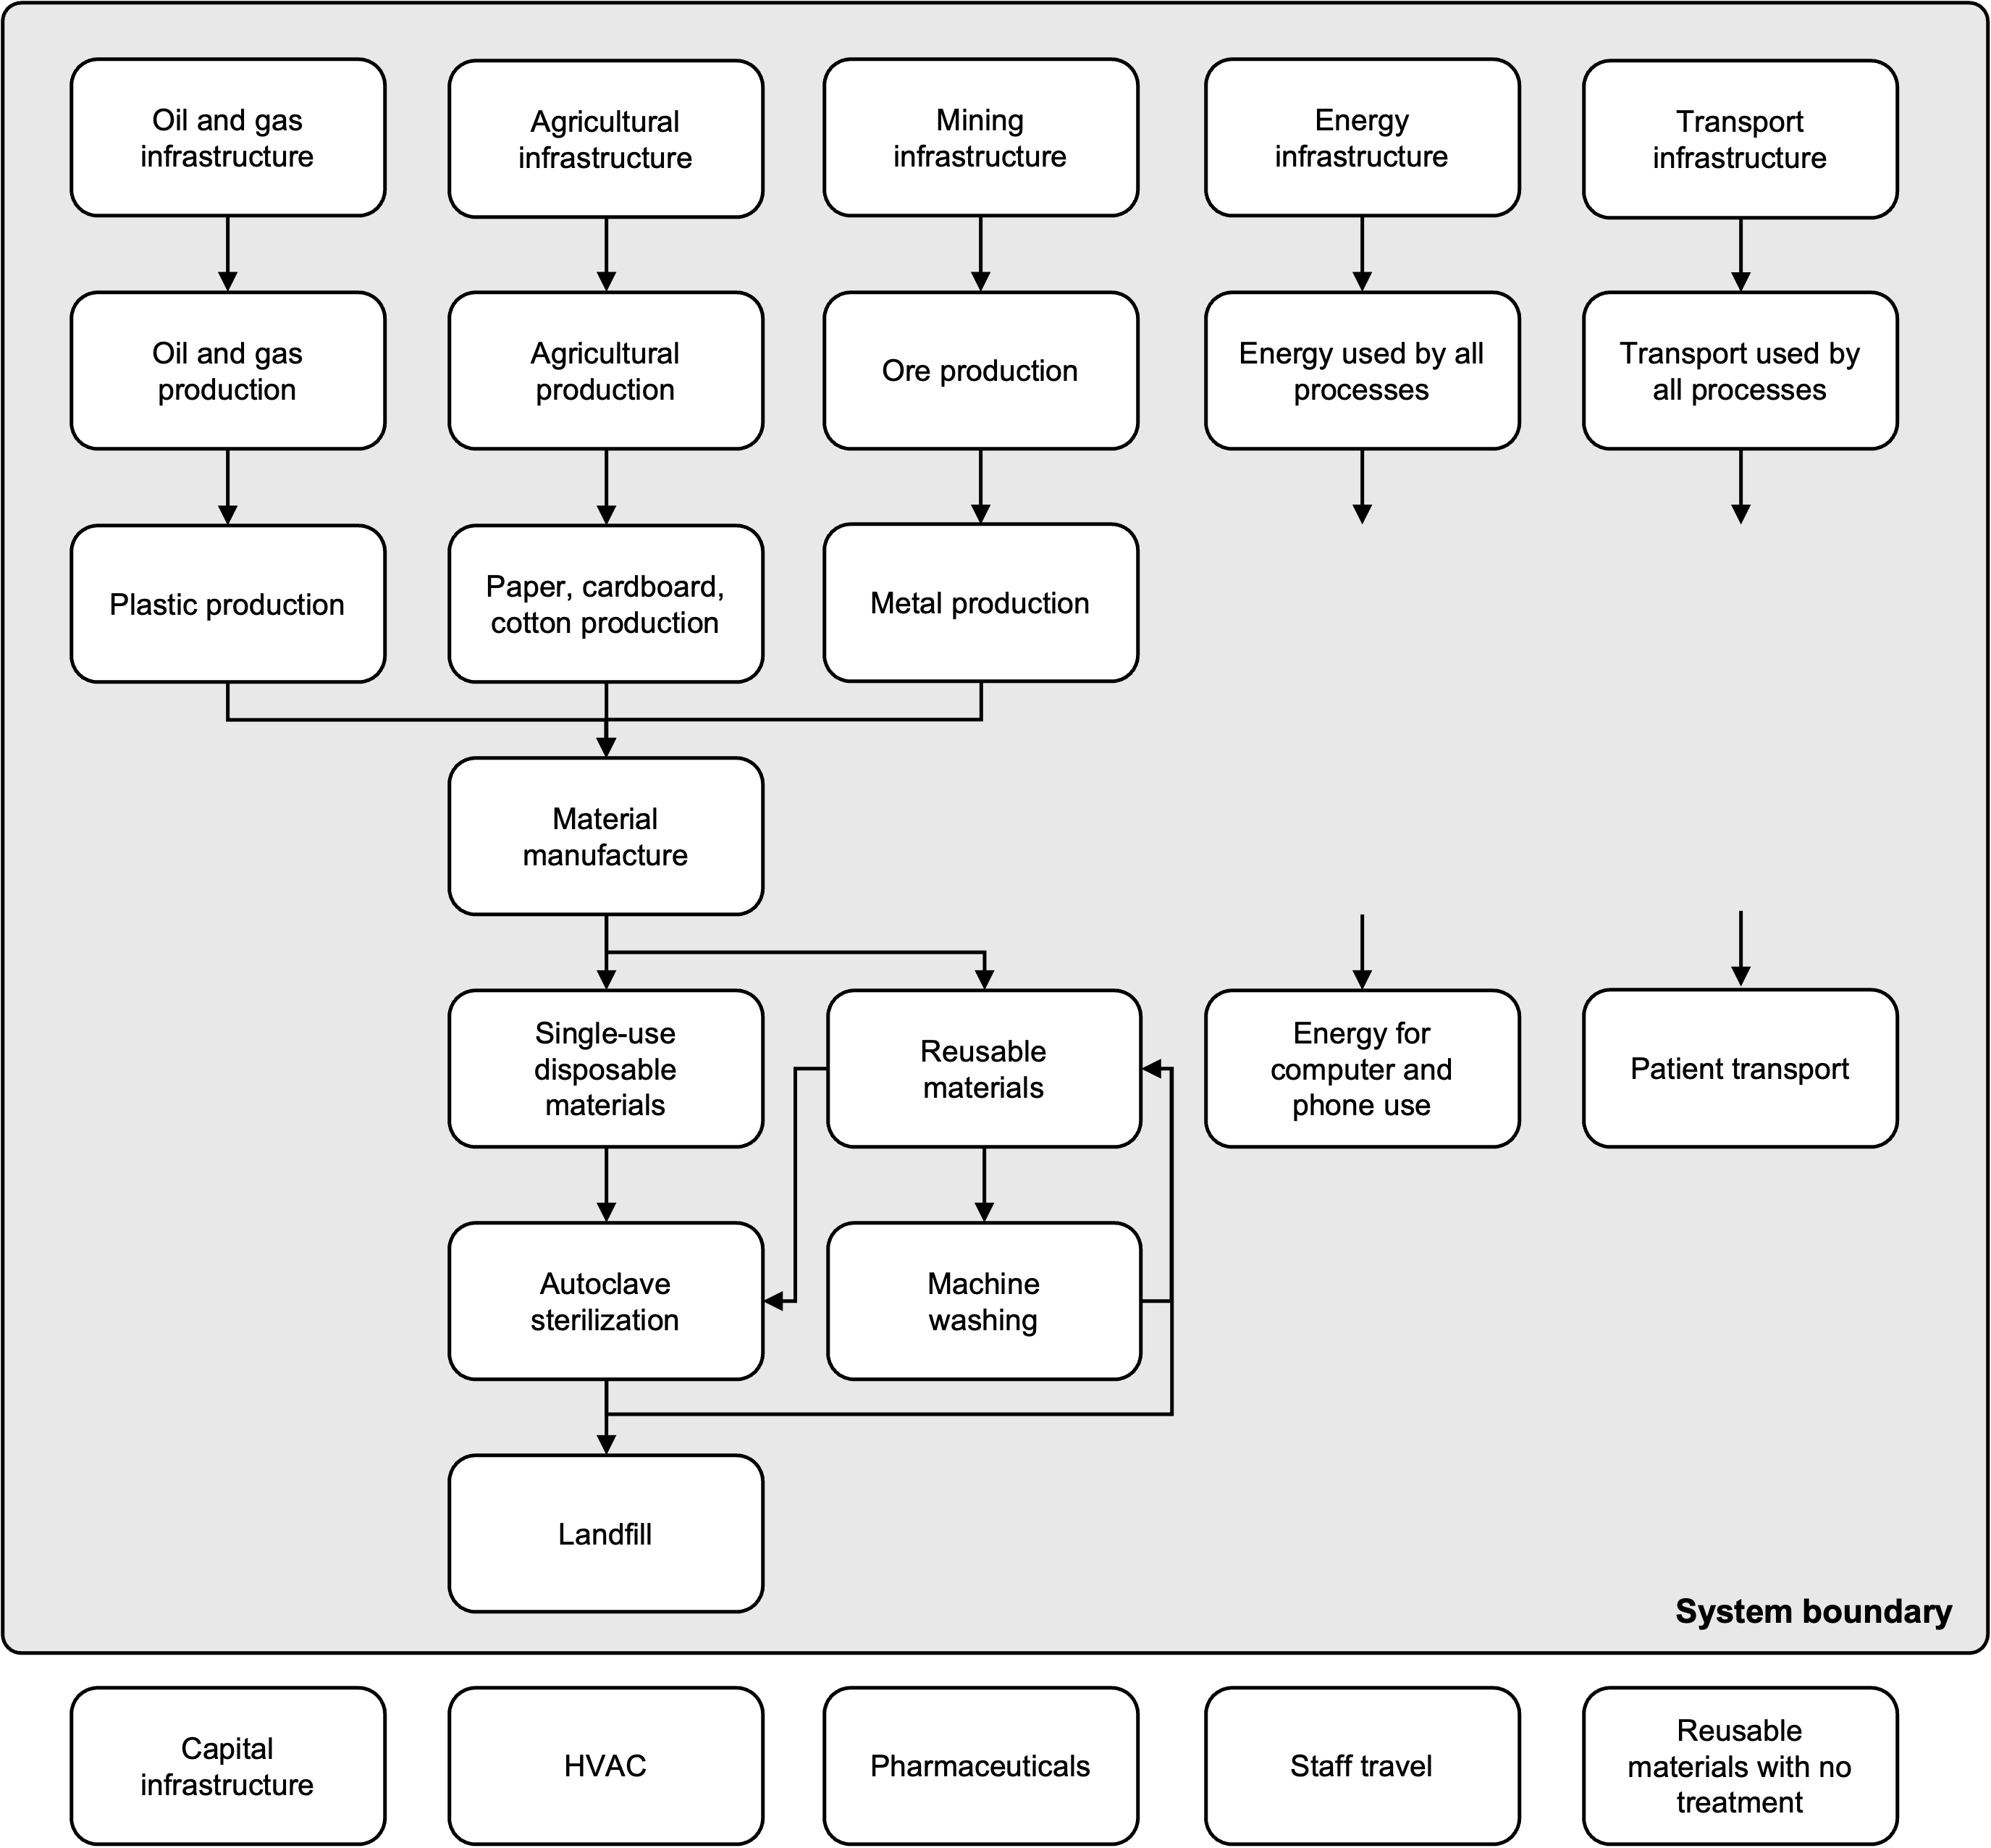
\includegraphics[width=1\linewidth]{core-chapters/figs/ch-6-fig-1.png}
    \caption{System boundary of the analysis.}
    \label{fig:ch-6-fig-1}
\end{figure}

\subsection{Study outcomes}
The primary outcome was greenhouse gas emissions in kilograms of carbon dioxide equivalent units (kg CO2-e). We included emissions from fossil, biogenic, and land use sources.

\subsection{Data collection}
Methods for data collection are provided in Supplementary Note 1. 

\subsection{Data analysis}
Data cleaning and analysis was conducted using R Version 4.4.3 and R Studio Version 2025. Life cycle assessment was modelled using SimaPro Analyst Release 9.6.0.1 (Pré Sustainability, Amersfoot, Netherlands). Background data on the environmental impact of processes were obtained from the AusLCI Version 2 (Lifecycles, Melbourne, Australia) database which uses background environmental data from Ecoinvent Version 3.10 (Ecoinvent, Zurich, Switzerland) databases. Impact assessment was modelled using the “IPCC 2021 GWP100” method (Version 1.03). Details and assumptions of modelling in SimaPro are provided in Supplementary Table 2. The primary outcome was reported for the entire functional unit, as well as for single use materials, reusable materials, electricity use, and patient travel.

\subsection{Subgroup analysis}
We undertook two subgroup analyses for emissions associated with appointments for surgical procedures. For the first, we compared emissions associated with the three types of surgical procedure for one lesion: excision, shave biopsy, and punch biopsy. For the second, we compared emissions for excision of one lesion versus multiple lesions during the same appointment. 

\subsection{Sensitivity analysis}
We conducted sensitivity analyses to determine the impact of different methods used to estimate patient travel (Supplementary Note 1). First, we excluded patients who travelled by plane to understand the impact of low-frequency but high-emission transport (details are provided in Supplementary Table 1). Second, transport emissions were halved to account for travel to two destinations on the same journey (e.g., if the patient drove to the clinic, had their appointment, went shopping, then went home). 

We conducted Monte Carlo simulations using 1,000 runs for all primary and subgroup analyses to estimate 95\% confidence intervals for greenhouse gas emissions. Monte Carlo simulation, conducted in SimaPro, uses random values within the probability distributions of inputs and outputs of all processes used in the study. We included all materials in this analysis, including those used during less than 50\% of observed appointments. Probability distributions of likely values for the number of materials used per appointment (single use and reusable), patient distance travelled, and appointment duration were modelled using either a triangular or log normal distribution. For triangular distributions, possible values were assumed to be between the minimum and maximum observed value. The most likely value was assumed to be the median. 

\section{Results}
Data collection by clinic is reported in Supplementary Table 3. Appointment length is reported in Supplementary Table 4. Material use is reported in Supplementary Tables 5-7 and materials included in the primary analysis are listed in Table 1. Details about the number and type of excisions performed during the excision appoints is reported in Supplementary Table 8. Material composition and weight is provided in Supplementary Table 9. Patient travel distance and mode of transport is reported in Supplementary Table 1. Material use for subgroup analyses are reported in Supplementary Tables 10-13. Material use for sensitivity analyses are reported in Supplementary Tables 1, 4, 5-7, 10, 12.

Greenhouse gas emissions associated with each functional unit are reported in Table 2. In all three functional units, patient transport was responsible for 10.72 kg CO2-e and was the greatest contributor to the total emissions (96\% for full skin examination, >99\% for total body photography, and 88\% for an excision of a lesion suspicious for melanoma) (Figure \ref{fig:ch-6-fig-2}). Total emissions were 11.11 kg CO2-e for a full skin examination, 10.75 kg CO2-e for total body photography, and 12.21 kg CO2-e for an excision of a lesion suspicious for melanoma. Emissions from single-use materials reflect the number and type of items included in the analysis (Table 1). For total body photography only single-use paper towels were included, and emissions were relatively low (0.01 kg CO2-e). For excisions, 18 single-use (e.g., gauze, suture, gloves) and four reusable (e.g., scissors, needle holder, scalpel handle) materials were included, and emissions were relatively high (1.26 kg CO2-e). Emissions from energy use was low across all three functional units. 

\begin{figure}
    \centering
    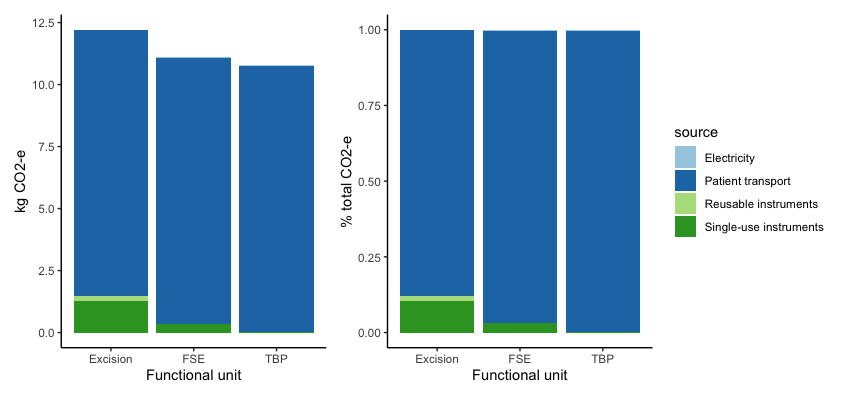
\includegraphics[width=1\linewidth]{core-chapters/figs/ch-6-fig-2.png}
    \caption{Greenhouse gas emissions of full skin examination, total body photography, and excision of a lesion suspicious for melanoma, by source of emission.}
    \label{fig:ch-6-fig-2}
\end{figure}

Subgroup analyses found slightly lower total emissions for shave biopsy than other excision types (12.20 kg CO2-e for one excision biopsy, 13.65 kg CO2-e for one punch biopsy, and 11.36 kg CO2-e for one shave biopsy), and a modest increase for >1 concurrent excisions (11.72 kg CO2-e for one lesion and 12.43 kg CO2-e for more than one lesion). These differences were largely explained by variation in emissions from single use instruments between subgroups. These were higher for excision biopsies (1.25 kg CO2-e) than for punch (0.97 kg CO2-e) and shave (0.64 kg CO2-e) biopsies, and for appointments with more than one lesion removed (1.48 kg CO2-e) than for appointments with only one lesion removed (0.82 kg CO2-e). Details are reported in Supplementary Table 14. 

Sensitivity analyses found emissions from patient travel reduced from 10.72 to 9.69 kg CO2-e when travel by plane was excluded (n=2/262; 0.8\%), and to 5.36 kg CO2-e when an additional destination was assumed to occur on the dermatology clinic journey. Emissions reduced to 4.85 kg CO2-e when both were true (i.e., plane travel was excluded and an additional destination was assumed to occur on the journey). The results of the primary analysis were highly sensitive to the methods used to calculate emissions from patient transport.

Monte Carlo simulations showed large uncertainties. Confidence intervals (95\%) for total GHG emissions (kg CO2-e) were 1.93 – 55.53 for full skin examination, 1.60 – 54.54 for total body photography, and 2.92 – 61.58 for excision. Probability distributions of the Monte Carlo simulations were skewed and followed a log normal pattern. Full results of Monte Carlo simulations are reported in Supplementary Table 15.

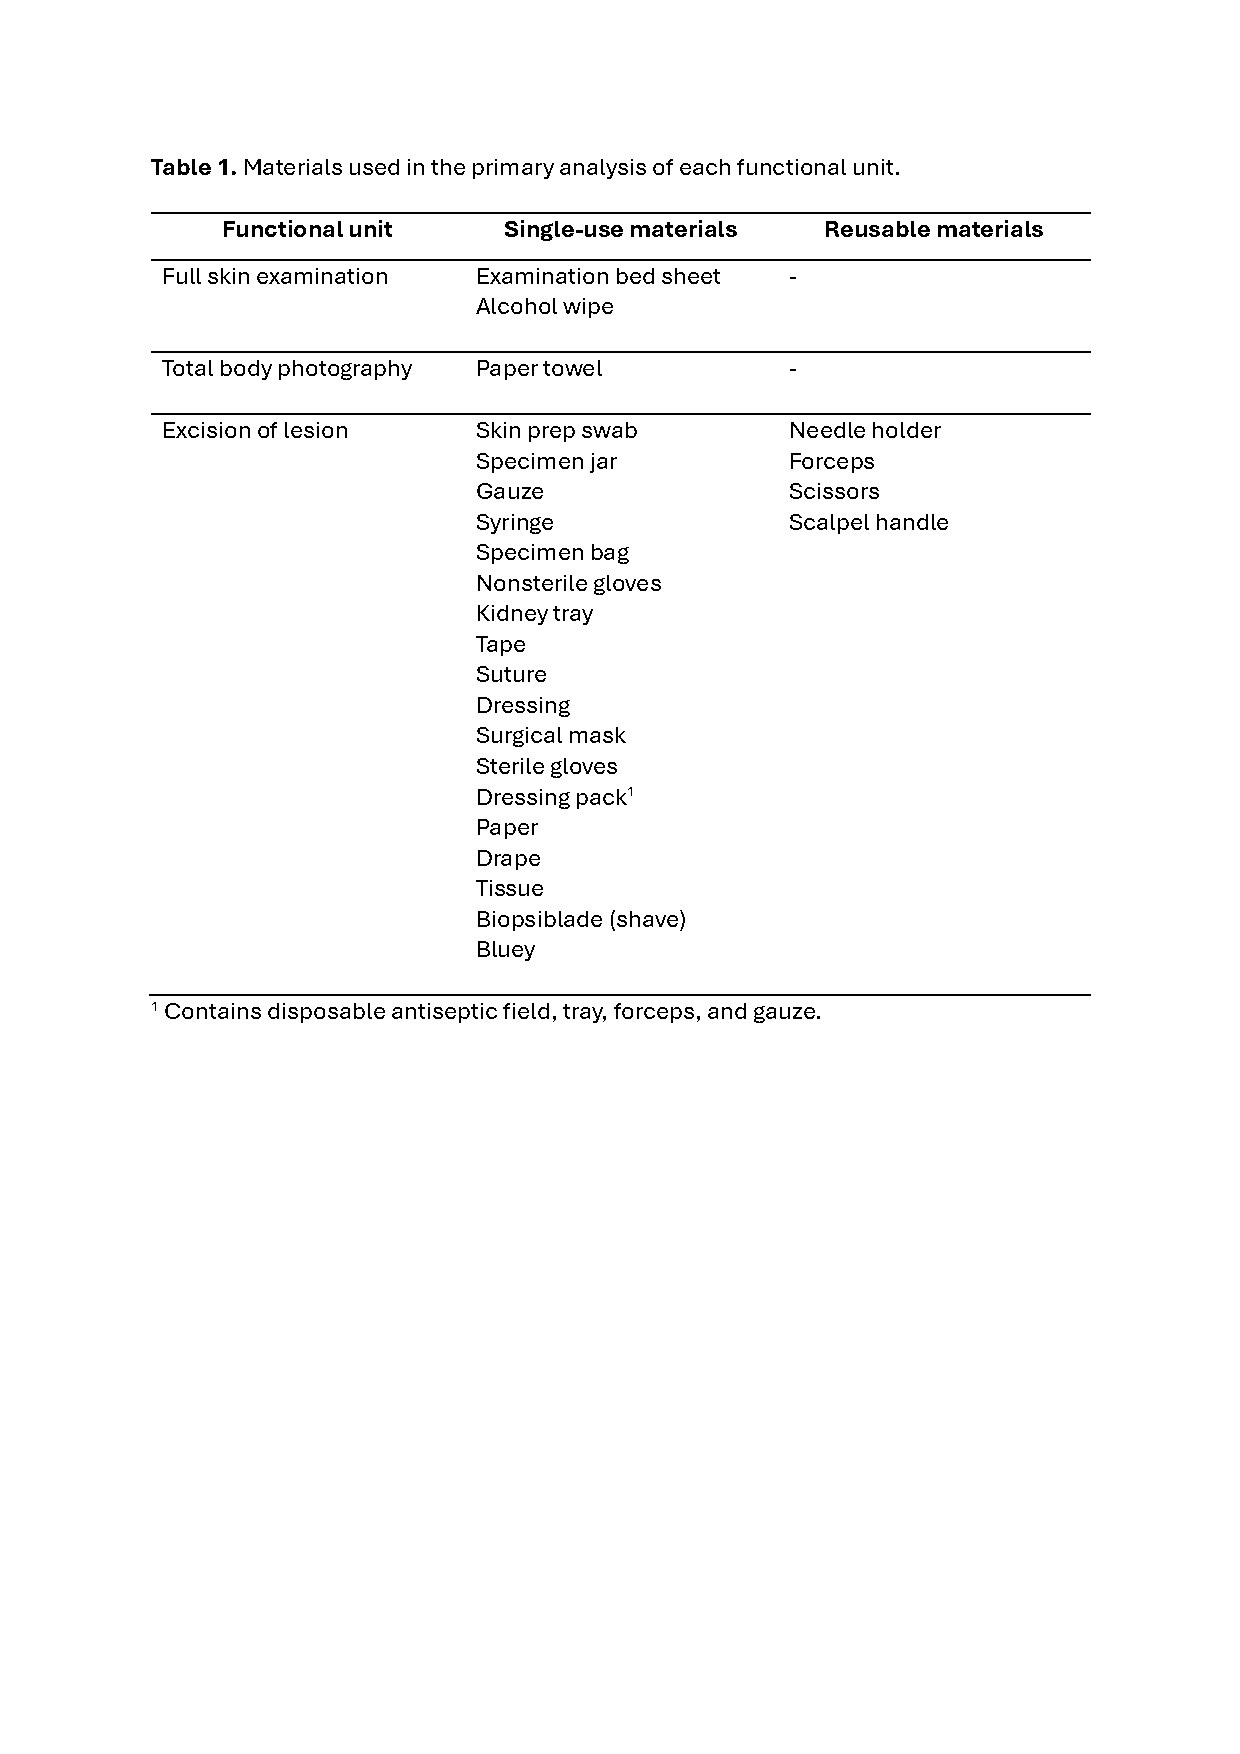
\includepdf[]{core-chapters/ch-6-tab-1.pdf}
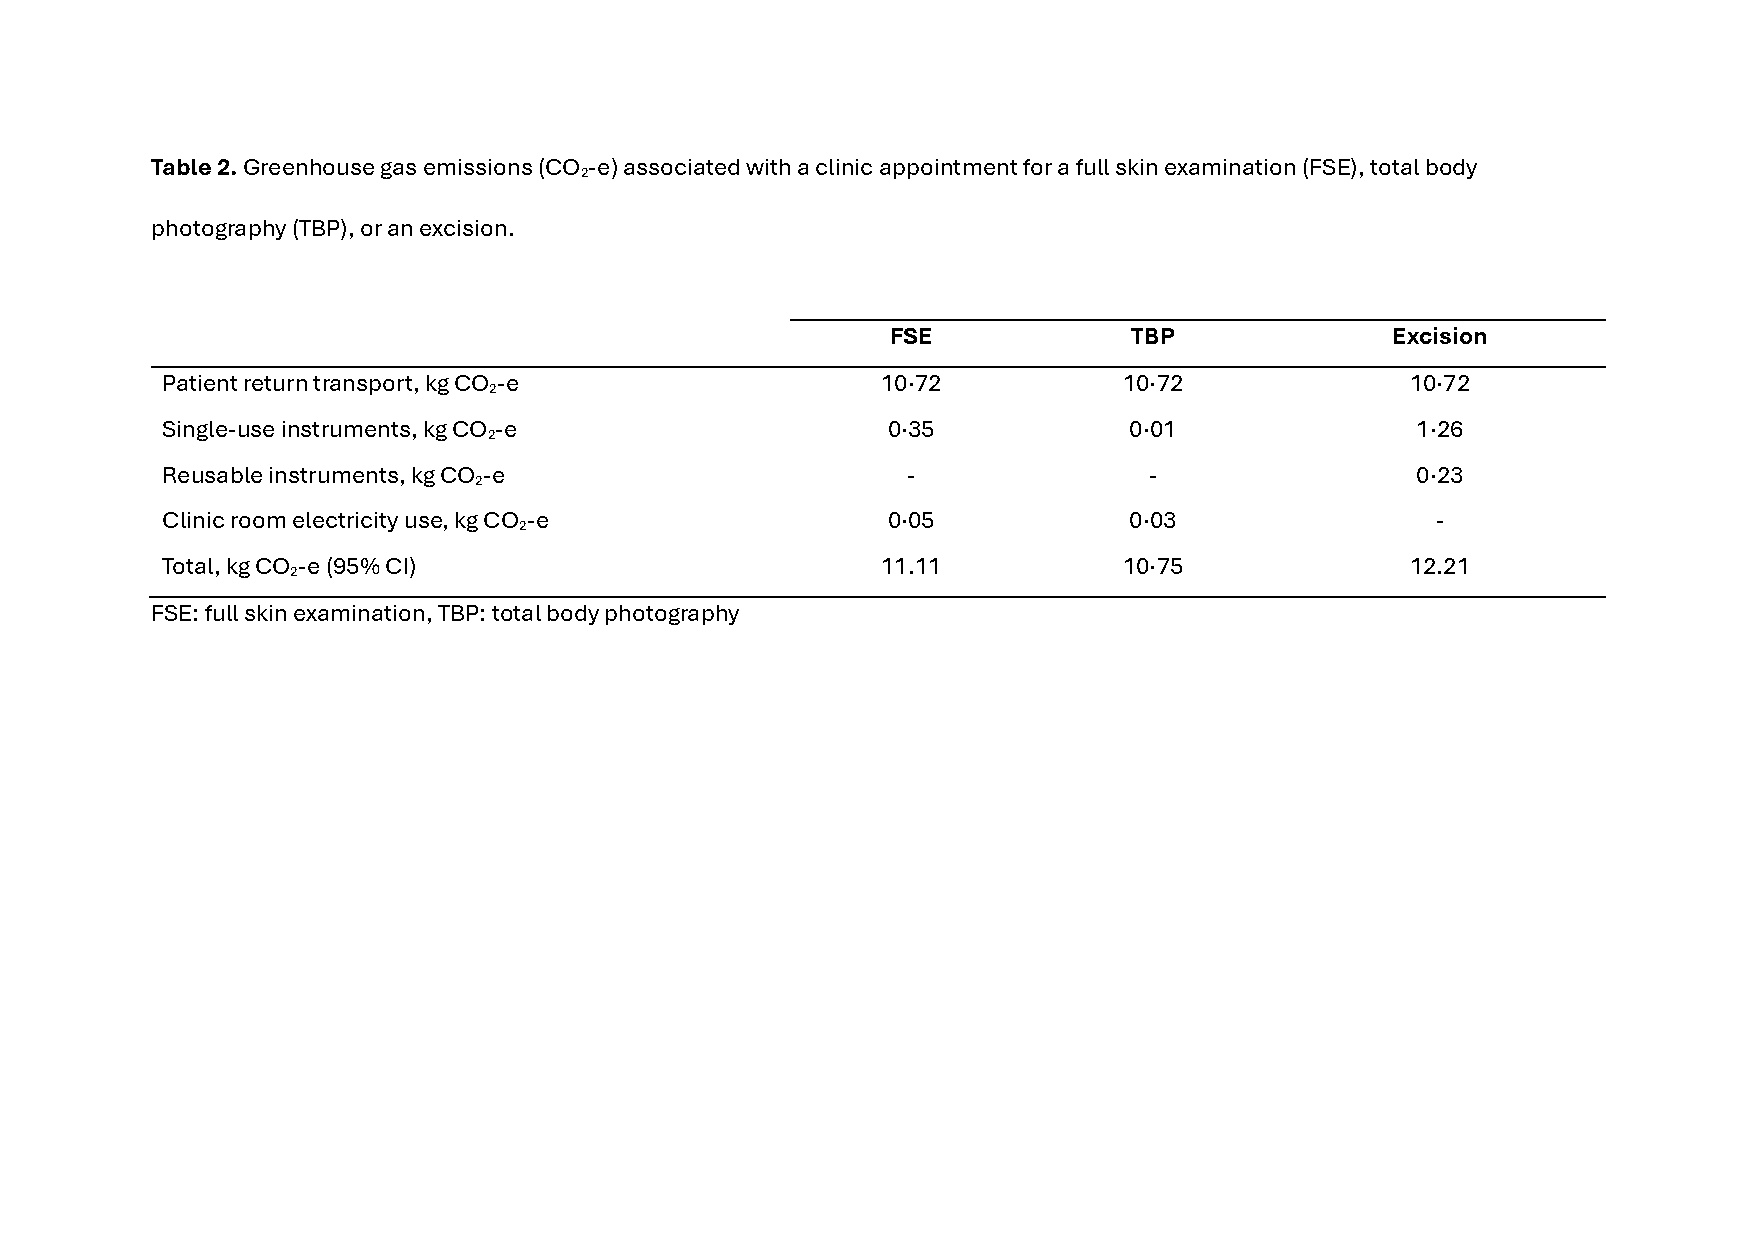
\includepdf[landscape=true]{core-chapters/ch-6-tab-2.pdf}

\section{Discussion}

This study reports the carbon emissions associated with an appointment for a full skin examination, total body photography, and an excision of a lesion suspicious for skin cancer. Emissions were similar between the three activities and ranged between 10.75 kg and 12.21 kg CO2-e. Among surgical appointments, total emissions were similar for different types of procedure (excision biopsy, punch biopsy, shave biopsy) and for the number of lesions removed in a single appointment (one lesion, more than one lesion). 

In all three functional units carbon emissions were driven by patient transport, which accounted for 88\% to more than 99\% of emissions in the primary analyses. Single-use and reusable materials accounted for less than 1\% of total emissions in the non-surgical functional units and 13\% in the surgical functional unit, reflecting the higher number of materials used during excisions of the skin than in full skin examinations and total body photography. Monte Carlo simulations suggest the findings of this study are uncertain with point estimates having large confidence intervals. Still, it highlights the importance of patient transport as a key component of the carbon emissions associated with clinical dermatology care. Patient transport is likely to be important for clinical appointments for other conditions in which a small number of materials are consumed, such as non-surgical general practice or specialist consultations. Our findings are consistent with those from a recent review that, when included, patient travel has relatively large contributions to the carbon emissions of hospital services and care pathways.\cite{kouwenberg_carbon_2024}

Only a few studies have investigated the carbon emissions of skin cancer dermatology care globally. Recent studies estimated the annual emissions of a large dermatology practice in the United States (324 t CO2-e per year)\cite{silva_carbon_2025} and emissions for different melanoma follow-up guidelines in the United Kingdom (ranging between 166 kg and 316 kg CO2-e per person per year).\cite{grover_relative_2024} Another study estimated emissions of hypothetical virtual compared to in-person review of a skin lesion in Aotearoa New Zealand, reporting 11 kg CO2-e fewer emissions per appointment in hypothetical virtual follow-up.\cite{jones_virtual_2024} These studies provide some context to our results but are not based on the findings of full process-based life cycles assessments. As with all studies of carbon emissions, the conclusions drawn depend on the scope of the analysis. For example, in the US study by Silva et al. purchased goods and services were the dominant source of emissions,\cite{silva_carbon_2025} whereas in our analysis patient transport dominated the results.

There are two existing process-based LCA in this field, one for the surgical removal of a skin cancer in a dermatology clinic in Australia and one for non-melanoma skin cancer surgery in a specialist plastic surgery centre in Wales.\cite{tan_carbon_2021, ang_carbon_2024} 

The Australian study, by Tan \& Lim, reports carbon emissions of 29 kg CO2-e per excision, approximately triple our finding but within our 95\% confidence interval estimate for this functional unit (2.92 – 61.58 kg CO2-e per appointment). This difference is partly attributable to differences in system boundaries and modelling assumptions between the two studies. This is common in life cycle assessment research. Notably, Tan \& Lim included staff travel within their system boundary, which was excluded from this study, and empirical data for mode of transport and distance travelled was not used. Another difference relates to the transportation of materials to and from the clinic. Tan \& Lim estimate this to be about 8.6 kg CO2-e per appointment, compared to our estimate of 1.5 kg CO2-e for total emissions from the full material life cycle (including transportation to and from the clinic and all other stages of the life cycle). The drivers of this difference are difficult to determine with certainty. One possible explanation is a difference in the way emissions from transport of materials to and from the clinic were included. Specifically, whether emissions were included based on the total vehicle distance travelled (e.g., emissions per kilometre), or on the proportion of those emissions attributable to the weight of the relevant items carried by that vehicle (e.g., emissions per gram-kilometre), which was often only a few grams per item (see Supplementary Table 7).

It is important to note that the scenarios investigated in this study are not substitutable and have different purposes. A full skin examination has a different purpose to an excision of a lesion or total body photography, and emissions reductions cannot be estimated between the functional units. Even within the surgical functional unit, clinical practice guidelines recommend the use of excision, punch, and shave biopsies for different purposes, and while emissions may be (non-significantly) lower for shave excisions, it would be incorrect to recommend this procedure in the context of a lesion suspicious for melanoma.\cite{adler_methods_2019}

Despite this, there are opportunities for clinical practice to reduce carbon emissions based on the findings of this study. An existing review of sustainable dermatological surgery made several recommendations to reduce emissions, and these should be implemented where it is safe to do so.\cite{ali_environmental_2025, ali_environmental_2025-1} The findings of this study suggest that most emissions from clinic appointments are attributable to patient transport and therefore reducing the need for this transport will have the greatest impact. Previous studies of emissions from healthcare services have therefore encouraged the use of carpooling, public transport, and cycling in an effort to reduce these emissions.\cite{tan_carbon_2021, barraclough_carbon_2025} Emissions from patient transport can also be reduced by performing multiple procedures or investigations on the same day wherever clinically acceptable, for example by performing a full skin examination and an excision during the same visit instead of in two separate visits. This reduces emissions from 23.32 to 12.6 kg CO2-e (Table 1). While all these actions may be effective, clinicians seeking to reduce emissions should focus on reducing the need for patients to visit the clinic in the first place where this is clinically appropriate, such as by reducing unnecessary excisions and appointments.

Healthcare overuse is a well described problem in modern medicine and is associated with harms to the patient, practitioner, public, and planet.\cite{gram_less_2025} These harms include carbon emissions, such as those described in this study, which are emitted without any health benefit to the patient.\cite{barratt_high_2022} While the issue of overdiagnosis was not explored directly in this study, previous work suggests that the overdiagnosis of melanoma may be common, especially for in-situ melanoma in patients who have had full skin examinations, which results in cascades of subsequent care and a higher rate of healthcare use and environmental impacts with no health benefit to the patient.\cite{bell_melanoma_2022} Some full skin examinations, total body photographs, or excisions are likely unnecessary, and limiting these is an effective way to reduce emissions. This could include tailoring services according to need by adopting a risk-based approach to screening and surveillance (FSE and TBP) and using new technologies to monitor lesions and reduce unnecessary skin excisions,\cite{pellacani_effect_2022, smith_implementing_2024} including the possibility of remote monitoring.\cite{drabarek_perspectives_2022} This is of particular importance in Australia given the recently announced roadmap for a targeted national skin cancer screening program, and its equity objectives of providing access to screening regardless of where a person lives.

This study has several strengths. First, we used process-based life cycle assessment methodology to estimate carbon emissions across the entire life cycle of all processes included in this study. Process-based LCAs are the most accurate way to estimate carbon emissions at the level of a single healthcare activity. Second, we collected and used empirical data about materials and patient transport and did not rely on estimates for these parts of our analysis. This is especially beneficial for patient transport because it accounted for such a large proportion of emissions. Previous studies made assumptions about distance travelled and modality of transport.\cite{tan_carbon_2021}

The primary limitation of this study is that it is based on data collected from two Australian metropolitan specialist clinics in Sydney and this is likely to impact on the distance travelled and modality of transport used by patients. This means our findings may not be applicable to other parts of Australia, particularly regional and small community practices where transportation is likely to be very different. It may also not be applicable to some international contexts with higher proportions of patients using public transport and smaller distances for those who drive. Parts of our model are based on assumptions and data that was not directly measured. This included assuming shipping and road-transport distances from the manufacturer of materials to the clinic, and transport from the clinic to sterilisation and landfill sites. We also excluded several processes on the basis that their emissions were likely to contribute less than 1\% of emissions. Emissions from the pathological review of excised skin lesions was excluded, as were emissions from all the cascaded care that follows a melanoma diagnosis.

This study found carbon emissions associated with dermoscopy-guided full skin examination, total body photography, and the excision of a lesion suspicious for melanoma or keratinocytic cancer were similar and almost exclusively driven by patient transport. Emissions reductions can be achieved by reducing the need for patients to visit the clinic, where this is safe to do so.


\printbibliography[heading=subbibliography]
\end{refsection}

\chapter{Methods to include environmental impacts in a cost-effectiveness analysis: a case study of surveillance imaging after treatment for stage III melanoma}
\label{ch-7}

The aim of this chapter was to demonstrate methods to include carbon emissions in a cost-effectiveness analysis of different PET/CT surveillance imaging schedules for detecting distant metastasis after treatment for stage III melanoma. It was published in \textit{Value in Health}. Supplementary material are provided in Appendix \ref{ap-g}.

\paragraph*{Publication details}
\textit{Williams JTW}, Bell KJL, McAlister S, Morton RL. Methods to include environmental impacts in a cost-effectiveness analysis: a case study of surveillance imaging after treatment for stage III melanoma. Value in Health. In press.

% PDF of published paper
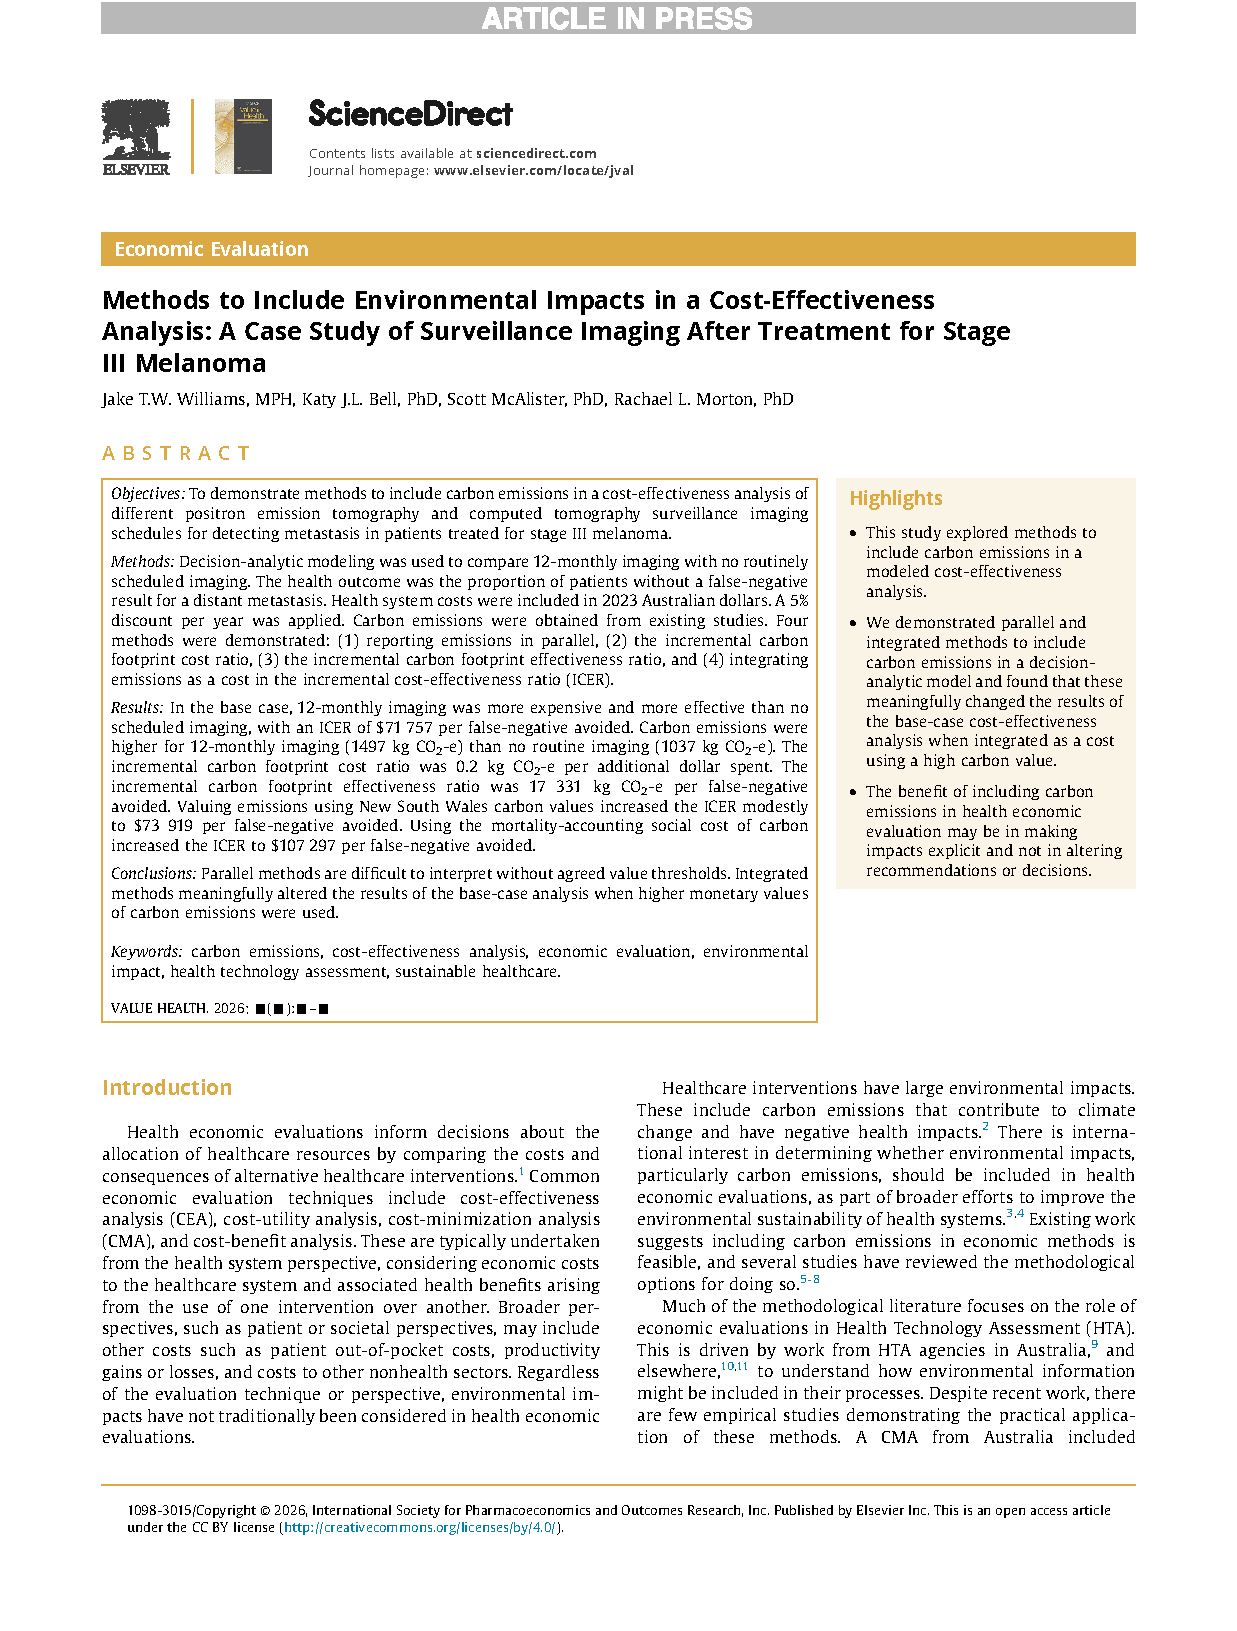
\includepdf[
  pages=1,
  pagecommand={
    \thispagestyle{empty}
    \addcontentsline{toc}{section}{\numberline{7.1}Abstract}
    \addcontentsline{toc}{section}{\numberline{7.2}Highlights}
    \addcontentsline{toc}{section}{\numberline{7.3}Introduction}
  }
]{pdfs/ch-7.pdf}

\includepdf[
  pages=2,
  pagecommand={
    \thispagestyle{empty}
    \addcontentsline{toc}{section}{\numberline{7.4}Methods}
  }
]{pdfs/ch-7.pdf}

\includepdf[
  pages=3,
]{pdfs/ch-7.pdf}

\includepdf[
  pages=4,
]{pdfs/ch-7.pdf}

\includepdf[
  pages=5,
  pagecommand={
    \thispagestyle{empty}
    \addcontentsline{toc}{section}{\numberline{7.5}Results}
    \addcontentsline{toc}{section}{\numberline{7.6}Discussion}
  }
]{pdfs/ch-7.pdf}

\includepdf[
  pages=6,
]{pdfs/ch-7.pdf}

\includepdf[
  pages=7,
  pagecommand={
  \thispagestyle{empty}
    \addcontentsline{toc}{section}{\numberline{7.7}References}
  }
]{pdfs/ch-7.pdf}

\includepdf[
  pages=8,
]{pdfs/ch-7.pdf}
\chapter{Towards Environmentally Extended Health Economic Analysis Plans: A Case Study for the MEL‑SELF Trial}
\label{ch-8}

The aim of this chapter was to outline items we include in a health economic analysis plan (HEAP) for the economic evaluation of the MELanoma SELF surveillance (MEL-SELF) randomised controlled trial. It was published in \textit{Applied Health Economics and Health Policy}. The supplementary material is Version 1.0 of the MEL-SELF HEAP and is provided in Appendix \ref{ap-h}. The HEAP was also published on the \textit{Open Science Framework}.

\paragraph*{Publication details}
\textit{Williams JTW}, Bell KJL, McAlister S, Morton RL. Towards Environmentally Extended Health Economic Analysis Plans: A Case Study for the MEL-SELF Trial. Applied Health Economics and Health Policy. In press.

% PDF of published paper
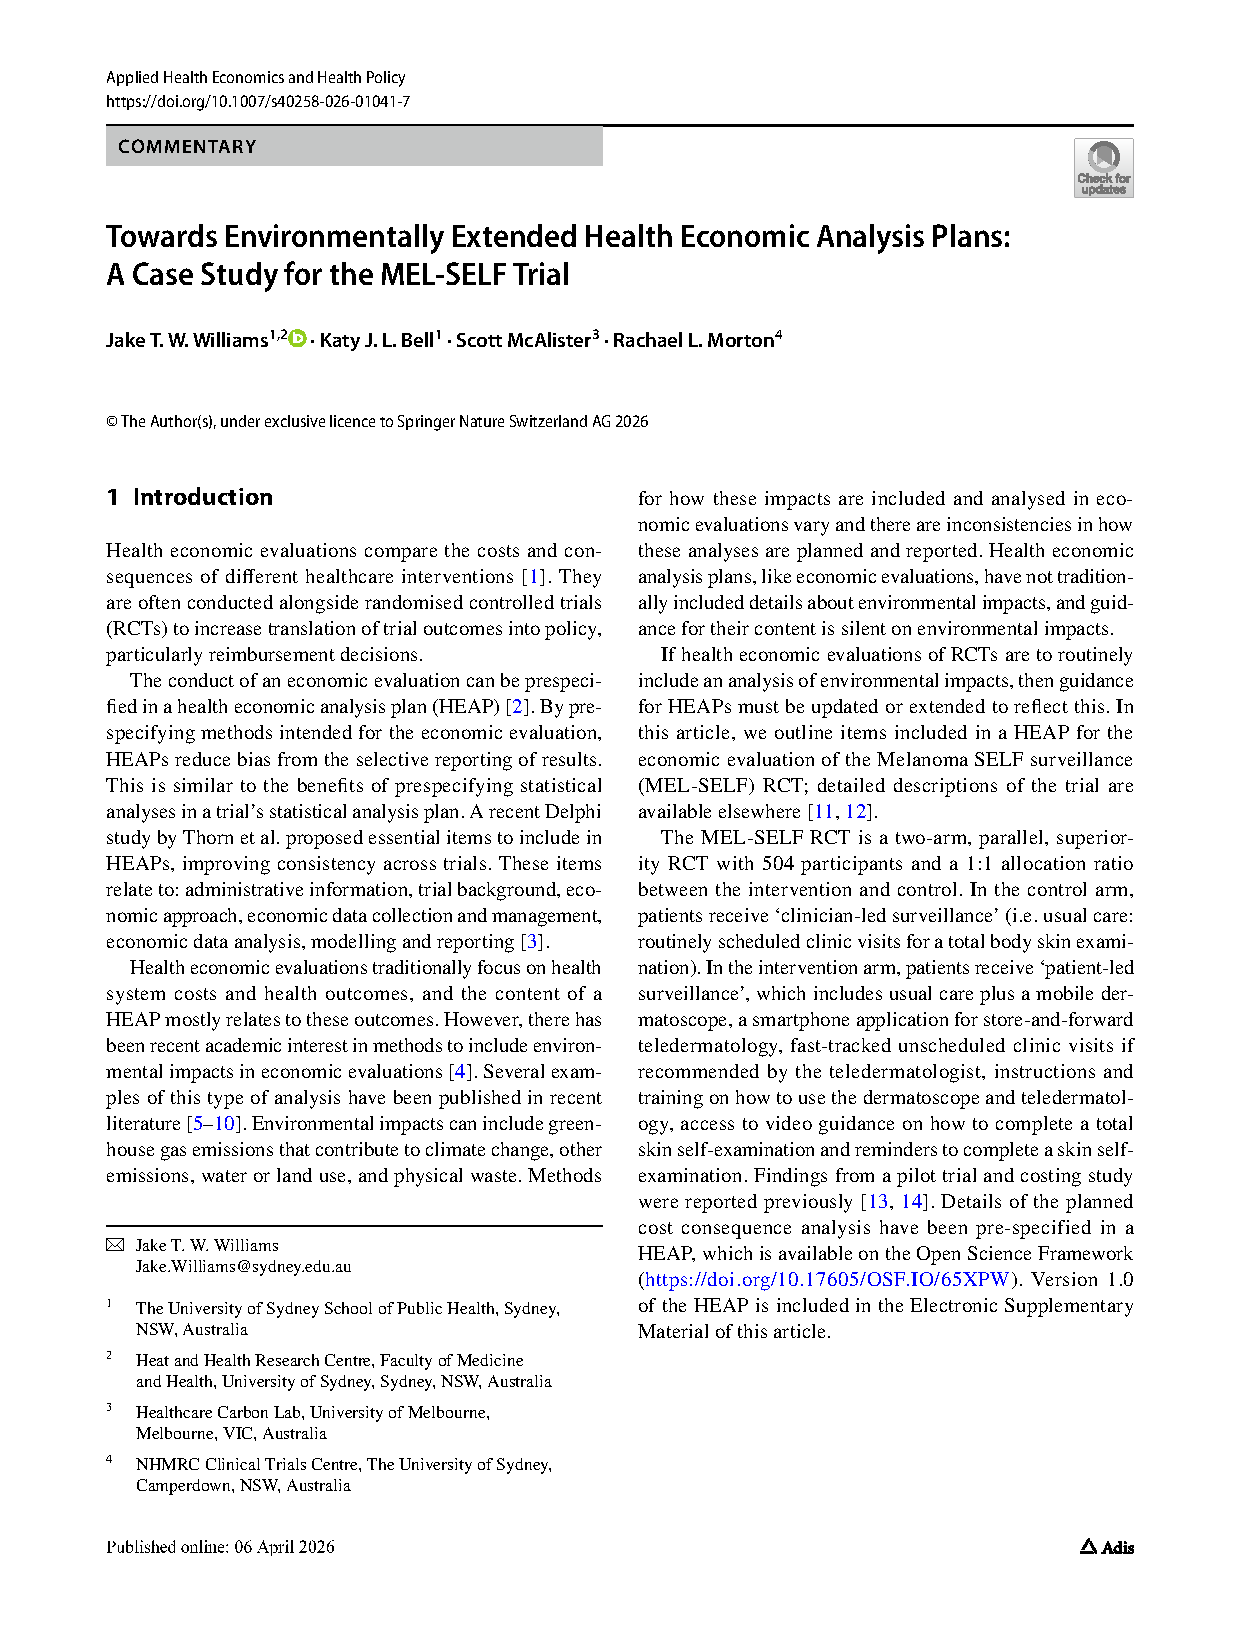
\includepdf[
  pages=1,
  pagecommand={
    \thispagestyle{empty}
    \addcontentsline{toc}{section}{\numberline{8.1}Introduction}
  }
]{pdfs/ch-8.pdf}

\includepdf[
  pages=2,
  pagecommand={
    \thispagestyle{empty}
    \addcontentsline{toc}{section}{\numberline{8.2}Items for and Environmentally Extended HEAP}
    \addcontentsline{toc}{section}{\numberline{8.3}Discussion}
  }
]{pdfs/ch-8.pdf}

\includepdf[
  pages=3,
]{pdfs/ch-8.pdf}

\includepdf[
  pages=4,
]{pdfs/ch-8.pdf}

\includepdf[
  pages=5,
]{pdfs/ch-8.pdf}

\includepdf[
  pages=6,
  pagecommand={
    \thispagestyle{empty}
    \addcontentsline{toc}{section}{\numberline{8.4}References}
  }
]{pdfs/ch-8.pdf}
\chapter{Methods to include environmental impacts in Australian health technology assessment}
\label{ch-9}

\begin{refsection}[refs/ch-9.bib]

The aim of this chapter was to outline the current Australian policy context for including environmental impacts in health technology assessment, evaluate potential methods to include environmental impacts in HTA for public reimbursement, and detail a method for use in the cost-minimisation pathway. This chapter contains the same text as a manuscript being prepared for submission. It summarises previous chapers for a policy audience and is partially based on concepts developed for an Issues Brief published by the Deeble Institute for Health Policy Research, which is provided in Appendix \ref{ap-i}.

\paragraph*{Publication details}
Manuscript authored by Jake T W Williams, Katy J L Bell, Scott McAlister, Madeleine Skellern, Rebecca Haddock, and Rachael L Morton. It is being prepared for submission.

\clearpage

\section{Introduction}
Health technology assessment (HTA) is a multidisciplinary process used in health systems to evaluate new health technologies including pharmaceuticals, tests, devices, vaccines, procedures, programs, or systems. The objective of HTA is to ensure new technologies provide health (or other) benefits at a cost acceptable to society.\cite{orourke_new_2020} In Australia, HTA is used to inform decisions about whether a new technology should receive publicly funded reimbursement, and environmental impacts are not currently considered during this process. However, there is interest in understanding if this should be done and how it could be implemented. The aim of this article is to: (1) outline the current Australian policy context relevant for including environmental impacts in HTA; (2) evaluate potential methods to include environmental impacts in Australian HTA for public reimbursement; and (3) detail one potential method for the Australian cost-minimisation pathway. 

\section{Australian Health Technology Assessment}
HTAs conducted globally usually include assessments of the technology’s safety, efficacy, clinical effectiveness, cost-effectiveness, and affordability; and may include other factors such as patient, caregiver, and clinician acceptability , health equity, ethical issues, and feasibility of implementation.\cite{world_health_organization_2015_2015} They do not currently consider environmental impacts. 

In Australia, most funding for healthcare comes from government sources, and two thirds of this comes from the Commonwealth Government.\cite{australian_institute_of_health_and_welfare_health_2024} While healthcare is also funded at other levels of government (e.g., by states and territories) and by individuals and households (e.g., for private services that do not receive reimbursement), HTA is used most prominently by the Commonwealth Government to inform decisions about which technologies are subsidised through one of Australia’s universal access schemes, such as the Pharmaceutical Benefits Scheme (PBS) or Medicare Benefits Schedule (MBS), as well as the level of the reimbursement provided. HTAs for this purpose are notably evaluated by the Pharmaceutical Benefits Advisory Committee (PBAC) and Medical Services Advisory Committee (MSAC). Guidelines for HTA submitted by applicants to MSAC for evaluation explicitly permit environmental impacts to be considered (Box 1),\cite{australian_government_department_of_health_disability_and_ageing_guidelines_2021} but this is not a requirement and it is unknown how often this information is submitted as part of an application. HTA submitted by applicants to the PBAC do not explicitly permit environmental impacts to be considered.\cite{australian_government_department_of_health_disability_and_ageing_guidelines_2016}

The Commonwealth Government is considering reforms to Australia’s HTA processes in response to the Health Technology Assessment Policy and Methods Review (henceforth HTA Review), published in 2024.\cite{australian_government_department_of_health_and_aged_care_health_2024} The HTA Review’s final report included a recommendation (Recommendation 43) to investigate options to include environmental impacts in HTA processes. This recommendation built on a related commitment in the 2023 National Health and Climate Strategy (Box 1).\cite{australian_government_department_of_health_and_aged_care_national_2023} The broader HTA policy context therefore presents a timely opportunity for Australia to progress this work. There is also international interest in this topic, with HTA bodies in the United Kingdom and Canada exploring ways to include environmental impacts in HTAs conducted in their health systems (Box 2). Despite this recent work, no jurisdiction routinely considers environmental impacts during HTA. 

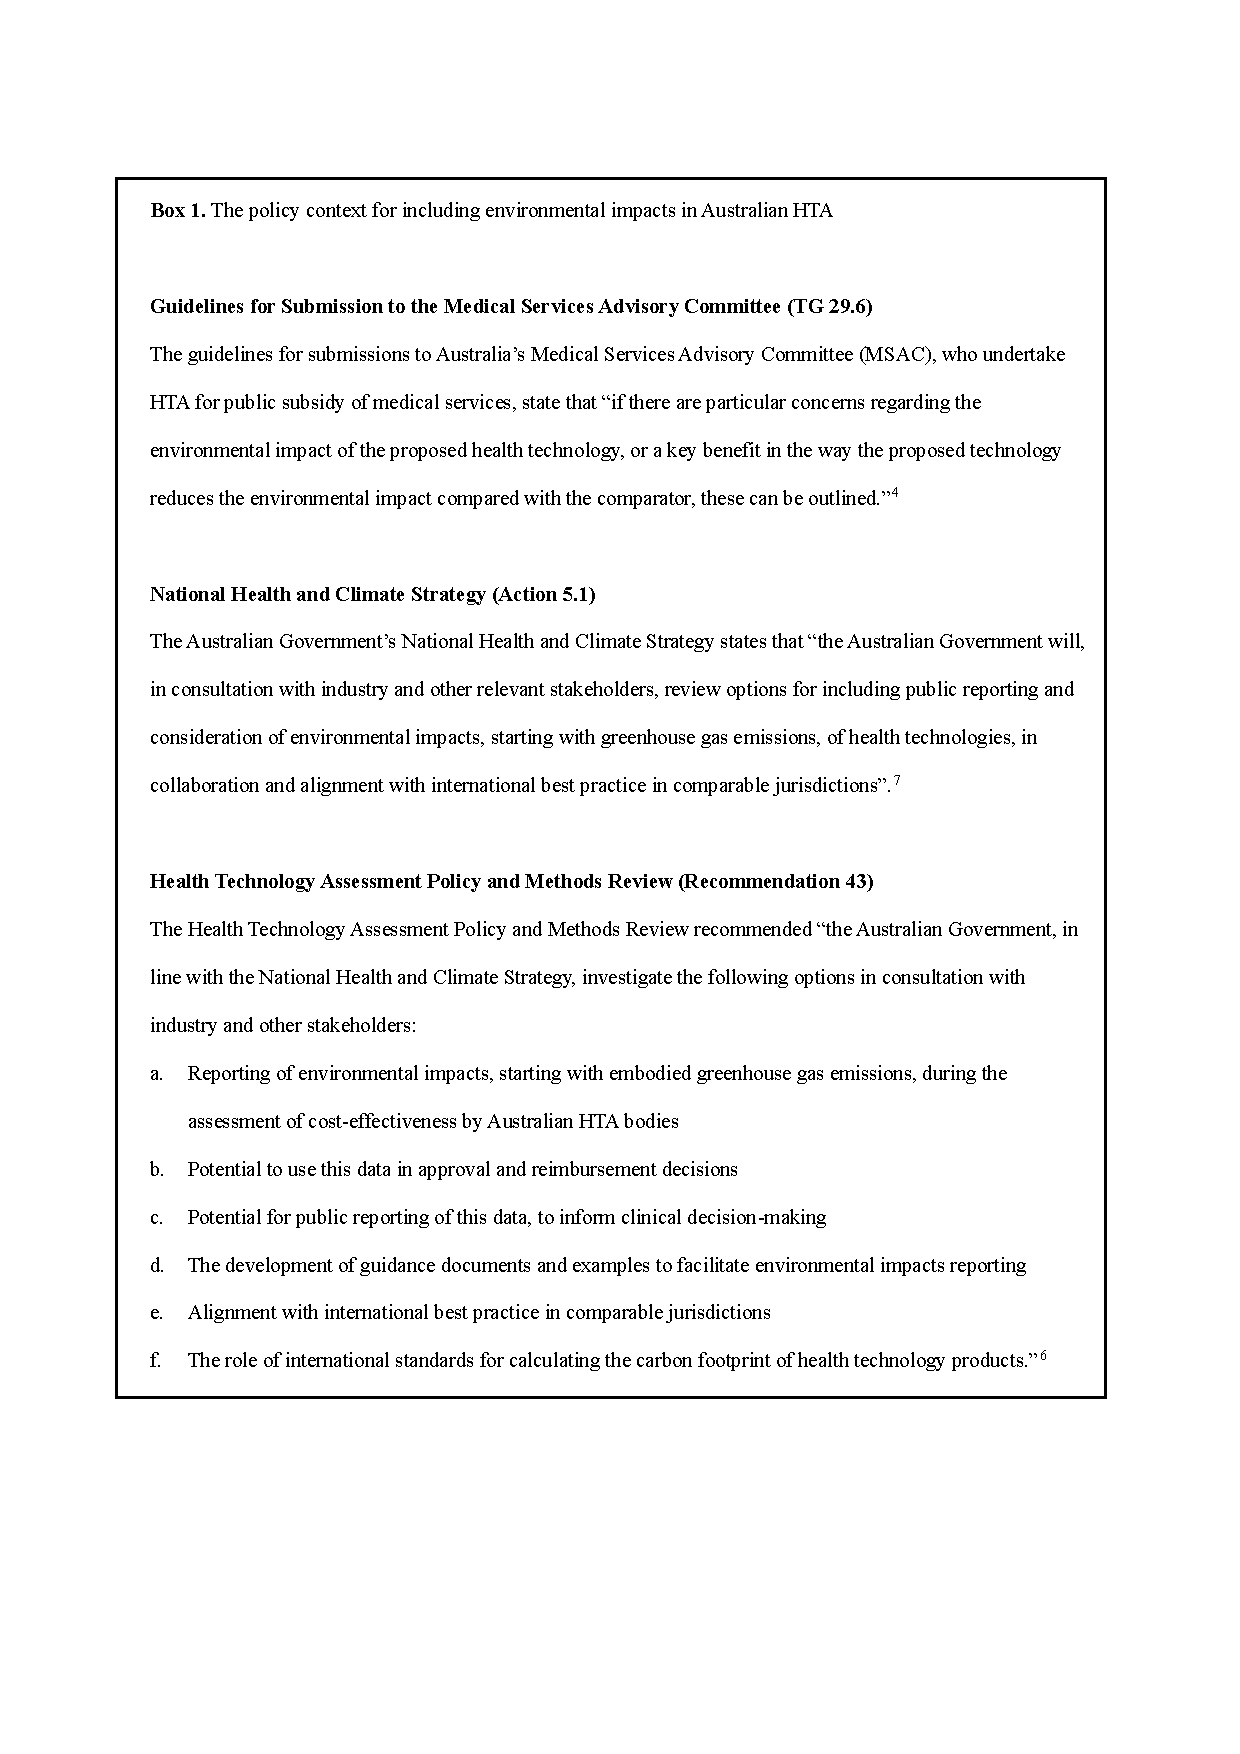
\includepdf[pages=-]{core-chapters/ch-9-box.pdf}

\section{Methods to include environmental impacts in HTA}
There is a growing literature dedicated to identifying, describing, and evaluating methods to include environmental impacts in HTA.\cite{guirado-fuentes_main_2023, toolan_environmental_2023, marsh_expanding_2016, desterbecq_inclusion_2023, mcalister_incorporating_2022, pinho-gomes_incorporating_2022, williams_methods_2024, ardito_which_2025} In this section we outline four broad methods and evaluate their potential use in Australia: (1) information conduit, (2) integrated evaluation, (3) parallel evaluation, or (4) environment-focused evaluation.\cite{toolan_environmental_2023}

\subsection{Information conduit}
An information conduit approach proposes the collection and publication of environmental impact data, but without using these data in the approval and reimbursement decision-making process. The applicant would submit environmental impact data for the proposed technology and the comparator, and the HTA body would make these data publicly available but would not use them to inform its recommendations. In Australia, this could be implemented by MSAC or PBAC as part of applications for reimbursement and submission of these data could be made either voluntary or compulsory. The information could be shared in the public summary document alongside the HTA outcome, or in another purpose-built repository or document for environmental impact information. This is different to the approach currently taken by MSAC, where environmental impacts can (hypothetically) be used to inform decisions, and where these data are not made publicly available.

The main advantage of this approach is that it could make substantial amounts of environmental impact data public, especially if providing the data were compulsory. These data could then be used by clinicians, patients, and researchers to inform individual clinical decisions. This information may be useful for clinical research and could be used to inform efforts to improve health outcomes while reducing environmental impacts. Compared with approaches that make use of environmental impact data in societal decision-making (which are described in the following sections), the information conduit approach may be an inefficient way to address the environmental impacts of new technologies if the goal of doing so is to minimise the use of products with high environmental impacts. 

\subsection{Integrated evaluation}
An integrated evaluation approach involves fully integrating environmental impacts into the HTA by identifying or creating new summary measures that allow clinical, financial, and environmental information to be synthesised into a single quantitative analysis.\cite{toolan_environmental_2023} In standard economic evaluations of health technologies costs and health benefits of alternative treatment options are quantified . In these evaluations environmental impacts can be integrated as either a cost or a benefit of the technology. For example, in relation to climate change impacts (one environmental impact of particular policy interest), greenhouse gas emission can be integrated into the measure of costs using a price or cost of a tonne of emissions, while it can be integrated into the measure of benefit using a value of health impact, such as quality adjusted life years,\cite{ducrot_integrating_2025} per tonne of emissions.

HTAs considered by MSAC and PBAC rely on information from cost-effectiveness (CEA) or cost-utility (CUA) analyses to inform their decisions.\cite{australian_government_department_of_health_disability_and_ageing_guidelines_2021, australian_government_department_of_health_disability_and_ageing_guidelines_2016} Cost-minimisation analyses (CMA) are accepted if the proposed technology has equivalent health impacts, and cost-benefit analyses (CBA) are not accepted.\cite{australian_government_department_of_health_disability_and_ageing_guidelines_2021, australian_government_department_of_health_disability_and_ageing_guidelines_2016} Because only CEA, CUA, and CMA are accepted, including environmental impacts on the benefits side of the analysis is only currently possible if environmental impacts can be valued as health outcomes in health units. 

A method to integrate future health damages induced by greenhouse gas emissions into quality-adjusted life years (QALY) was recently proposed using a conversion factor of 1.18×10−5 QALYs per kilogram of carbon dioxide equivalent.\cite{ducrot_integrating_2025} This amount represent the QALYs lost from emissions today. It is integrated into the CEA by deducting it from the QALYs gained from the technology. A conversion factor from greenhouse gas emissions to disability-adjusted life years (DALY) has also been demonstrated but this is less useful in the Australian context.\cite{tang_development_2018}

However, it has been argued that environmental impacts are more appropriately integrated as a cost not a benefit.\cite{hensher_incorporating_2020} While there is no consensus about this fact, there are more examples in recent literature, including from Australia, that integrate carbon emissions as a cost than as a health outcome.\cite{de_preux_beyond_2018, dunbar_balancing_2025} This method requires that environmental impacts be converted into monetary units. 

Environmental impacts can be valued in monetary units in two ways: using either a ‘damage cost ’ or ‘target consistent’ approach.\cite{aldy_keep_2021, nsw_government_carbon_2024} The damage cost approach monetises the damage to society of additional carbon emissions. A commonly used example of this is the social cost of carbon (SCC), such as the one proposed by the Australian Capital Territory Government.\cite{australian_capital_territory_government_act_2019} The SCC is estimated by modelling future carbon emissions, their effects on the climate, the resulting societal impacts of those climatic changes, and the monetary value of damages from the climatic changes. SCCs have also been estimated by the World Bank, International Monetary Fund, and, until recently, the United States.\cite{hensher_incorporating_2020} 

The target consistent approach values emissions at the marginal abatement cost of achieving defined emissions reduction targets, and not total societal damages. This approach is used by the New South Wales (NSW) Government to estimate their carbon values for CBA.\cite{nsw_government_carbon_2024} The current NSW emissions reduction targets are 50\% by 2030, 70\% by 2035, and net-zero by 2050, compared to 2005 levels. The NSW Government has set carbon values of \$130 per tonne in 2025 and \$350 per tonne in 2050 (in 2024 Australian Dollars) based on modelling of the implicit carbon price required to achieve emissions reductions aligned with the agreed target. 

Integrated evaluations could be requested by MSAC and PBAC by asking applicants to integrate environmental impacts in the cost-effectiveness information provided in their submissions , and this could be compulsory or voluntary. If done, guidance would be needed about which emissions should be included, over what period, and using which discount rate, questions that have not been fully explored in the published literature.

An integrated approach would not require any major changes to the HTA agency’s evaluation of cost-effectiveness or the interpretation of the application, as the environmental information would be converted into either health benefits or costs and integrated into the economic information that is supplied to the agency, such as the ICER. The evaluation of that ICER would remain the same. Though it is an open question whether ICER approval thresholds should be altered if environmental impacts are incorporated into the analysis. This may be less of an issue in Australia, where approval thresholds are not made explicit, than in countries where the HTA agency announces an approval threshold or band. 

There are a number of limitations with integrated evaluations. First, research suggests monetary conversions often undervalue the damages to society caused by climate change.\cite{rennert_comprehensive_2022} Target consistent approaches, such as the NSW carbon value, are inherently political and are based on current emissions reductions targets. These targets may change, or be abolished altogether, with changes in government or political will. Conversions to health outcomes are similarly uncertain and are likely to result in large confidence intervals due difficulties predicting the long-term health impact of carbon emissions.\cite{ducrot_integrating_2025}

Second, the value of environmental impacts as a cost in an economic evaluation are often much lower than the value of other health system costs included in the evaluation. Several examples of this phenomenon exist in the literature, including from Australia, which suggest that when valued in monetary units, environmental impacts account for a very small proportion of the total cost (less than a few percentage points) and are unlikely to influence reimbursement recommendations.\cite{de_preux_beyond_2018, dunbar_balancing_2025, pugliesi_cost_2025, williams_healthcare_2025} The exception to this may be when one healthcare technology has a much higher environmental impact than the other, such as with metered dose inhalers compared with dry powder inhalers for asthma care.\cite{hensher_incorporating_2020}

Recent work to describe the mortality accounting social cost of carbon (mSCC) found much higher values of greenhouse gas emissions, magnitudes higher than other estimates of the social costs of carbon.\cite{ducrot_integrating_2025} The mSCC should be explored further for use in Australia and has the potential to address these two key limitations. 

\subsection{Parallel evaluation}
A parallel evaluation approach involves HTA bodies analysing and presenting environmental impacts separately to costs and health gains . This information would then be considered during the HTA alongside clinical, economic, and other factors.\cite{toolan_environmental_2023} This approach does not attempt to synthesise environmental, cost, and health outcomes into a single metric, as with the integrated approach. Here, environmental impacts would be considered in parallel to other factors during the HTA. 

In its simplest form, a parallel evaluation involves considering environmental impacts during HTA agency deliberations. This method appears to be favoured by Canada’s Drug Agency,\cite{greenwood_dufour_how_2022} and this style of deliberative decision making is already used in Australia by MSAC and PBAC and their relevant sub-committees when considering clinical and economic factors. Given MSAC currently allows environmental impacts to be considered during their assessments (Box 1), it is assumed that this is how such considerations could currently be undertaken. Environmental impacts of a technology could either be considered by existing committees, or by new sub-committees dedicated to environmental considerations.

A limitation of this approach is that it places the onus of understanding and interpreting environmental outcomes on the members of the HTA committee, who do not usually have experience interpreting this type of data. This could be addressed by expanding the committees to include environmental scientists and by providing training to other members. However, a more important limitation of this approach is in how it deals with the weight of environmental factors relative to other factors and whether this weight reflects society’s preferences. Multi-criteria decision analysis (MCDA) is a method that makes the weight of the different factors involved in a decision explicit, reflecting the relative preferences of stakeholders. While MCDA has been used internationally in various healthcare contexts,\cite{thokala_multiple_2016, marsh_multiple_2016} and has been piloted for HTA in Queensland,\cite{howard_multicriteria_2018} it is not currently used in Australia for market authorisation or public subsidy. A recent study demonstrated methods to include carbon emissions in a MCDA.\cite{kingma_exploring_2025}

A final method that has been proposed as a parallel approach is to explicitly state the relationship between environmental impacts and health outcomes or costs.\cite{kindred_exploratory_2024} Kindred at al. have proposed two summary measures to achieve this: the incremental carbon footprint cost ratio (ICFCR) and the incremental carbon footprint effectiveness ratio (ICFER), which describe these relationships and are designed to be reported and interpreted parallel to the incremental cost-effectiveness ratio.\cite{kindred_exploratory_2024} The usefulness of these ratios is limited without additional work to understand preferences for the use. Additionally, the interpretability of these measures when reported alongside the conventional incremental cost-effectiveness ratio has not been investigated. Finally, operationalisation of Kindred et al.’s new summary measures would require consideration of uncertainty in the incremental carbon footprint, how this is correlated with the confidence intervals around incremental health gains and incremental costs, and how this affects the confidence intervals around the summary measures – a potentially methodologically involved topic. 

\subsection{Environment focused evaluation}
An environment-focused evaluation approach would require bodies conducting HTA to assess the value of technologies that are not expected to have any health benefits or cost savings. In these instances, the evaluation could focus on environmental impacts only.\cite{toolan_environmental_2023} This approach arguably has some precedent in Australia, where MSAC and PBAC can rely on cost information only (in the form of a cost-minimisation analysis) if there is evidence of no expected differences in health outcomes between the proposed technology and its comparator. This approach could theoretically be extended to allow bodies to only consider environmental impacts if there is evidence of no expected difference in health outcomes or expected differences in costs between the proposed technology and its comparator. This would be separate to the current cost-minimisation pathway. Requiring HTA bodies to evaluate technologies with no health or cost benefits would represent a major shift in the type of technologies assessed during Australian HTA.

\section{A decision matrix for Australian cost-minimisation analysis }
Two methods are likely to be immediately useful in the Australian context. The first is to integrate environmental impacts in a cost-effectiveness or cost-utility analysis. This method does not require major changes to the HTA deliberative process and may be the method implied by the HTA Review, which recommends the consideration of environmental impacts during the assessment of cost-effectiveness. Decision maker preferences for this method in Australia have not been explored, but there is an increasing number of examples in the literature that report its application. The second is to assess environmental impacts parallel to other relevant factors during the deliberative HTA process. This method does not require changes to established economic evaluation methods, may already permitted for MSAC HTA, and may be consistent with international approaches. This parallel approach might be conveniently introduced in Australia in the context of cost-minimisation analyses, where health outcomes are assumed to be equivalent. 

Focusing on the CMA pathway is beneficial because it avoids potentially unacceptable trade-offs between health and the environment. These trade-offs may be introduced when a technology has potential health benefits that are being considered alongside environmental impacts. Preliminary work from the UK suggests a degree of public support for HTA recommendations that approve technologies with lower environmental impacts but higher costs – but preferences for technologies with lower environmental impacts but lower health gains have not directly been tested, and are less likely to be acceptable.\cite{nice_nice_2023}

The nine possible scenarios when incremental health gains are zero are outlined in the decision matrix presented in Figure \ref{fig:ch-9-fig-1}. The most certain scenarios arise where both costs and environmental impacts are lower (Scenario A – a “win-win”) or higher (Scenario I – “lose-lose” technologies). Certain decisions can also be made in scenarios where environmental impacts are equivalent and costs are lower (Scenario D) or higher (Scenario F). In these four scenarios, environmental impacts are used to reinforce the decision that would have been made based on the interpretation of cost information alone.

\begin{figure}
    \centering
    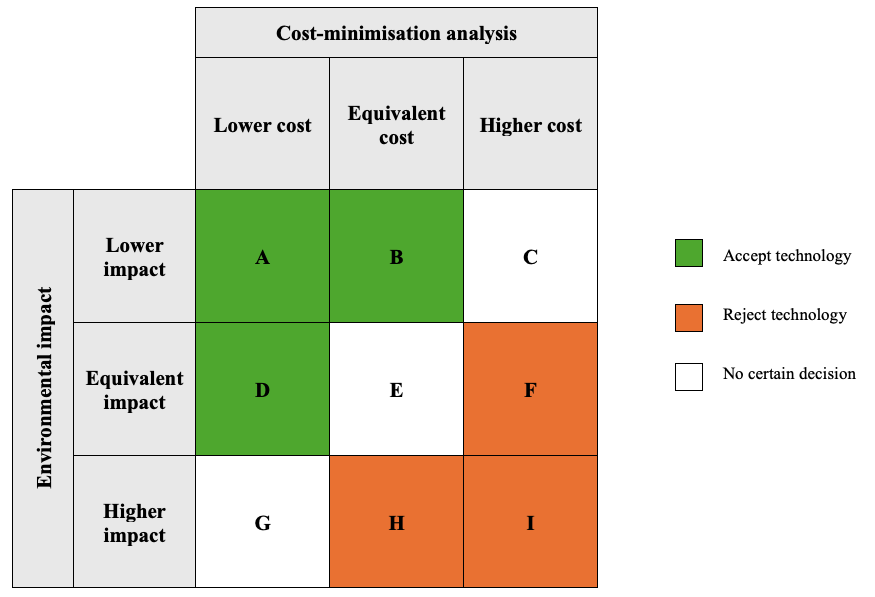
\includegraphics[width=1\linewidth]{core-chapters/figs/ch-9-fig-1.png}
    \caption{Decision making matrix for cost-minimisation analysis and environmental impacts, assuming acceptability of trade-offs between costs and carbon emissions.}
    \label{fig:ch-9-fig-1}
\end{figure}

Decisions might also be made when the proposed technology has equivalent costs and lower or higher environmental impacts. In these scenarios, environmental outcomes can be used as a decision modifier to either accept (Scenario B) or reject (Scenario H) the technology. These two decisions are environment-focused in their approach as they deal with technologies that are not expected to have health or cost benefits. 

The socially optimal decision is less certain in the remaining three scenarios. Two of these occur when the proposed technology has lower environmental impacts but higher costs (Scenario C), or higher environmental impacts but lower costs (Scenario G). There has been very little research undertaken to understand public perspectives about these types of trade-offs, and no work has been undertaken in the Australian context. The final scenario is when both the cost and environmental outcomes – as well as the health gains – are neutral (Scenario E). In this case, the HTA agency would need to look at other factors to make a recommendation. 

The benefit of the decision matrix in Figure 1 is that it makes explicit how and when environmental impacts might be considered by an HTA agency – something that is not generally clear in the parallel evaluation approach. It also does not rely on MCDA or the identification of explicit weighting of criteria and may therefore be acceptable and easier to implement in Australian where there is no precedent for using MCDA in HTA.

\section{Future research and conclusions }
If environmental impacts are to be considered routinely in Australian HTA, several outstanding challenges that need to be addressed. These include methodological issues related to integrated evaluations, such as discount rates, willingness-to-pay thresholds, and whether impacts should be considered a cost or benefit. Methods are also limited by a lack of knowledge about societal preferences concerning the trade-off between health outcomes, costs, and environmental impacts.

One potential limitation of considering the environmental impacts of health technologies through formal HTA pathways is that HTA is only undertaken for new technologies. Any move to consider environmental impacts in HTA should therefore ideally be accompanied by measures over time to also consider the environmental impact of already approved health technologies, which constitute a high proportion of spending. While HTA bodies do not currently review already approved technologies, the HTA Review recommends the Australian Government update post-review frameworks for evaluation (Recommendation 18), opening an opportunity to also consider environmental impacts in this process. 

In this article we have outlined the current Australian policy context, evaluated potential methods in the Australian context, and proposed a simple decision matrix to guide the parallel interpretation of environmental impacts alongside cost-minimisation analysis. We do not propose this method as a complete solution to the challenges of including environmental impacts in HTA. Instead, we propose it as a relatively simple and effective starting point for developing a more comprehensive methodological approach to considering environmental impacts in Australian HTAs. \textcolor{white}{\cite{national_institute_for_health_and_care_excellence_hta_nodate} \cite{noauthor_health_2025} \cite{canadian_agency_for_drugs_and_technologies_in_health_health_2015} \cite{benard_environmental_2025} \cite{canadas_drug_agency_ahead_2022}}

\printbibliography[heading=subbibliography]
\end{refsection}
\chapter{Discussion}
\label{ch-10}

\begin{refsection}[refs/ch-ten.bib]

This thesis was designed to explore how environmental impacts can be included in health technology assessment (HTA), with a focus on HTA for devices and drugs in the Australian reimbursement decision making context. It explored economic and environmental methods to estimate the environmental impact of healthcare technologies, reviewed methods to include these impacts in economic evaluations and HTA, and explored how these could form part of the Australian HTA decision making processes. This chapter outlines the principal findings of the research, summarises implications for research and policy, outlines the strengths and limitations of the body of work, and gives recommendations for future research. 

\section{Principal findings}
This thesis contains seven chapters that add new knowledge to the healthcare sustainability and health economics literature. Five of these have been published in peer-reviewed journals, and the remaining two have been submitted for publication and are currently under review. The findings of each chapter are summarised in Table 1. 

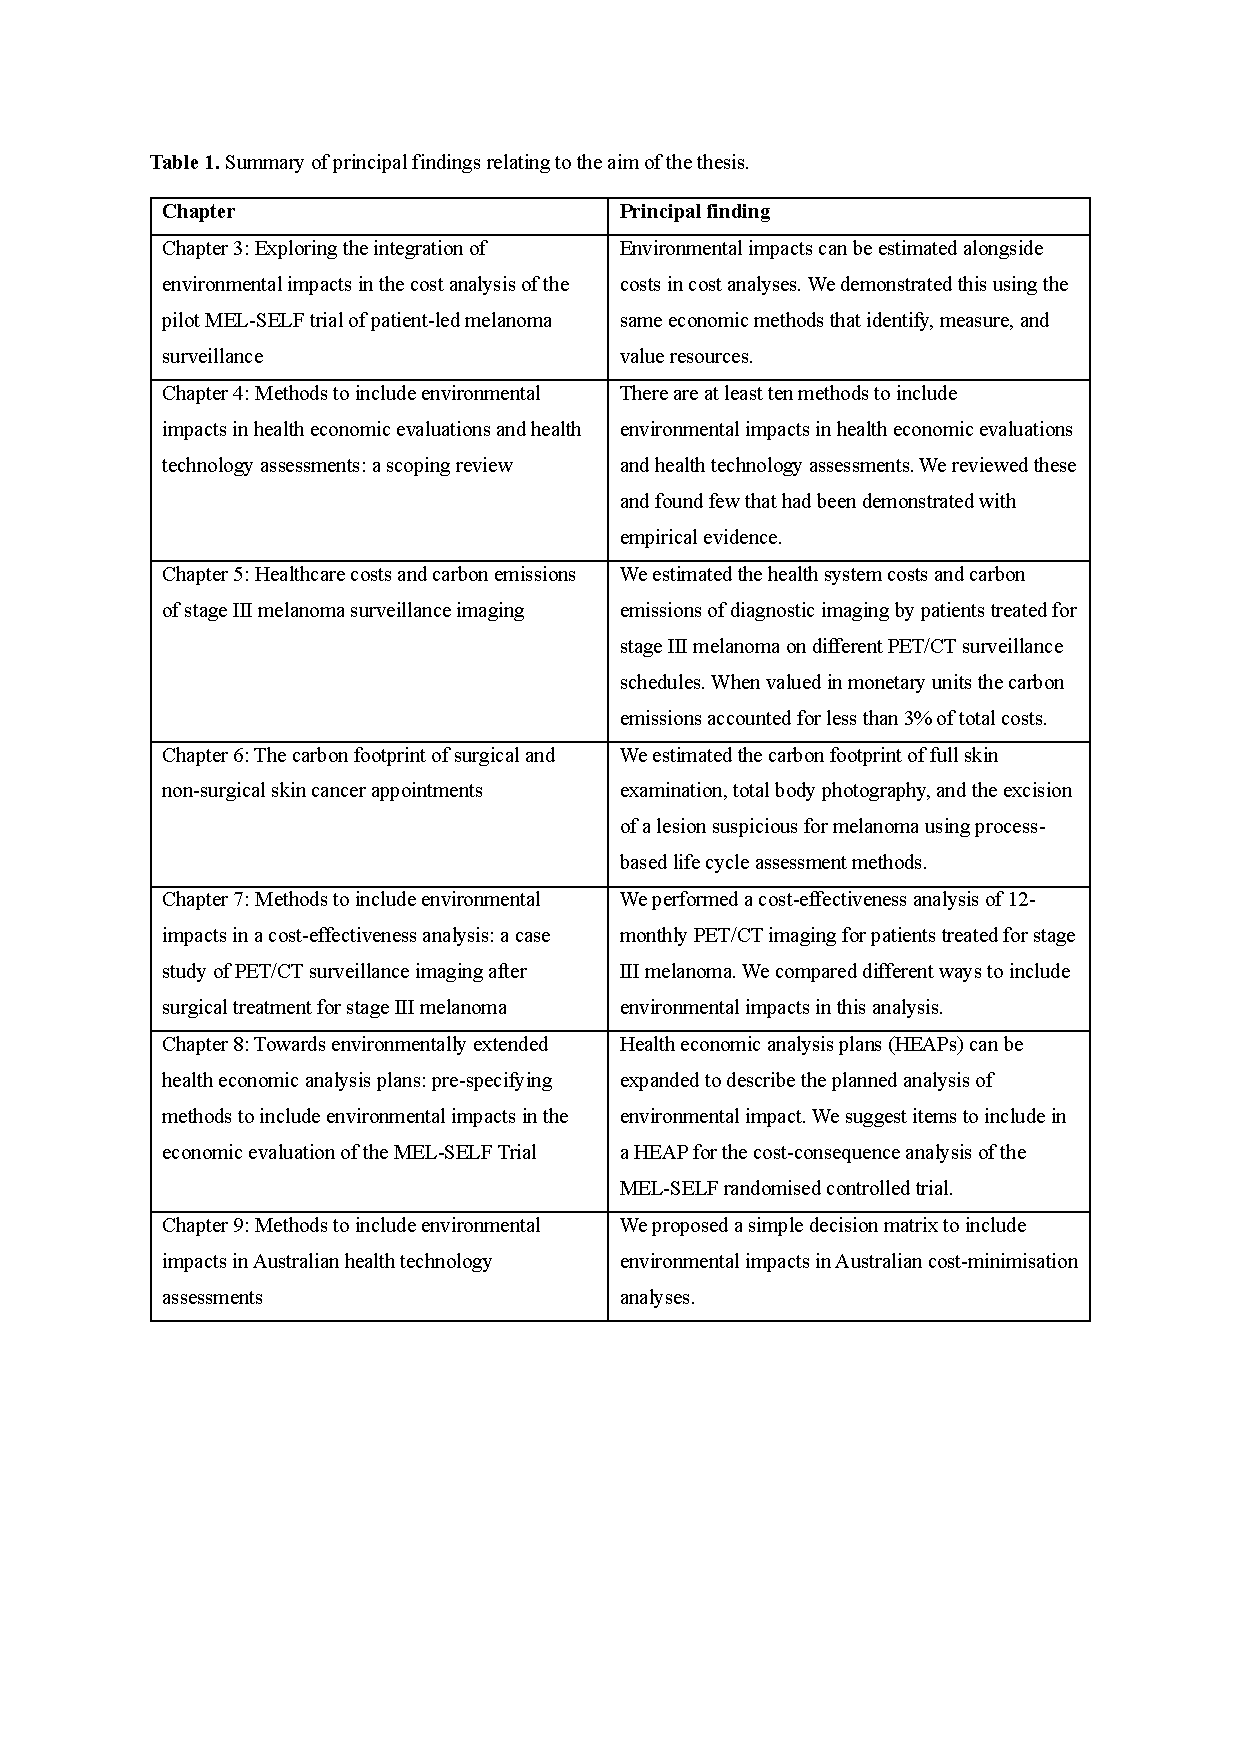
\includepdf[]{core-chapters/ch-10-tab.pdf}

Chapter 3 described an approach to include environmental impacts in a cost analysis and demonstrated this approach using the example of the MEL-SELF pilot randomised controlled trial. It was published in \textit{Applied Health Economics and Health Policy}. It found patients receiving patient-led and clinician-led surveillance, on average, cost the health system \$759 each, were associated with \$88 in productivity losses, incurred \$183 in out-of-pocket costs, and generated 10 kg CO$_{2}$-e from patient transport over the six-month study period. This study demonstrated environmental impacts, particularly carbon emissions, can be estimated alongside health costs in economic cost analyses, and doing so follows the same economic methods which identify, measure, and value healthcare resources. This study did not report any health outcomes, and it remained unclear how the environmental impacts could be included in full economic evaluations.

Chapter 4 reviewed and summarised evidence about methods to include environmental impacts in health economic evaluations and health technology assessments. It was published in \textit{Value in Health}. Two types of study were identified. The first identified, measured, and/or valued environmental impacts in a health economic context, with methods similar to those described in Chapter 3. The second demonstrated or described methods to include environmental impacts in an economic evaluation. Ten methods were grouped into four approaches: information conduit, parallel evaluation, integrated evaluation, and environment-focused evaluation. Only six studies demonstrated these methods, and none were from an Australian context. We found that while methods to include environmental impacts in HTA and economic evaluation existed, they had not been tested for use and further work was needed explore their application for real-world decision making. 

Chapter 5 estimated health system costs and carbon emissions of diagnostic imaging undertaken by patients on different PET/CT surveillance schedules for the follow up of stage III melanoma. It was published in \textit{Applied Health Economics and Health Policy}. It found patients in more frequent imaging schedules (i.e. scheduled imaging every 3-6 months) incurred higher healthcare costs and carbon emissions than patients managed with less frequent imaging schedules (i.e., scheduled imaging once per year). This study also explored the valuation of carbon emissions in monetary units and found emissions accounted for a small proportion (1.8-2.6\%) of total costs.

Chapter 6 estimated the carbon emissions of skin cancer clinic consultations. It is currently under review with \textit{Clinical and Experimental Dermatology}. The study used process-based life cycle assessment methods to estimate emissions in carbon dioxide equivalent units (CO$_{2}$-e). We explored three common reasons patients visit dermatology clinics for the diagnosis and treatment of skin cancer: full skin examination, total body photography, and the excision of a lesion. Carbon emissions were 11.11, 10.75, and 12.21 kg CO$_{2}$-e respectively. Patient transport was responsible for 10.72 kg CO$_{2}$-e.

Chapter 7 demonstrated methods to include carbon emissions in a cost-effectiveness analysis of different PET/CT surveillance imaging schedules for detecting distant metastasis after treatment for stage III melanoma. It was published in \textit{Value in Health}. The study used methods identified in Chapter 4, and inputs estimated in Chapters 5 and 6. Four methods were demonstrated: reporting emissions in parallel; the incremental carbon footprint cost ratio (ICFCR); the incremental carbon footprint effectiveness ratio (ICFER); and integrating emissions as a cost in the incremental cost-effectiveness ratio (ICER). The base case analysis (without environmental impacts) found 12-monthly PET/CT imaging was more expensive and more effective than no scheduled imaging, with an ICER of \$71,857 per false negative avoided. Carbon emissions were higher for 12-monthly imaging than no routine imaging. The ICFCR was 0.2 kg CO$_{2}$-e per additional dollar spent, and the ICFER was 17,331 kg CO$_{2}$-e per false negative avoided. When emissions were integrated as a cost the ICER increased modestly to \$74,017 per false negative avoided. In this example we found incorporating carbon emissions did not change the result of the CEA unless that valuation was relatively high, for example when the mortality accounting social cost of carbon (mSCC) was used. 

Chapter 8 described the health economic analysis plan (HEAP) for the MELanoma SELF surveillance randomised controlled trial and argued that guidelines for items to include in HEAPs should be expanded for studies including environmental impacts. It was published in \textit{Applied Health Economics and Health Policy}. 

Chapter 9 explored the application of methods to include environmental impacts in the Australian HTA decision making policy context. It is currently under review with the \textit{International Journal of Technology Assessment in Healthcare}. The article outlines the Australian policy context, evaluates potential methods, and proposes a simple decision matrix to include environmental impacts in a cost-minimisation assessment pathway.

\section{Implications}
The findings of this research have implications for health economists and for policy makers considering including environmental impacts in HTA and these are summarised in the following sections. 

\subsection{Implications for health economists and researchers}
There is a growing body of literature exploring how environmental impacts can be included in health economic evaluations and HTA, which was reviewed in Chapter 4 and by other recent studies.\cite{polisena_environmental_2018, pinho-gomes_incorporating_2022, guirado-fuentes_main_2023, desterbecq_inclusion_2023, antonazzo_health_2025} This work has largely focused on methodological descriptions and reviews, and, despite the empirical contributions of this thesis and of some other notable studies,\cite{de_preux_beyond_2018, kindred_exploratory_2024, dunbar_balancing_2025, marsh_incorporating_2016, kingma_exploring_2025} there is a lack of evidence demonstrating these methods. The cost-effectiveness analysis reported in Chapter 7 is the first Australian study of its kind and can be used by future studies seeking to include environment impacts in their analyses. There are two main implications of this research for health economists and other researchers.

First, economic methods are ideal for estimating the expected environmental impact of health technologies. In the empirical chapters of this thesis, we included carbon emissions in economic studies by identifying, measuring, and valuing resource use, such as healthcare services and patient travel. This is consistent with methods used in economic evaluations to estimate the costs and benefits of a technology.\cite{drummond_methods_2015} For example, in Chapter 5 we identified the use of diagnostic imaging tests, measured the number of times each test was used, and valued these using existing carbon emission estimates per test. Similar approaches were used in Chapters 3 and 7. This represents a modest addition to the work usually conducted in an economic evaluation to estimate the cost of the health technology, providing emissions factors for resources are already known.

Most economic evaluations do not usually derive resource unit costs de novo and instead rely on data from existing sources. The exception to this is in the case of micro-costing studies where there are no available estimates. Economic evaluations could follow the same principles for environmental impacts and rely on data from existing life cycle assessments (LCA), such as those indexed by the HealthcareLCA database or the recently announced Lancet MedZero.\cite{drew_healthcarelca_2025, watts_lancet_2025} Doing so would more efficiently use the limited healthcare-focused LCA workforce than conducting an LCA for every economic evaluation. It is also simpler for health economists to implement than requiring them to learn and conduct LCA within their studies. While there is currently a lack of high quality LCAs that can be relied on for economic evaluation inputs, LCAs only need to be conducted once per resource (for a particular time and place) and can then be relied on by future economic evaluations. 

If an LCA is conducted as part of the broader project it should be reported separately to the economic evaluation, as in the LCA reported in Chapter 6 for the cost-effectiveness analysis in Chapter 7. This ensures health economists can rely on their skills and do not need the specialist expertise or software required to conduct an LCA. It also ensures the LCA study is reviewed and published in sufficient detail and quality as to be useful to future economic evaluations. This might be less likely if the LCA is reported within an economic evaluation (i.e. with limited word count for the methods to facilitate replication).

Second, it showed including environmental impacts in economic evaluations is feasible and can be done in several ways. Once economic methods have been followed to estimate the environmental impact of the technology, it is methodologically simple to then include these in the evaluation, as described in Chapter 4 and demonstrated in Chapter 7. Different approaches and methods can be used by analysts with the most important differences being whether to integrate impacts into the evaluation (or consider them in parallel) and whether to value them in health, monetary, or environmental units. Consensus on the best approach has not been reached, especially in the context of health technology assessment, but this shouldn’t stop economic evaluations from exploring these methods further and contributing to much-needed empirical evidence of how proposed methods work in practice. Chapter 8 showed how to include environmental impacts in health economic analysis plans (HEAPs) for studies contributing to this body of work. This work might support, and be supported by, arguments for using a societal perspective, and for considering other broader costs and benefits in the economic evaluation.

In this thesis we found evaluations that include environmental impacts might reach the same conclusion about value for money as an identical evaluation that does not include environmental impacts. There are two reasons for this. First, in our case studies more costly health technologies had higher environmental impacts than less costly ones. While the cost of a technology and its carbon emissions are not directly linked, and carbon emission estimates based on monetary healthcare costs are unlikely to be valid,\cite{mcalister_how_2024} in the examples presented in Chapters 3, 5, and 7 we found that higher cost interventions also had higher emissions. Therefore, including emissions in the analysis may only reinforce the interpretation that would have been made without their inclusion. The exception to this may be when environmental impacts are integrated as a cost or benefit in a cost-effectiveness analysis. Here, considering the additional impacts may change the interpretation of value-for-money.

Second, and more importantly, the value of environmental impacts relative to the monetary cost of the technology or the health benefit appears to be small and difficult to interpret when common valuations are used. For example, in Chapter 7 of this thesis we found that when valued in Australian Dollars (AUD) and integrated into a cost-effectiveness analysis environmental impacts accounted for less than 3\% of total costs. This was true even when higher valuations (e.g. a higher social cost of carbon) were applied to the analyses and is consistent with the findings from other recent work.\cite{ducrot_integrating_2025} In Chapter 7 we identified the mortality accounting social cost of carbon (mSCC) as a potential value for carbon emissions. This is orders of magnitude higher than other social costs of carbon and did meaningfully impact the result of the cost-effectiveness analysis.

When environmental impacts are reported parallel to the economic evaluation the interpretation is difficult because we have little guidance about public and decision maker preferences for the trade-offs between health outcomes and environmental impacts. What would it mean for a technology that has an incremental cost-effectiveness ratio less than \$50,000 AUD but an increase of 100 t CO$_{2}$-e? Or, for a technology with an incremental carbon footprint effectiveness ratio of 100 t CO$_{2}$-e per quality adjusted life year gained? While these can be calculated and reported, their interpretation is difficult without understanding the preferences for the trade-offs taking place or the willingness-to-pay to reduce emissions. 

\subsection{Implications for policy makers}
As described in Chapter 1 and 9, Australian HTA does not require environmental impacts to be considered in by the applicants or the evaluators. The findings of this thesis show that health economic evaluations can be expanded to include environmental impacts, and there are plausible methods to include these in HTA for reimbursement decisions. However, further work is needed to address knowledge gaps before this can be done routinely.

Chapter 9 explores how guidelines for submissions to the Australian Medical Services Advisory Committee (MSAC) currently allow environmental impacts to be submitted as part of an application for reimbursement, and the HTA Review has proposed to explore how this can be done as part of an assessment of the technology’s cost-effectiveness. The primary challenge for the implementation of any of the feasible methods identified in this thesis is that we do not currently understand societal preferences for trade-offs between healthcare costs, health outcomes, and environmental impacts. Are we willing to spend more from the health budget to reduce carbon emissions and climate change? Would society trade potential health gains for individuals now, for carbon emissions reductions that benefit people in the future? What are society’s preferences for policy change related to the above to mitigate climate impacts? In Chapter 9 we proposed a simple decision matrix for Australia’s cost-minimisation pathway that partially avoids this issue by only considering environmental impacts when health outcomes are equivalent. While this may be useful in some scenarios, it is not known how often it would be useful. If HTA are to routinely consider environmental impacts, then this should be done systematically and not only in cost-minimisation analyses. 

There are also some practical implications for policy makers. First, guidelines for applications to MSAC, PBAC, and other similar bodies will need to be updated and made consistent to facilitate or require environmental impacts to be submitted with applications. This should contain specifics useful to the applicants, including what environmental impacts should be submitted, how they should be included, and how they will be considered. The answer to all these questions will depend on the context. It may also require additional expertise to be added to the advisory committees that review HTA applications and an upskilling of the epidemiological and health economic workforce to understand and report these data. Guidance will also need to be given about how this information will be interpreted once received by the committee. Considerations will need to be given as to how this might impact the speed of assessments and, at least initially, this is unlikely to be a compulsory requirement of HTA.

It remains unclear how often environmental impacts would influence HTA decisions. In their seminal textbook on methods for the economic evaluation of health care programmes, Drummond et al. suggest that the main “contribution of economic evaluation may not be in changing the decisions that are ultimately made but how they are made”.\cite{drummond_methods_2015} The findings of this thesis suggest that including environmental impacts may not change decisions that would have been made based on standard methods that do not include environmental impacts. However, as with the suggestion by Drummond et al. this does not mean it is not worthwhile. Rather, by including environmental impacts we can provide “proper accountability for the social choices made on behalf of others”.\cite{drummond_methods_2015} In the context of climate change this accountability is a worthwhile justification for including environmental impacts in economic evaluations. 

\section{Strengths and limitations}
The strengths of this thesis include its various methodological approaches, relying on costing, cost-effectiveness, and life cycle assessment methods to explore approaches to include environmental impacts in health technology assessment. It uses these alongside Australian case studies and policy perspectives to fill an important gap in the literature.

However, there are also limitations of this thesis. Limitations of each chapter are discussed in detail in the respective Discussion section of the chapter. Overall, this field has rapidly evolved since the first of the empirical chapters were designed and published. Because of this, methods and literature were less explored in those studies than in later Chapters. An example of this is the note in Chapter 4 that no study had explored the inclusion of environmental impacts on the benefits side of an economic evaluation as a QALY. However, by Chapter 7 a study was referenced demonstrating exactly that. Furthermore, we have not demonstrated all identified methods empirically and there remains a sizeable gap of evidence in this area. Future work should be coordinated and avoid further duplication of these research outputs.\cite{hensher_climate_2023}

\section{Future research directions}
Based on the findings of this thesis we make the following recommendations for future research directions.

First, we note in several chapters that the interpretation of environmental data is hindered by a lack of evidence about the preferences and attitudes of the public and of decision makers. HTA decisions are made on the behalf of society and reflect their preferences. Methods that include environmental impacts in HTA should be implemented based on an understanding of the preferences for these methods. Qualitative studies are needed to explore the methods discussed in this thesis, as well as public preferences for the potential underlying trade-offs between healthcare budgets, health outcomes, and environmental impact. Some pilot work has been conducted by NICE in the UK and future work is needed to explore these perspectives in contexts that consider including environmental impacts in their HTA processes, such as Australia.\cite{nice_nice_2023}

Second, there are outstanding economic methodological questions that need to be explored. While this thesis has focused on overall methods to include environmental impacts in HTA there are outstanding questions that need to be addressed for these methods to be routinely used. This includes questions about the time horizon of analyses, and how methods accounting for future damages are considered in evaluations of technologies with shorter time horizons; the discounting of environmental impacts and whether discounting future environmental impacts is appropriate or not; and the perspective from which the analysis is conducted (e.g., health system or societal). The health economic analysis plan presented in Chapter 8 suggests these be reported, but further work is needed to explore them empirically.

Finally, as prefaced in Chapter 8, we will include environmental impacts in the economic evaluation of the MEL-SELF randomised controlled trial. This will be informed directly by the findings of this thesis. Work is also needed to explore methods to include environmental impacts in economic evaluations conducted alongside randomised controlled trials that use other economic study designs, such as within-trial cost-utility analysis and Markov modelling. 

\section{Conclusion}
This thesis aimed to explore methods to include environmental impacts in health technology assessments. It described and evaluated several of these in the Australian healthcare reimbursement decision making context. It found economic evaluation frameworks are a useful way to estimate, present, and compare the environmental impact of health technologies. Further work is needed to understand how these can most usefully be implemented to inform HTA decisions in Australia and globally. 

\printbibliography[heading=subbibliography]
\end{refsection}


\appendix % Appendix
\chapter{Correction: Exploring the integration of environmental impacts in the cost analysis of the pilot MEL-SELF trial of patient-Led melanoma surveillance}
\label{ap-a}

% PDF of published paper
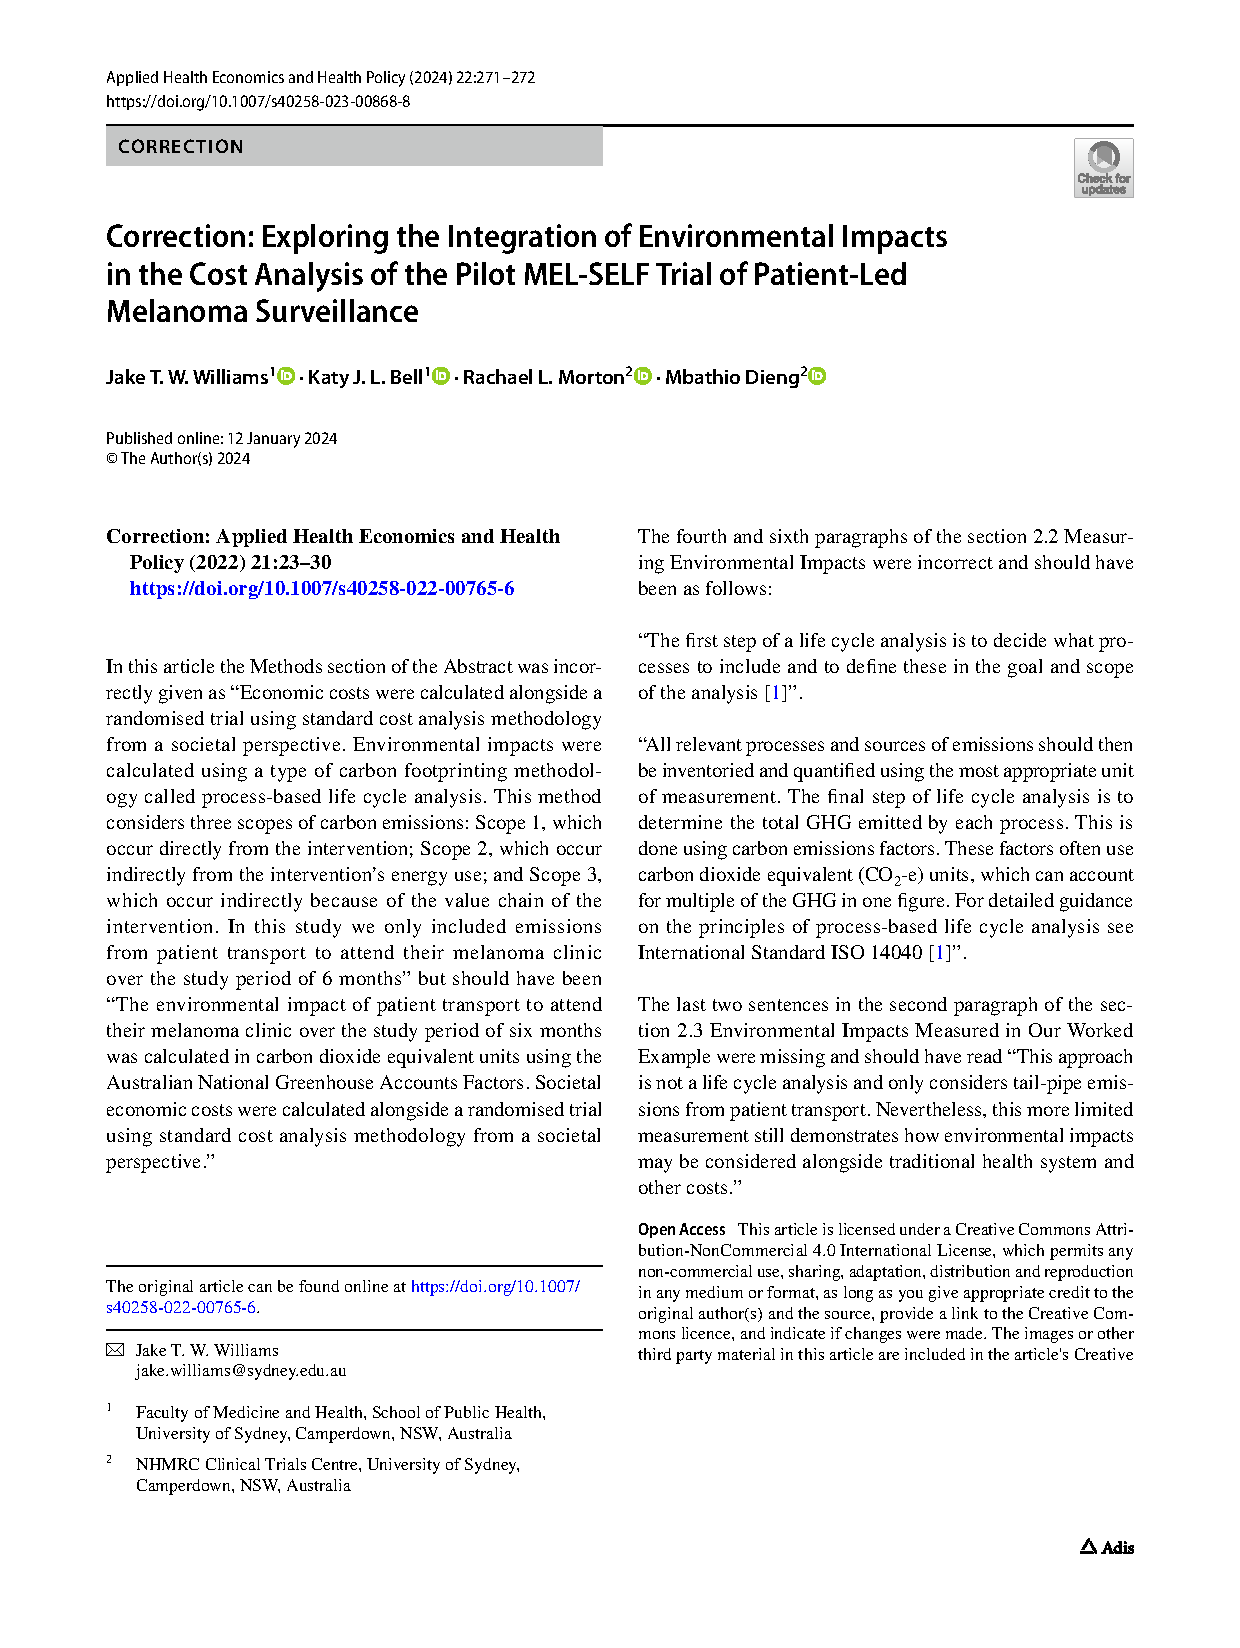
\includepdf[pages=-]{pdfs/ap-a.pdf}
\chapter{Supplementary information for Chapter 4}
\label{ap-b}

% PDF of published paper
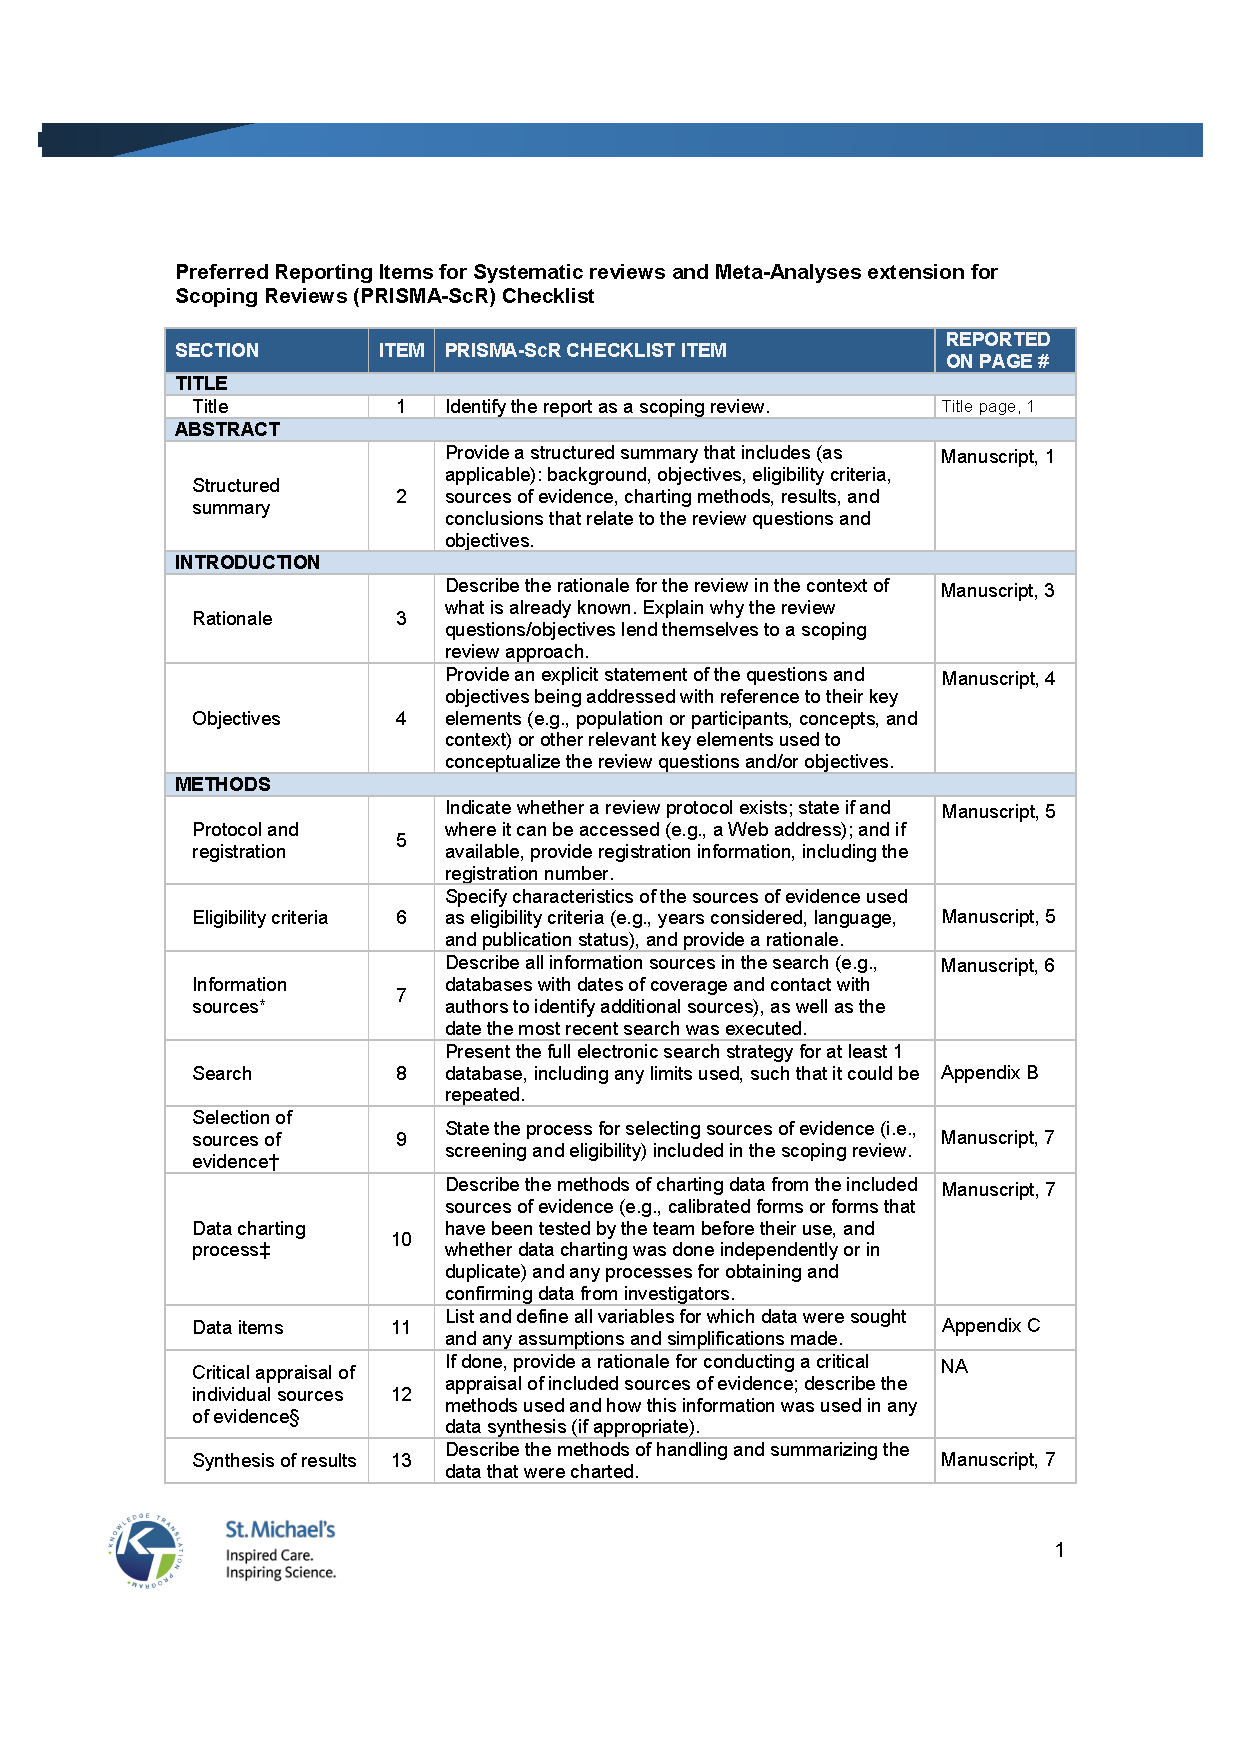
\includepdf[pages=-]{pdfs/ap-b-1.pdf}
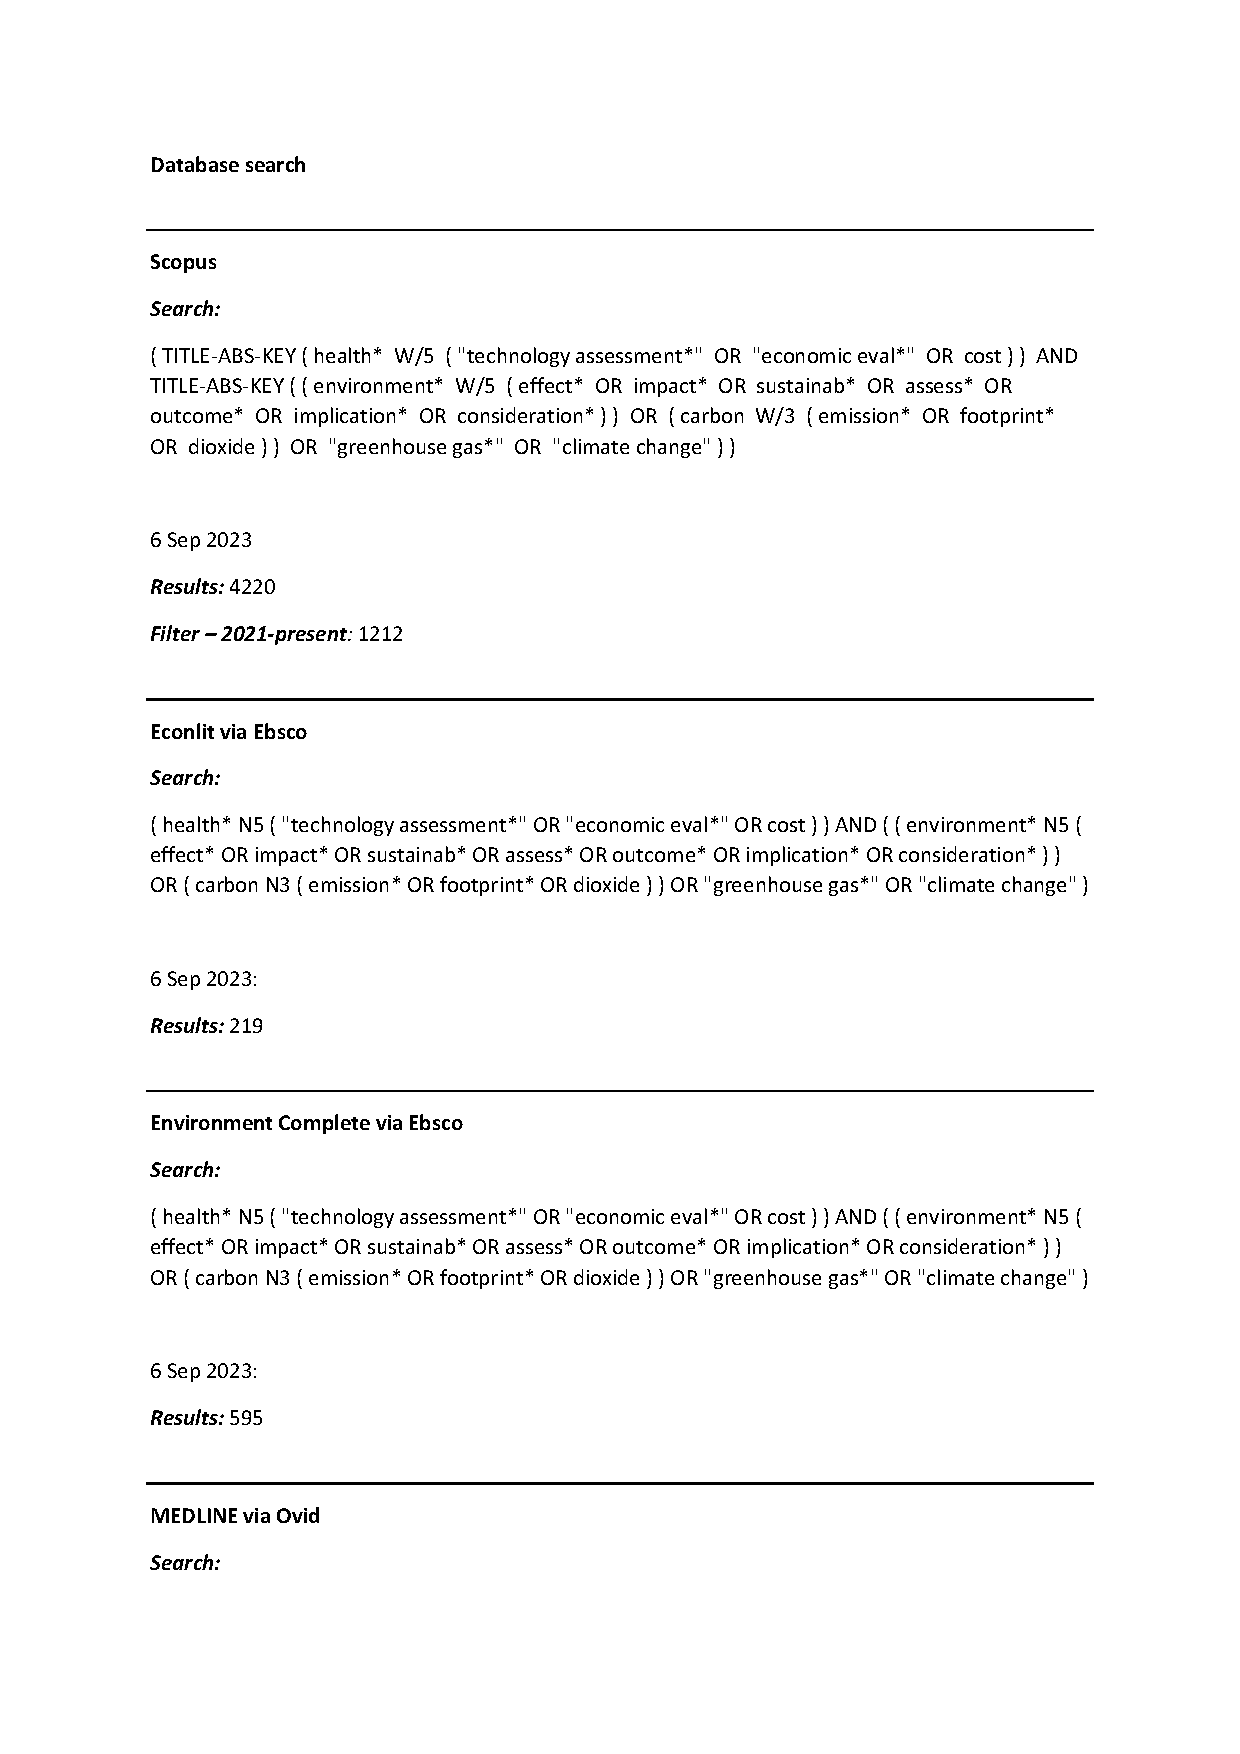
\includepdf[pages=-]{pdfs/ap-b-2.pdf}
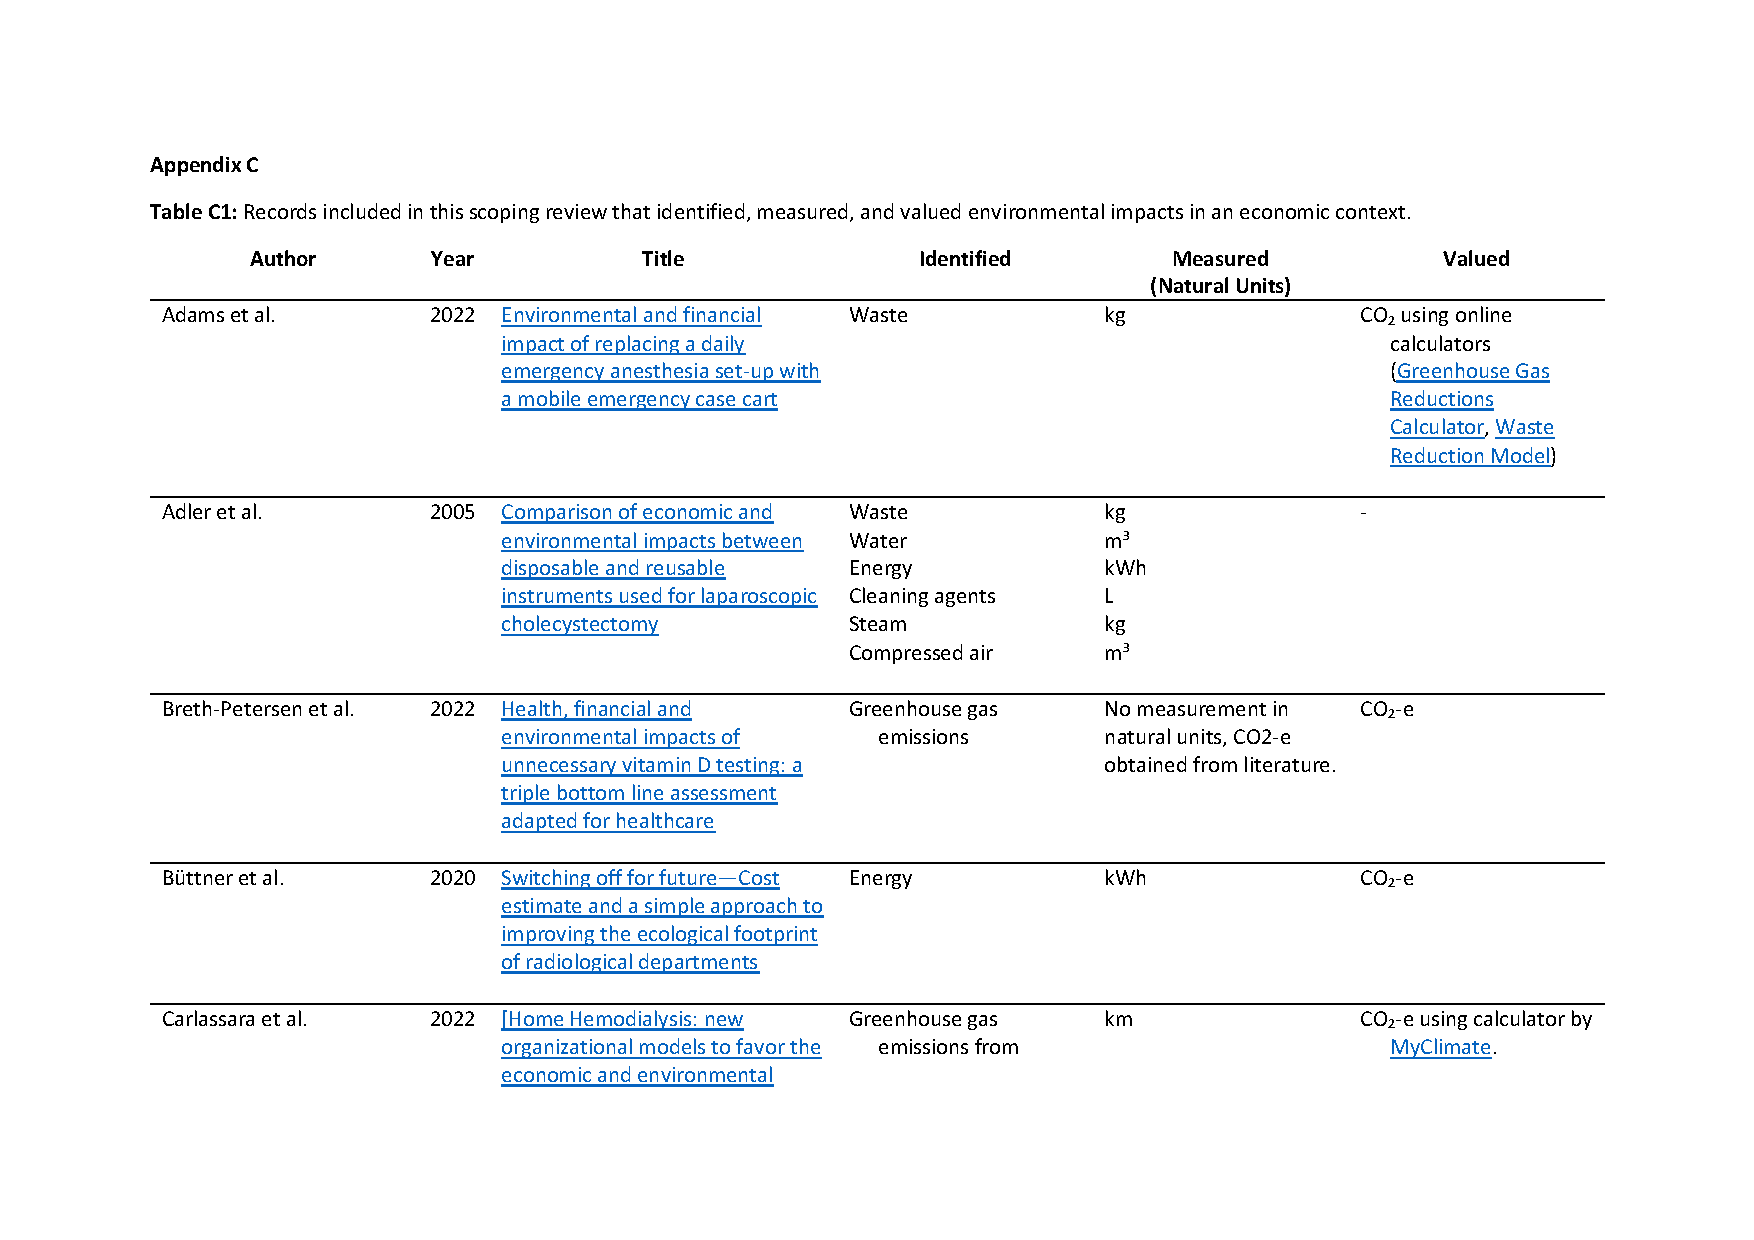
\includepdf[pages=-, angle=90]{pdfs/ap-b-3.pdf}
\chapter{Protocol: Methods for including environmental impacts in health economic evaluations and health technology assessments: a scoping review}
\label{ap-c}

% PDF of published paper

\includepdf[pages=-]{pdfs/ap-c.pdf}
\chapter{Supplementary information for Chapter 5}
\label{ap-d}

% PDF of published paper
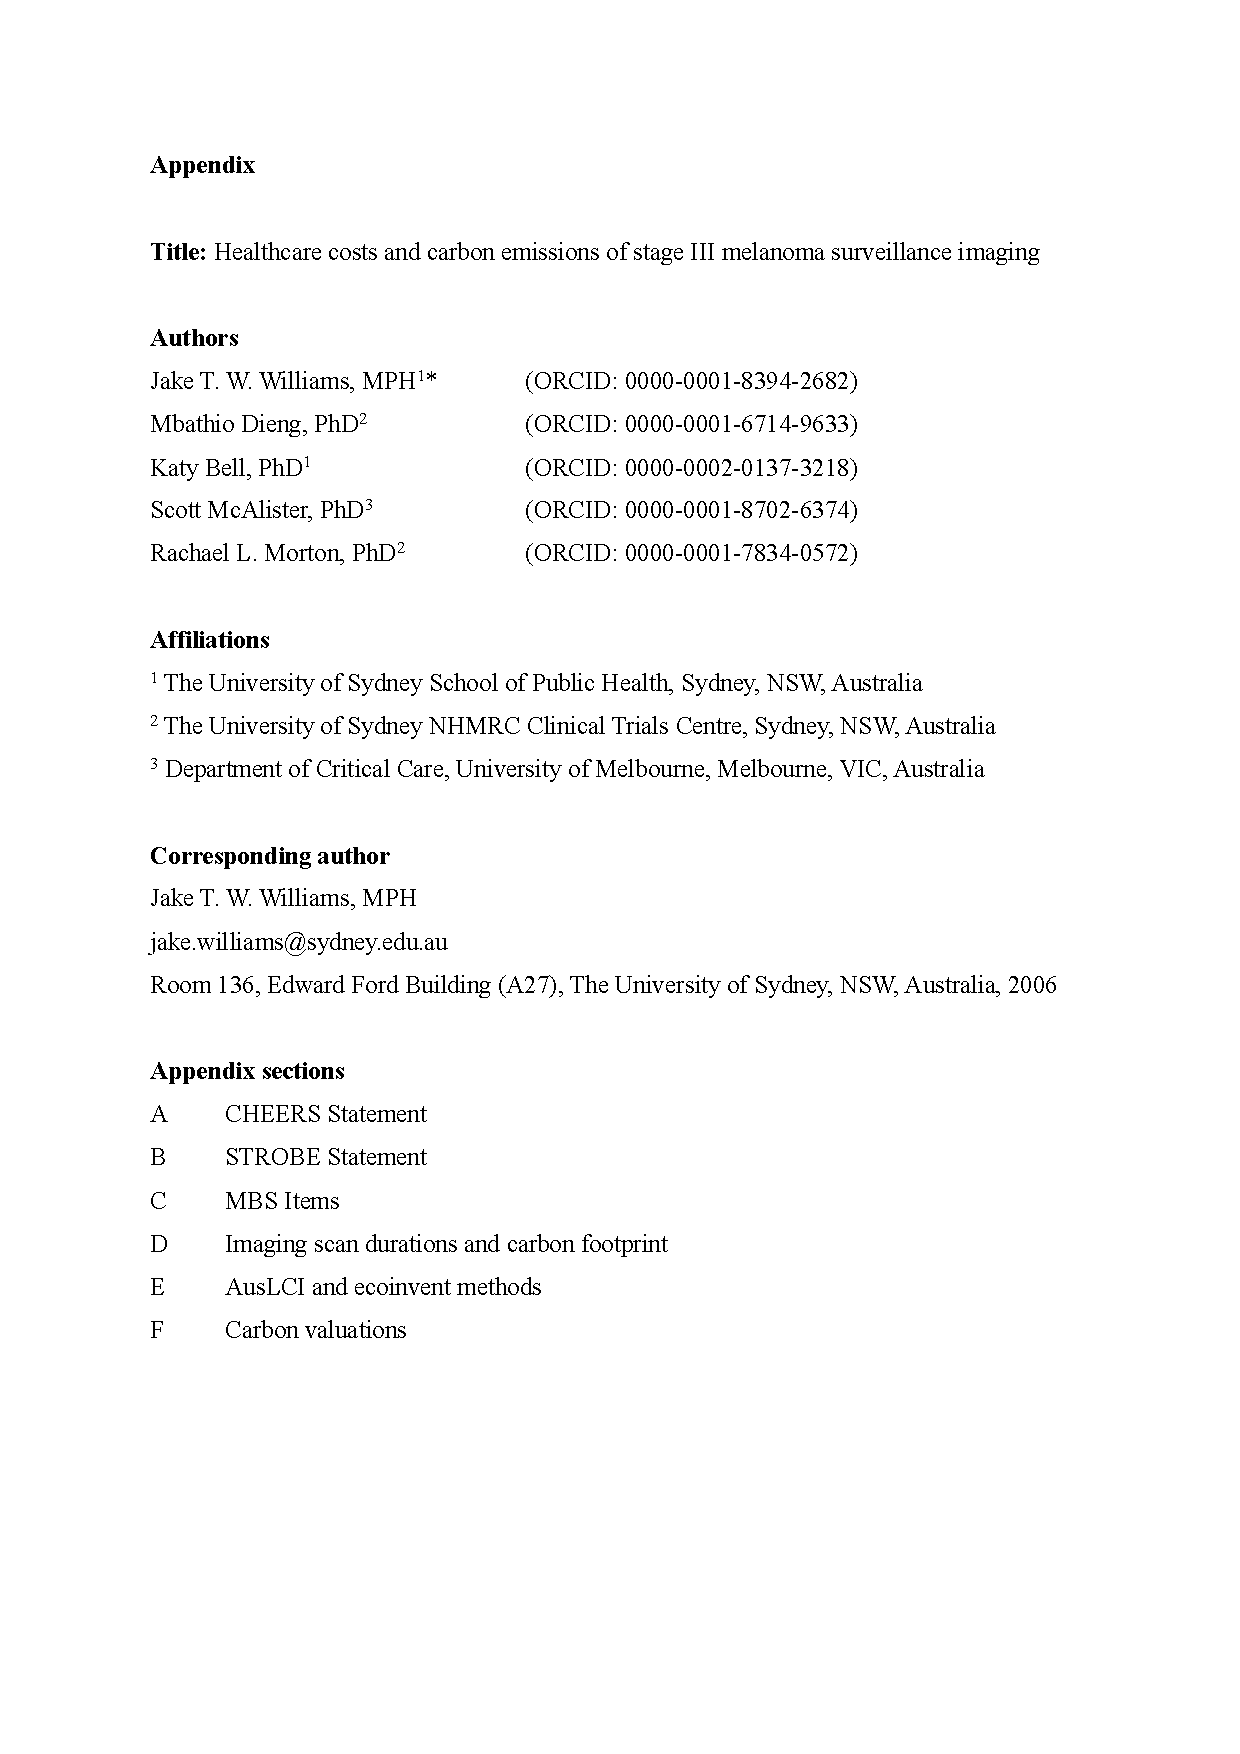
\includepdf[pages=-]{pdfs/ap-d.pdf}
\chapter{Supplementary information for Chapter 6}
\label{ap-e}

% PDF of published paper
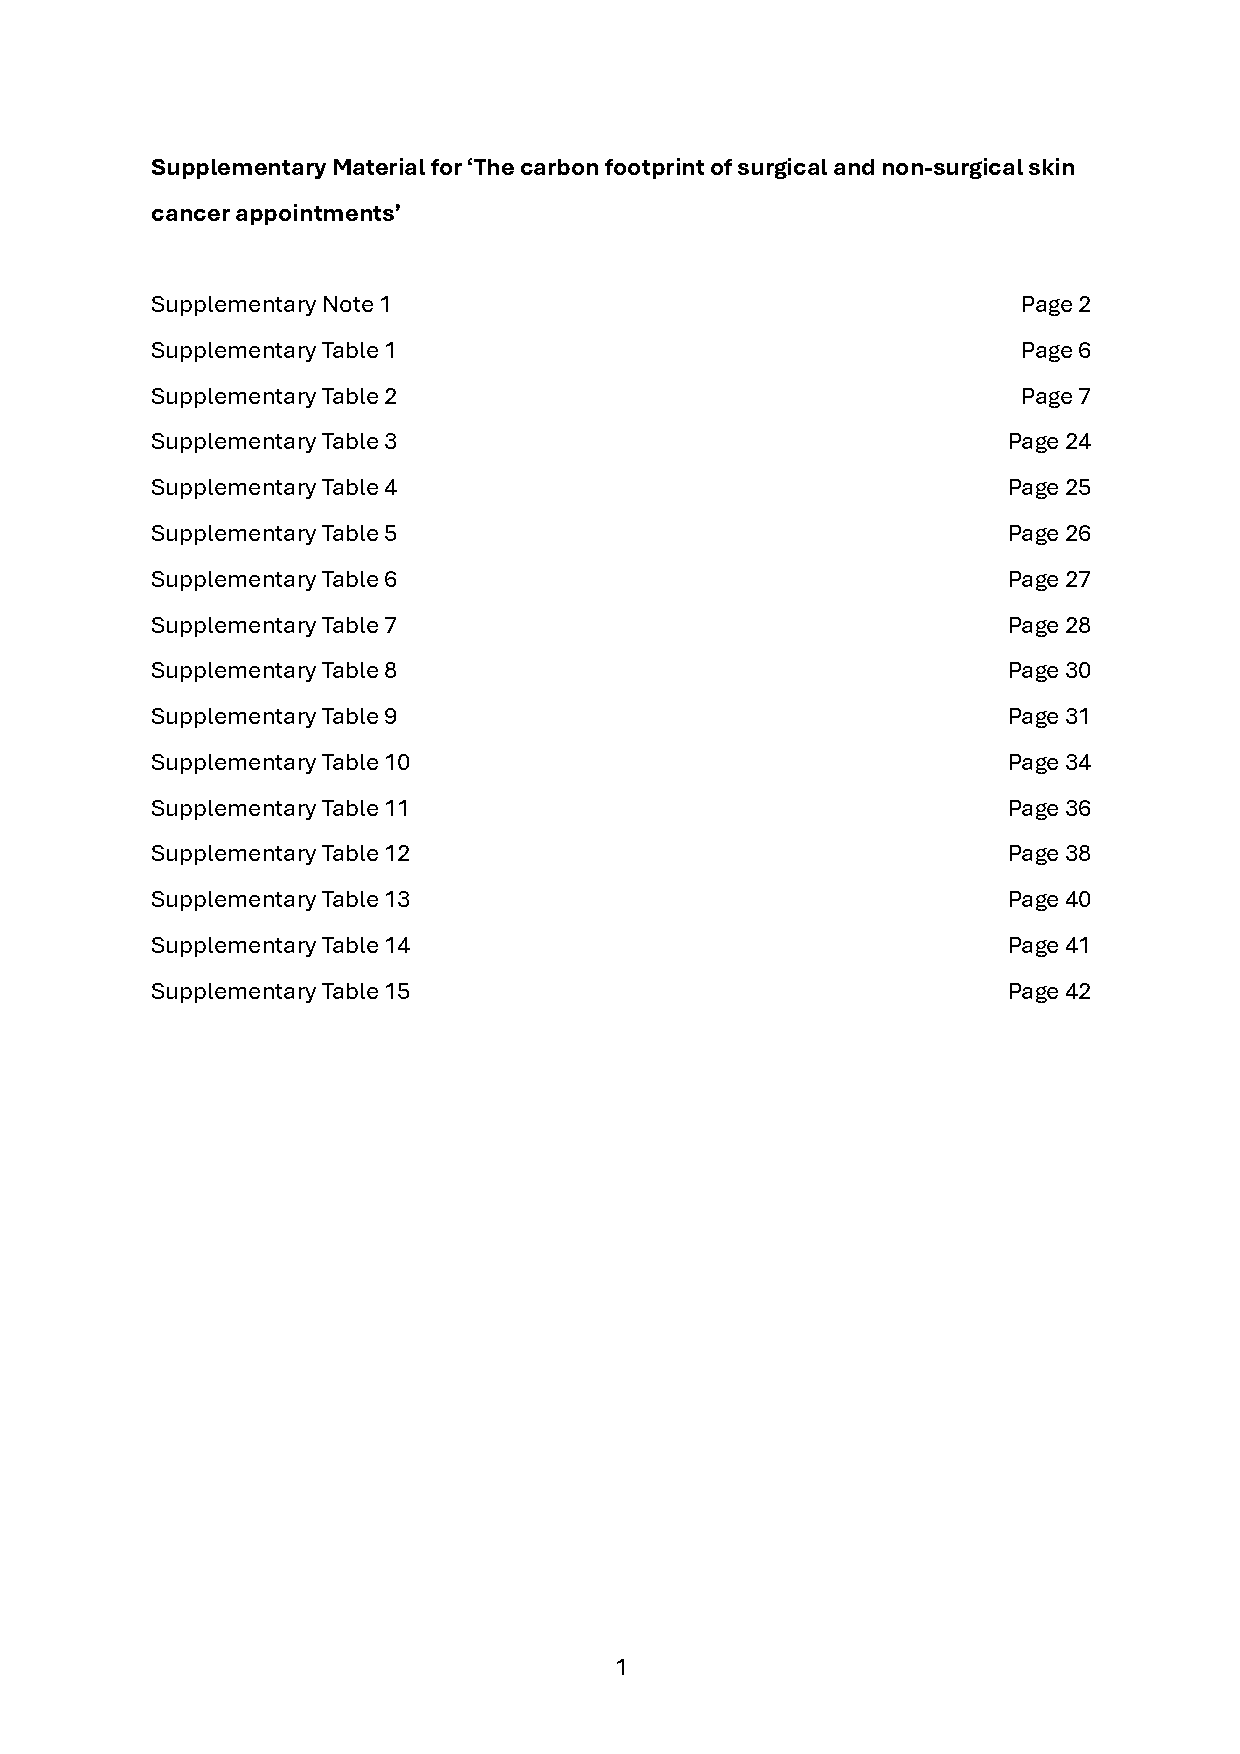
\includepdf[pages=-]{pdfs/ap-e.pdf}
\chapter{Protocol: The Climate Change Impact Of Surgical And Non-Surgical Skin Cancer Appointments: A Process-Based Life Cycle Assessment}
\label{ap-f}

% PDF of published paper

\includepdf[pages=-]{pdfs/ap-f.pdf}
\chapter{Supplementary information for Chapter 7}
\label{ap-g}

\clearpage

% PDF of published paper
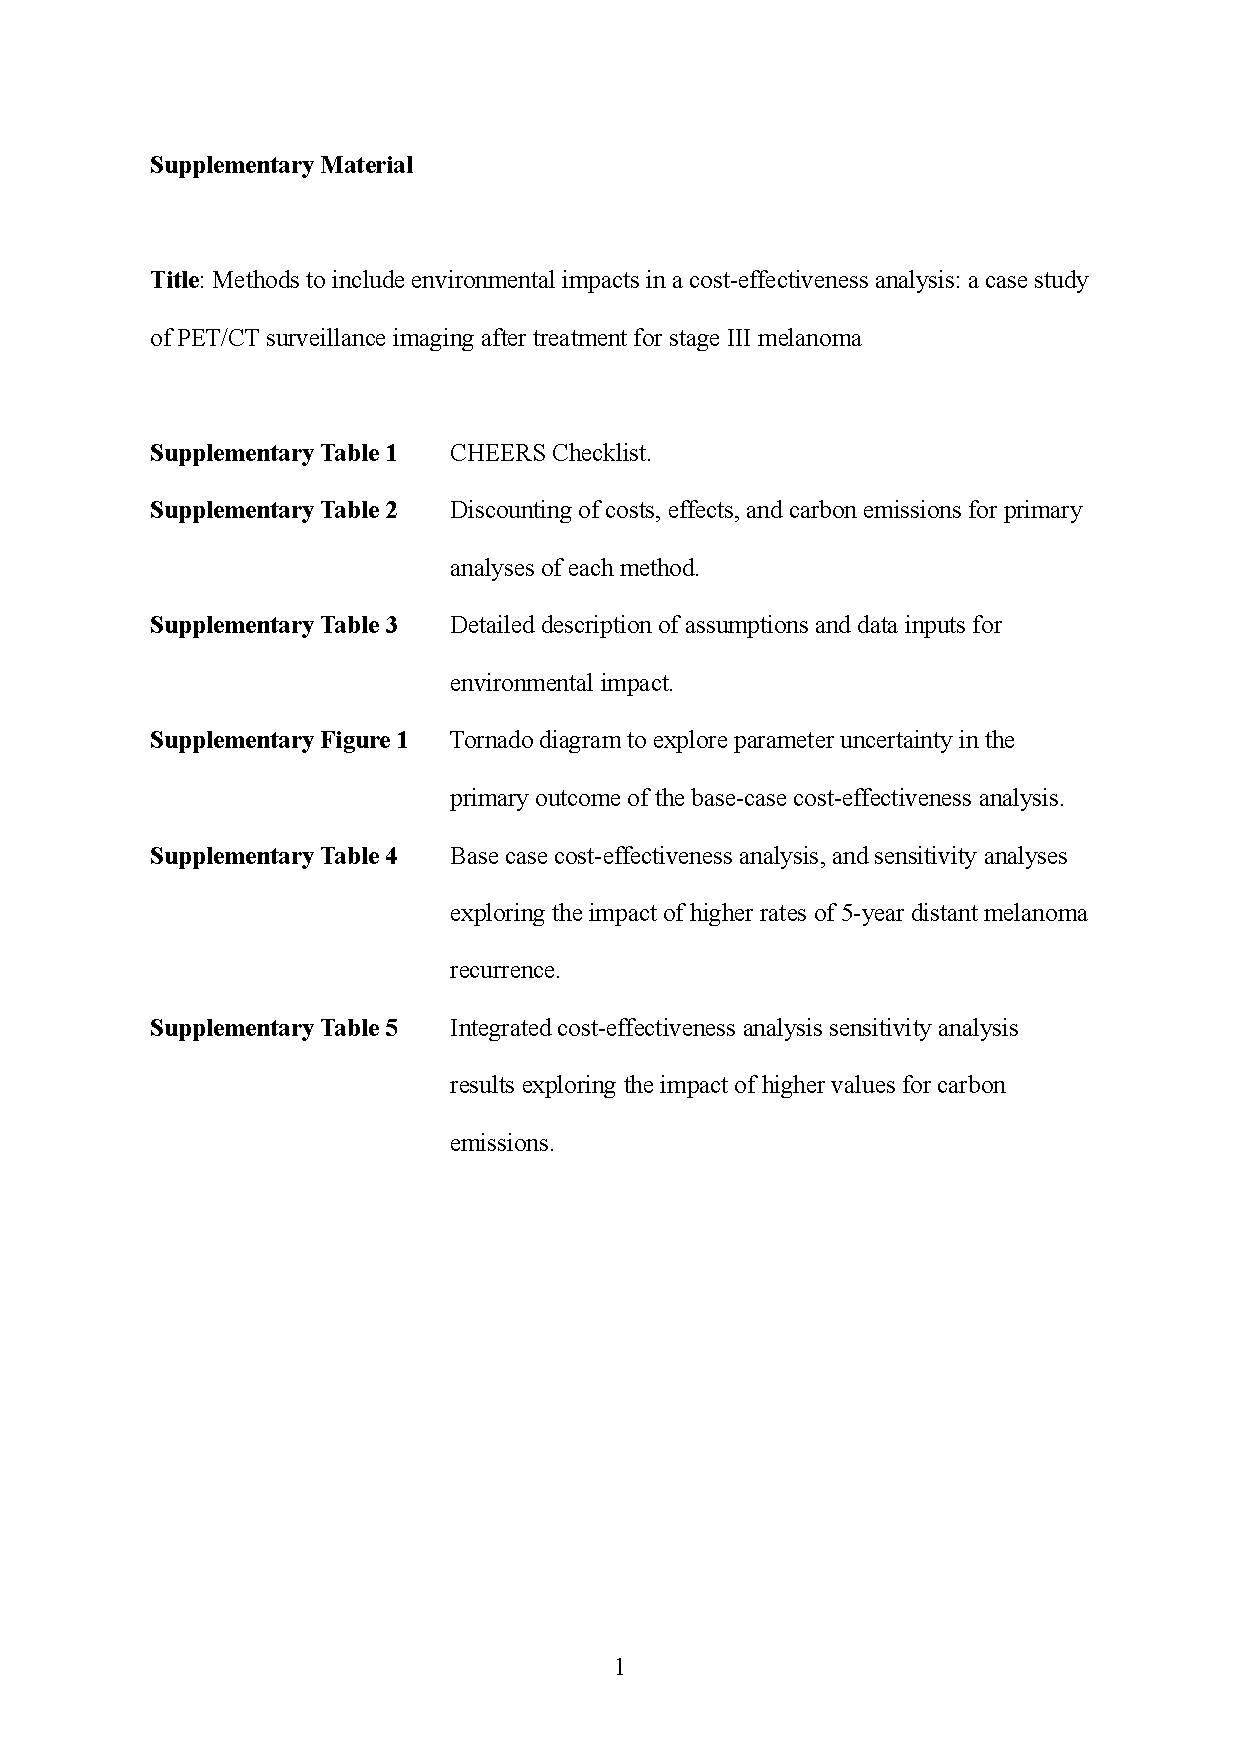
\includepdf[pages=-]{pdfs/ap-g.pdf}
\chapter{Health economic analysis plan for the MELanoma SELF surveillance (MEL-SELF) trial}
\label{ap-h}

% PDF of published paper
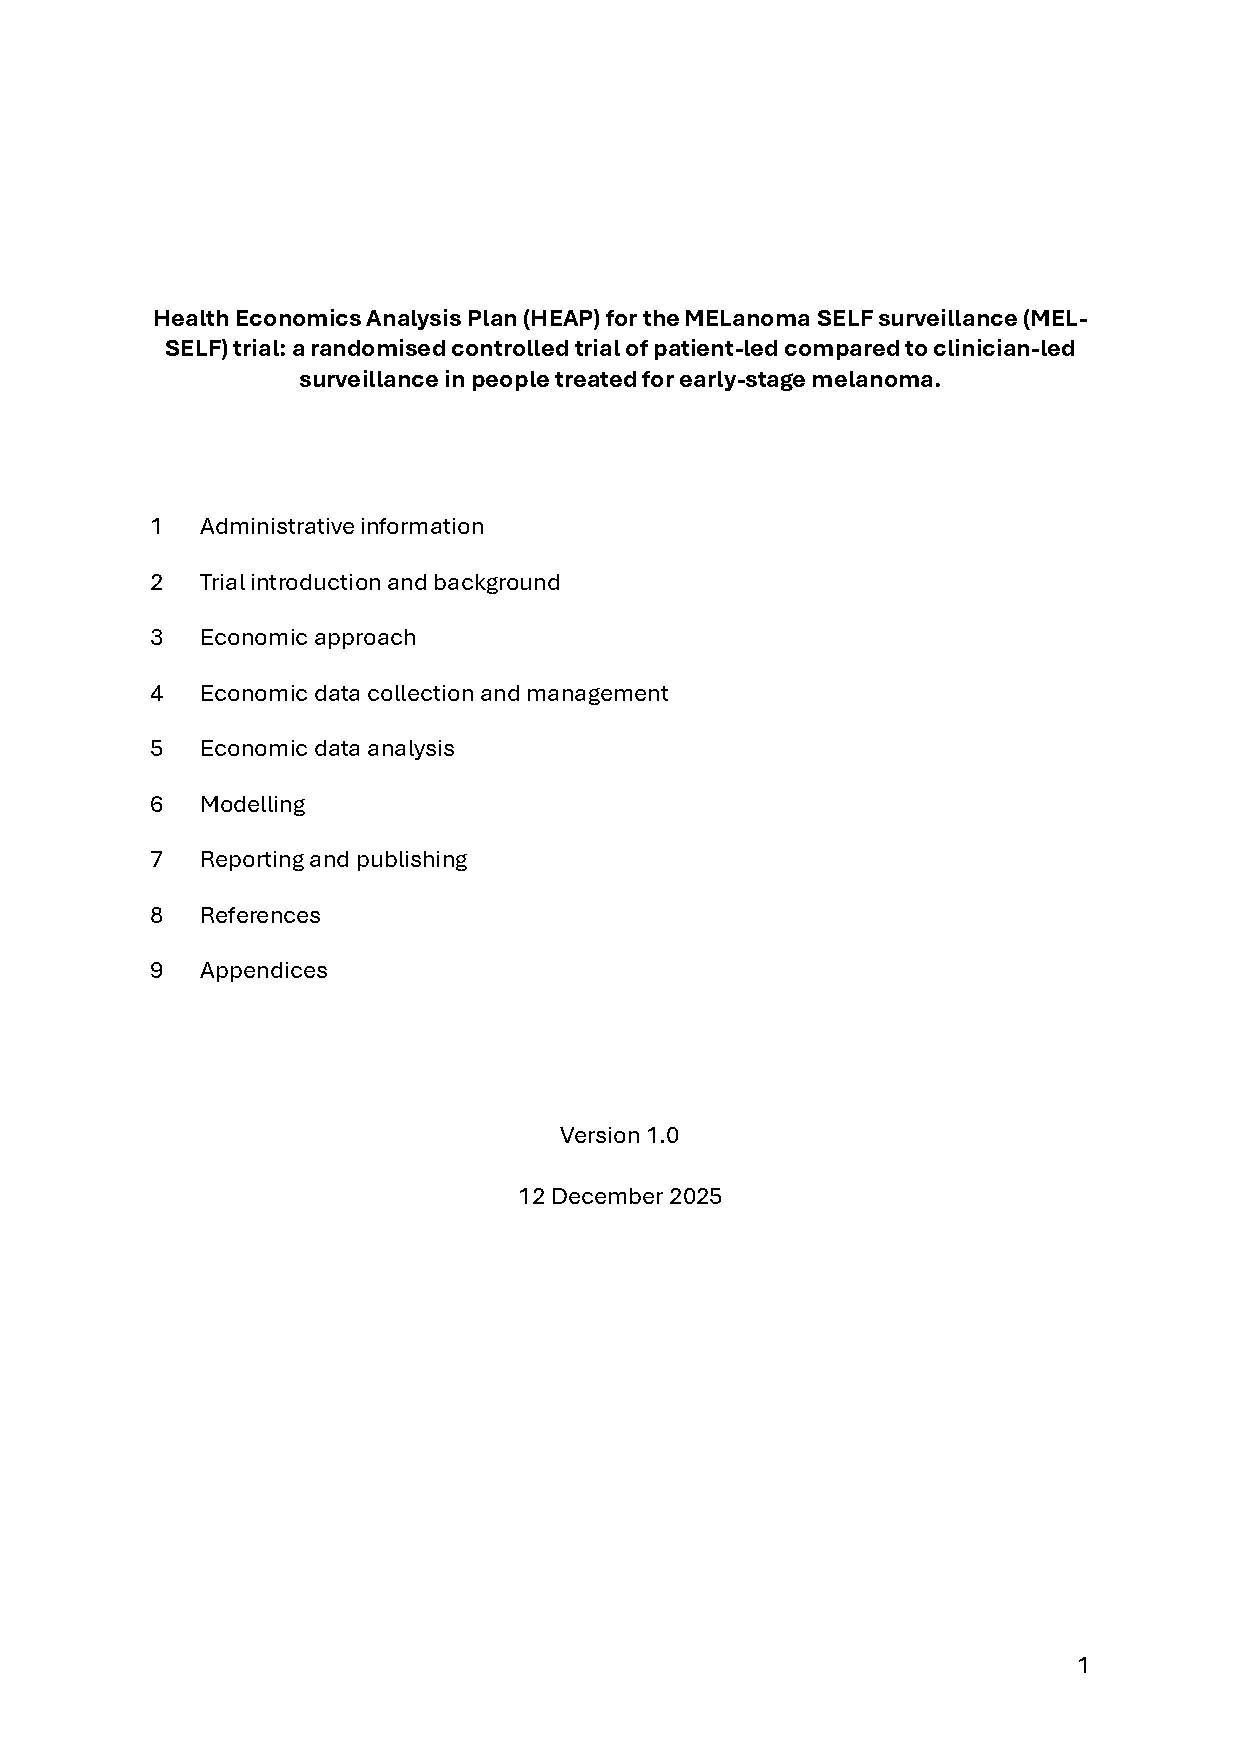
\includepdf[pages=1-3]{pdfs/ap-h.pdf}
\includepdf[pages=4, angle=90]{pdfs/ap-h.pdf}
\includepdf[pages=5-44]{pdfs/ap-h.pdf}
\chapter{Deeble Institute issues brief 58: consideration of environmental impacts in health technology assessment}
\label{ap-i}

\paragraph*{Publication details}
\textit{Williams J} and Haddock R. Consideration of environmental impacts in health technology assessment. Australian Healthcare and Hospitals Association Limited, Australia. 2025 Jun 5, Deeble issues brief 58.

% PDF of published paper

\includepdf[pages=-]{pdfs/ap-i.pdf}

\clearpage

\end{document}

